\documentclass{grattan}
% Comments are deployed by the % sign; everything after % is ignored by the compiler.
% Please do not put comments before \documentclass as these are reserved for TeX directives.
%!TEX root=../Report.tex

\usepackage{bbding}
\usepackage{environ}
\makeatletter
\newsavebox{\measure@tikzpicture}
\NewEnviron{scaletikzpicturetowidth}[1]{%
  \def\tikz@width{#1}%
  \def\tikzscale{1}\begin{lrbox}{\measure@tikzpicture}%
  \BODY
  \end{lrbox}%
  \pgfmathparse{#1/\wd\measure@tikzpicture}%
  \edef\tikzscale{\pgfmathresult}%
  \BODY
}
\makeatother

\usepackage{pgfplots}
% Aspect ratio by inspection
\pgfplotsset{width=\columnwidth, height=0.66\columnwidth, compat=1.9}



% Appendix
\usepackage{longtable}
\usepackage{nameref}
%\usepackage{microtype}

\LTchunksize=100
\providecommand{\xtablewidth}{\linewidth}

\AtBeginEnvironment{quote}{\small\justifying}

% For the main matter
% Floates
\crefname{reco}{Recommendation}{Recommendations}
\Crefname{reco}{Recommendation}{Recommendations}
\DeclareFloatingEnvironment[listname={List of recommendations}, name = {Recommendation}]{reco}

\counterwithout{reco}{chapter}

\newenvironment{recobox}[2][htbp]{%
\setlength{\currentparskip}{\parskip}%
\begin{reco}[#1]
\begin{mdframed}[style=GrattanFrameBox]
\setlength{\parskip}{\currentparskip}
\captionsetup{labelfont={bf,Orange},font={bf,Orange},format=plain,justification=raggedright,singlelinecheck=false, skip=0ex, position=above}
\caption{#2}
\raggedright
}{
\end{mdframed}\end{reco}%
}

\providecommand{\kmh}{km\,/\,h}

% \newcommand{\microtypeforquote}{\microtypecontext{spacing=nonfrench}
% % http://tex.stackexchange.com/questions/303457/setprotrusion-with-helvetica-on-specific-characters
% \SetProtrusion
%    [ name     = T1-phv,      % the name is optional
%      load     = T1-default ] % first load `T1-default` settings
%    { encoding = T1,
%      family   = phv }        % use for Helvetica family
%    {
%      \textendash = {-25, }, 
%      \textemdash = {-25, },  % cancel out left protrusion
%      \textquotedblleft = {1000,}
%    }
% }
\providecommand{\microtypeforquote}{}


\usepackage{zref-user}
\makeatletter
\zref@newprop{chapter}{\thechapter}
\@ifundefined{@chapapp}{\let\@chapapp\chaptername}{}
\zref@newprop{chaptertype}{\@chapapp}% as suggested by Danie Els
\zref@addprop{main}{chapter}
% \zref@addprop{main}{chapter,chaptertype}
\makeatother

\hyphenpenalty=700
\YEAR{2017}

% add_to_dictionary: freeway freeways Anzac Hoddle Bertauld Marchetti Zahavi automobile densification arterials?
% add_to_dictionary: Epworth Yarra DWLs? spacing=nonfrench measurability Measurability polycentric
% add_to_dictionary: Drummoyne Balmain Balgowlah Mosman Cremorne Freeway Westlink WestConnex
% add_to_dictionary: flagfall NorthConnex IPART untolled Artarmon Warringah expressway Arncliffe
% add_to_dictionary: Dandenong La Trobe Kew Donnybrook Frankston Sunbury Craigieburn Camberwell
% add_to_dictionary: Rowville CityLink EastLink Freeways Oakleigh Cranbourne Coburg Moonee Ponds
% add_to_dictionary: Clem Glenroy rollover Greensborough Footscray Bundoora SEK Keilor Watsonia
% add_to_dictionary: Macleod Nunawading Spotswood Altona Essendon Somerton Truganina Mernda Morang
% add_to_dictionary: Parkville Seaford Carrum Prahran Southbank Braybrook Chadstone Bentleigh
% add_to_dictionary: CBD Keilor East Macquarie Park Sydney Tennyson Smithfield Green Valley Bossley Park Newport Collaroy Plateau Dee Why Mona Vale
% add_to_dictionary: Avalon Beach Cronulla Willoughby East Zetland Vaucluse Randwick Paddington Mosman Maroubra Roseville Leichhardt Riverview Killara Wareemba Drummoyne Bellevue Hill Cremorne Coogee Bondi Beach Bronte Balgowlah Jannali Menai Gymea Bay Engadine Caringbah South St Clair Cambridge Park Chifley Kensington Blacktown Springwood Kingswood South Penrith Glenmore Park Emu Plains Cranebrook Blaxland Old Toongabbie North Parramatta Merrylands Greystanes Camden Eschol Park Ryde Epping Eastwood Cherrybrook Carlingford Prestons West Hoxton Holsworthy Chipping Norton Casula Wentworth Falls Hazelbrook Ambarvale Mount Annan Minto Macquarie Fields Thornleigh Berowra Heights Mount Colah Warriewood Allambie Heights Manly Beacon Hill Panania Kellyville Stanhope Gardens Middle Dural Baulkham Hills Ruse Narellan Bradbury Seven Hills Quakers Hill Lalor Park Oakhurst Woodcroft Marayong Glenwood Yagoona Greenacre Georges Hall Prospect Neutral Bay Padstow Fairfield West Port Melbourne Box Hill North Glen Iris Watsonia Vermont South Preston Ashfield Ipswich Herston North Lakes Woolloongabba Banyo New Farm Brisbane West Footscray Forestville Tempe Parramatta Burwood Pennant Hills Parkville Mernda Berwick Cranbourne North Seaford Bankstown Airport Penrith Pymble University of Lane Cove Palm Beach Rockdale Hammondville Westmead Balmain Liverpool Chester Hill Chatswood Bankstown North Shore Hospital University of Sydney University of NSW Norwest Business Park North Sydney Flemington West Melbourne West Pennant Hills (F3 Mt Colah) Port Botany Campbelltown Sydney Airport West Melbourne Port Brisbane Airport Altona Acacia Ridge Somerton Maribrynong Braybrook
% add_to_dictionary: South Yarra Mornington Chadstone Albert Park Richmond Clayton Docklands Yarraville Melbourne Uni Collingwood Box Hill Fitzroy Deer Park Montrose Primary School Moonee Ponds Caulfield racecourse Clifton Hill Southbank Melbourne Airport Martin Place Station Hawthorn Point Cook Bundoora Footscray Doncaster Brighton Camberwell Hoppers Crossing Oakleigh South Caroline Springs Coburg Sunshine West Cranbourne Dandenong Rowville Heidelberg Glen Waverley Essendon Northern Hospital Epping Gosford Hornsby Castle Hill Windsor Hurstville Marrickville Artarmon Bacchus Marsh Truganina Carlton Prahran St Kilda baths Essendon DFO Monash Medical Centre Lilydale High School St Albans Blackburn station Williamstown St Kilda Kew Blackburn Frankston Keilor Bentleigh North Fitzroy Sunshine Clyde Enfield Moorebank Yennora Chullora East Kew Auburn Denistone Dulwich Hill Frenchs Forest Cabramatta Moore Park Olympic Park Stadium Barangaroo Surry Hills Glebe Homebush Mount Druitt Carrum Downs Dandenong North South Morang Coburg Library Stanmore Brookvale Upper Mount Gravatt Surfers Paradise Capalaba Brisbane Entertainment Centre Rocklea Dakabin Logan Central St Lucia Indooroopilly Redfern Craigieburn Diamond Creek Sunbury Macleod Mount Waverley Nunawading Spotswood Kingsford Milperra St Marys Condell Park Freshwater Ingleburn Katoomba Miranda Oakville Eastern Creek Naremburn Sutherland Sylvania Wetherill Park Hunters Hill Donnybrook Sydenham
% add_to_dictionary: UNSW Illawarra Geelong repurposing

% add_to_dictionary: Lupton Tversky Kahnemann
% add_to_dictionary: reco Nlllrr Wolli Melbournian Melbournians RMS eTAG
% add_to_dictionary: Thompsons Sneydes Skybus Smartbus distortionary Uber Lyft manoeuver PTV VicRoads tollways? nortonpotato
% add_to_dictionary: queue duckers USyd Melburnians?
% add_to_dictionary: Mohring-Harwitz Paulo tradies hp

% stop_if_present: Westconnex Northconnex Melbournian
% stop_if_present: (?:low[^-]hanging)

% stop_if_present: [0-9][apk]m km/hr?

\addbibresource{bib/Grattan-Master-Bibliography.bib}
\addbibresource{bib/Transport.bib}

\author{Marion Terrill}
% editorial_author_only: Paul Austin
\title{Stuck in traffic? Road congestion in Sydney and Melbourne}

\hypersetup{pdfauthor={Marion Terrill and Hugh Batrouney and Sally Etherington and Hugh Parsonage and Paul Austin and Jonathan Beh},
            pdftitle={Stuck in traffic? Road congestion in Sydney and Melbourne},
            pdfkeywords={transport,road,congestion,traffic,Australia,Sydney,Melbourne,Grattan,Institute,think-tank,public policy},
            pdfproducer={LaTeX with hyperref},
            pdfcreator={pdflatex, or other tool}}

\GrattanReportNumber{2017-10}

\acknowledgements{%
This report was written by Marion Terrill, Hugh Batrouney, Sally Etherington, and Hugh Parsonage.
Paul Austin and Jonathan Beh made valuable contributions to the report.

We are very grateful to Google for making available the data underpinning the analysis in this report.
We would also like to thank government officials and industry stakeholders for valuable input to this report.

The opinions in this report are those of the authors and do not necessarily represent the views of Grattan Institute's founding members, affiliates, individual board members, reference group members or reviewers.
Any remaining errors or omissions are the responsibility of the authors.

Grattan Institute is an independent think-tank focused on Australian public policy.
Our work is independent, practical and rigorous.
We aim to improve policy outcomes by engaging with both decision-makers and the community.

For further information on the Institute's programs, or to join our mailing list, please go to: \textcolor{blue}{\url{http://www.grattan.edu.au/}}.

% OK for release

{\footnotesize
This report may be cited as:
Terrill, M., Batrouney, H., Etherington, S., and Parsonage, H\@. (2017). \emph{\mytitle}. Grattan Institute.

ISBN: 978-0-9876121-7-5

All material published or otherwise created by Grattan Institute is licensed under a Creative Commons Attribution-NonCommercial-ShareAlike 3.0 Unported License\par
}
}




\begin{document}


\begin{overview}

Australians love their cars but hate congestion. Most commuters in Sydney and Melbourne drive to work, and one of the big conversation topics in our major cities is how clogged the roads have become. Both cities are becoming more crowded: Melbourne grew by an astonishing 25 per cent over the past decade.

Both cities have adapted remarkably well to the population boom. For most people who commute by car, the trip in the morning or afternoon peak takes less than 5 minutes longer than the same trip in the middle of the night. This is because most people work in a suburb close to home.

But delays vary dramatically in different parts of each city -- and are most acutely felt by those heading into the CBD and surrounding suburbs. Sydney CBD commuters from Hurstville in the south and Balgowlah in the north face some of the worst delays: drivers spend an extra 15 minutes on the road as a matter of routine, far longer than drivers commuting over similar distances from other parts of Sydney.

Drivers into Melbourne's CBD have a worse time if they live in suburbs in the north east including Heidelberg, Kew and Doncaster. Drivers who have to use the Eastern Freeway and Hoddle Street in the morning peak are often delayed for more than 20 minutes -- much longer than drivers from other parts of the city -- and the length of the delay can vary greatly from day to day.

The findings are based on an examination of Google Maps trip-time estimates for a more than 350 routes, taken 25 times per day, collected over six months of this year. The data includes about 3.5 million observations, and offers a fresh perspective on congestion in Sydney and Melbourne.

Both cities could face traffic gridlock in future unless decisive action is taken now.

New city freeways are not the answer. There is a place for new roads, especially in new suburbs and in areas with major redevelopments, but close to the city centres it is often more effective and always cheaper to invest in smaller-scale engineering and technology improvements such as traffic-light coordination, smarter intersection design, variable speed limits and better road surfaces and gradients. We should be sceptical of the idea that big new roads are ‘congestion busters’: they cost a fortune, take years to build, and can often fill up with new traffic of their own.

More sophisticated solutions are now required. The NSW and Victorian governments should introduce congestion charging. People who want to drive on congested roads in the peak should pay a small charge to do so. The revenue should be returned to the community as discounts on car registration, and improvements to public transport. 

And as more toll roads are introduced, state governments should ensure they have the flexibility to adjust future tolls to manage traffic flows.

In the near term, Melbourne’s CBD parking levy should be doubled, to match Sydney’s and to further discourage city commuters from driving to work.

Public transport fares in both cities should be cut during off-peak periods, to encourage people to shift their travel to times when the trains, trams and buses are not overcrowded.

These reforms would deliver city-wide benefits, easing how long we spend stuck in traffic. 

\end{overview}

\begin{recommendations}

% \begin{Center}
\section*{Recommendations to act on in the next 12 months}

% \end{Center}
\subsubsection{1. More expensive parking in Melbourne’s inner city}
The Victorian Government should increase the Melbourne CBD parking space levy from about \$1,400 to about \$2,400 to match Sydney.
\subsubsection{2. Cheaper off-peak fares on public transport}
State governments should increase differences in public transport fares by time-of-day to spread demand.
\begin{itemize}
\item The Victorian Government should establish an independent price regulator to advise on fare rates and structures, along the lines of the NSW Independent Pricing and Regulatory Tribunal; and
\item The NSW Government should introduce further discounts to off-peak rail travel, and investigate lower fares during off-peak periods.
\end{itemize}

\subsubsection{3. More frequent and detailed public information about road delays}
State governments should measure and publish delays for individual roads and routes, to enable better-informed public debate about thresholds for action.
\null\vfill\null
\columnbreak
% \begin{Center}
\section*{Recommendations for better investment}
% \end{Center}
\subsubsection{4. Compare new expenditure on roads with non-construction alternatives}
Before construction of new physical road capacity, governments should publish economic analysis of the impacts of the project in comparison with non-construction options to achieve the same objective.


\section*{Recommendations for smarter pricing}


\subsubsection{5. Establish network-wide time-of-day congestion charging}
The Victorian and NSW governments should introduce time-of-day congestion pricing in the most congested central areas of each capital city, charging a low rate at peak periods in return for a freer-flowing road.
The cost to drivers should be offset by a discount on vehicle registration, with revenue from the congestion charge earmarked to spending on public transport improvements.
\subsubsection{6. Investigate independent regulation of future toll prices}
The Victorian and NSW governments should investigate and report publicly on the independent regulation of road tolls in liaison with relevant regulators.


\section*{Popular ideas we don’t recommend}

\begin{itemize}
\item A large-scale road-building program to ``beat congestion''.
\item Staggered school starting times.
\end{itemize}

\end{recommendations}





\contentspage
\listoffigures


\chapter{Have we reached a tipping point?}\label{chap:has-congestion-reached-tipping-point}

Concern about road congestion is nothing new in Australia.
In the 1890s, newspapers reported on intense frustration with horse-and-cart congestion around Sydney's waterfront.
In the 1920s, people complained about automobile congestion on the thoroughfares of Melbourne's central business district.%
    \footcite[][165]{Davison-2016-City-Dreamers}

Concern about congestion grows when the pace of change is fast.
And Australia's major cities are growing fast: over the past decade, Sydney's population has grown by around 20 per cent and Melbourne's by more than 25 per cent.%
\footcite{ABS-2016-Regional-Population-Growth}
Not only is growth fast, it's getting faster: Sydney grew by 1.86 per cent in 2015-16, up from 1.76 per cent in the previous five years, and Melbourne by 2.74 per cent, up from 2.54 per cent.\footcite{ABS-population-March-2017} Urban population growth is expected to remain strong in coming years as people continue to gravitate to the bright lights, here in Australia as around the world.

Managing more congested roads is one of the most potent challenges of rapid population growth.
Almost any road user will tell you that city roads have become busier and slower in recent years.
And they're right
(\Vref{fig:speed-Vic-freeways-vs-year}).

\begin{figure}
\caption{The average travel speed on inner-region freeways in Melbourne has declined over time\label{fig:speed-Vic-freeways-vs-year}}
\units{\kmh}
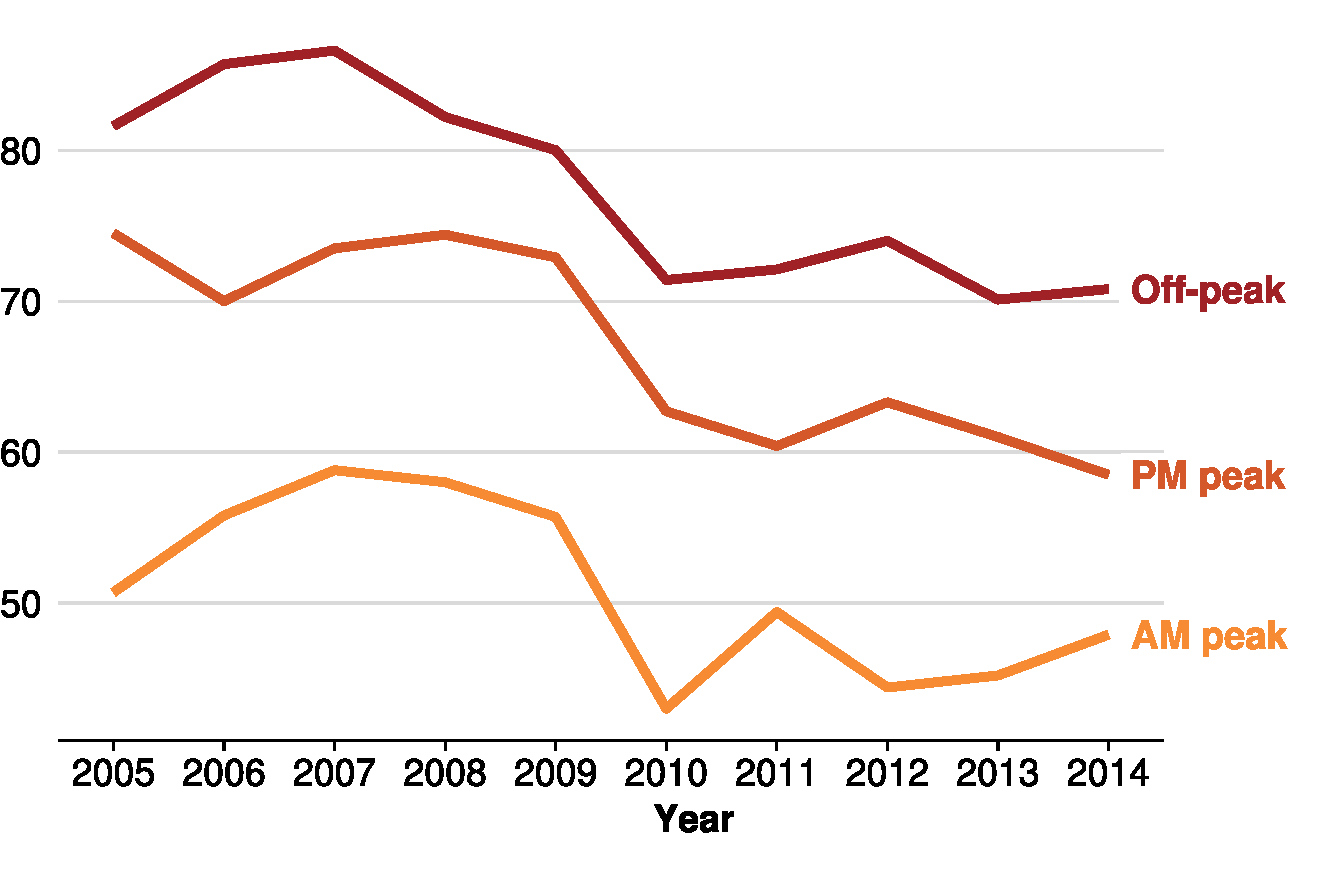
\includegraphics{atlas/freeway_speed-vs-year--MEL-1.pdf}
\noteswithsource{AM peak: 7\,am to 9\,am weekdays.
PM peak: 4:30\,pm to 6:30\,pm weekdays.
Inner-region freeways are broadly within 10-15\,km of the CBD, as detailed in \textcite[][6]{2014-VicRoads}}%
{\textcite{Vicroads-201415-TravelSpeed-tableau}}
\end{figure}

\section{Australian cities are car dependent}
City dwellers care so much about road congestion because, even in the largest cities, Australia remains a car-dependent nation. The legacy of sprawling geography and high per-capita income is one of the highest rates of vehicle ownership in the world.%
    \footcite[][9]{Austroads-2016-Congestion-Reliability-Review}

Even in Sydney, which has the highest share of public transport of any Australian city,%
    \footnote{In the 2011 Census, 25 per cent of journeys to work were on public transport in Sydney, compared with 18 per cent in Melbourne, 16 per cent in Brisbane, 14 per cent in Perth, 10 per cent in Adelaide, and 8 per cent in Canberra: \textcites{ABS2011Census}[][3]{2014-BITRE-Urban-public-transport:-updated-trends}.}
car travel overwhelmingly dominates (\Cref{fig:Mode-of-travel}).

\begin{figure}
\caption{Most people take the car to work \label{fig:Mode-of-travel}}
\units{Main mode of transport to work, by suburb of residence, Sydney}
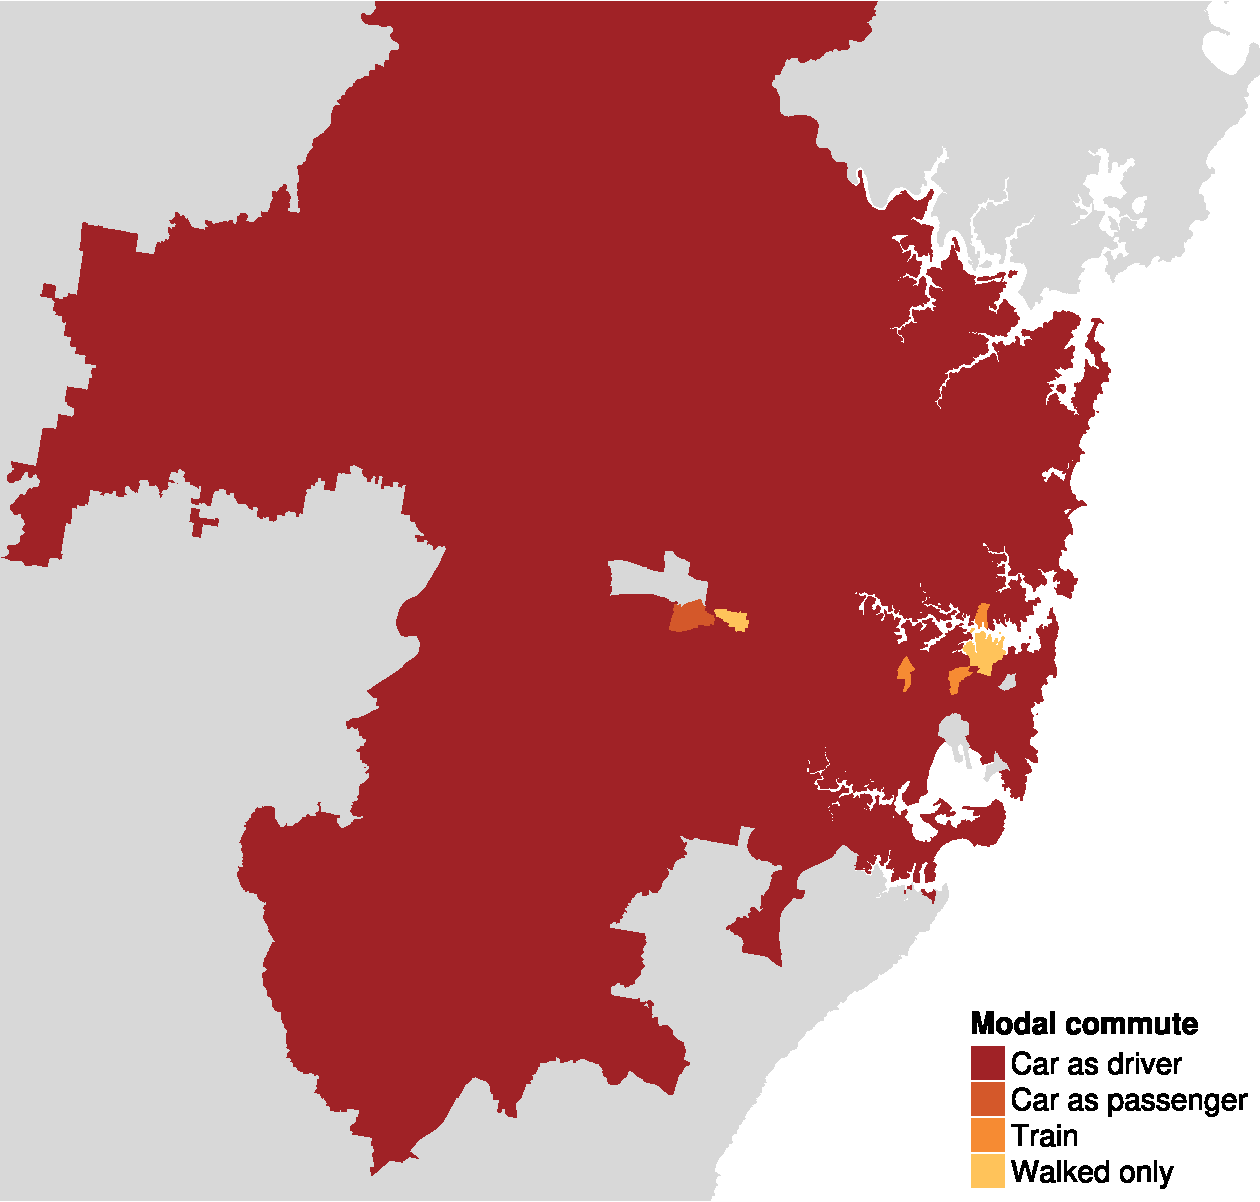
\includegraphics{atlas/Main-mode-of-transport--Sydneya-1-crop.pdf}
\noteswithsource{`Modal commute' is defined as the means that most respondents in an area used to get to work on Census day in 2011. It excludes those who did not travel to work or worked from home.
Suburbs (SA2s) outside Sydney shown as grey.}{\textcite{ABS2011Census}.}
\end{figure}

Urban Australians' car dependency can be seen in the forecast impacts of the Melbourne Metro rail project -- one of the largest public transport projects in the nation's history.%
    \footcite{MelbourneMetro-2016-BizCase}
Many more people who work in the employment precincts around Melbourne Metro's five new train stations are expected to commute by public transport.%
    \footcite[][166--167]{MelbourneMetro-2016-BizCase}
But the project is expected to have minimal impact on public transport's share of total travel across Melbourne as a whole. By 2031, public transport trips in the morning peak are forecast to increase by just 2 per cent as a consequence of the project, and car trips are expected to decline by just 0.5 per cent.%
    \footcite{Urbanist-2016-Melb-metro-What-do-you-get-for-10bn}

Whether per capita road use continues to decline or stabilises,
\footcite[][9]{BITRE-2015-Traffic-and-congestion-cost-trends-for-Aust-capital-cities}
fast-growing urban populations will mean total kilometres of road travel will continue to grow strongly in coming years.

\section{Cities adapt}

As cities become denser and more developed, it becomes more difficult to add physical capacity to a road network, for two reasons.
First, building major roads in developed areas can be astronomically expensive, and second, such roads would sometimes destroy the very character that made everyone flock to an area in the first place.

But cities adapt; the populations of cities such as New York and London have continued to grow long after the road space was fixed, yet the roads have continued to function.
Rather than spend longer commuting, people change where they live, where they work, or what mode of transport they use to get to work. In fact, the amount of time people spend travelling to work has been remarkably stable over time: up to 35 minutes each way, each day.%
    \footnote{This phenomenon is known as Marchetti's Constant from \textcite{marchetti1994anthropological}, and has also been attributed to \textcites{Zahavi-1979-UMOT-Urban-interactions}{Zahavi-1981-UMOT-Urban-interactions}.}
At the same time, businesses and employers change where they locate, so they are within reach of their workers and customers.

\section{Our fresh look at congestion}\label{sec:Our-fresh-look}

The world is not short on research and conjecture about road congestion.
But what has changed is the ever-expanding possibilities created by big data.
This report aims to contribute to our understanding of congestion and how to manage it by bringing the insights available from a very large and powerful data set.

In the chapters that follow, we rely on analysis of more than 3.5 million observations of travel duration and speeds for specific trips in Sydney, Melbourne and Brisbane, made available through Google, as described in \Chapref{chap:appendix-notes-on-sample}.
The data set was built from queries of estimated travel time for a core bundle of 350 core routes, with 25 observations collected each day between March and September 2017 in the three cities (as detailed in \Chapref{chap:Routes-sampled}).%
    \footnote{Origin-destination pairs, rather than routes, were entered into Google Maps and the travel time recorded for the fastest route between the pairs at each point in time.}
Routes in the sample were chosen to broadly reflect the type of travel that takes place in large cities.%
    \footnote{These routes were confirmed as representative by state government agencies responsible for managing the road network.}
The routes include commuting routes to and from the CBD and major employment centres, important freight routes, shorter trips within the inner, middle and outer rings, and cross-city trips.

The following chapter outlines three common perspectives on congestion and what they each tell us about the state of play -- at a city-wide level, just how concerned should we be about congestion?





\chapter{How bad is congestion in Australia's major cities?}\label{chap:state-of-play-Australia}

Roads are ``congested'' when the number of vehicles using them causes unacceptable levels of discomfort and delay.%
    \footcite[][93]{Falcocchio-and-Levinson-congestion-a-concise-guide}
But of course ``unacceptable'' means different things to different people. Motorists see aggravation. Economists see costs. Engineers look at whether the traffic exceeds a road's physical capacity. Each of these three perspectives (set out in \Cref{box:three-perspectives}) can help policy makers understand the extent and consequences of congestion.

This chapter looks at Sydney and Melbourne in 2017, to explore whether their roads are too congested, or on the way to becoming so, and how costly this is.

We show why motorists and economists believe the roads are congested. We outline why economists think the costs of congestion are very high, despite the difficulty of estimating these costs with precision. And we explain how the engineering perspective offers a window into the extent to which we should be concerned. Finally, in \Cref{sec:a-path-through}, we suggest how the three perspectives should be combined to help us understand what ``excessive'' congestion is.


\section{Motorists in Sydney and Melbourne are badly delayed during peak period trips to the CBD}\label{subsec:benchmarking-against-other-cities}

Conventional wisdom holds that Sydney is much more congested than Melbourne.
    \footcite{OSullivan-2017-Sydney-is-congestion-capital-of-Australasia}
But our examination of trip delays in the two cities reveals striking similarities.

\begin{verysmallbox}[!hp]{Defining congestion -- three perspectives}{box:three-perspectives}
%\relax
%\setlength{\parskip}{5pt plus 1pt minus 1pt}
%\relax
For \textbf{motorists}, a road is too congested if their speeds drop too far and their trip takes too much longer than expected.
In other words, motorists' perspective of congestion is about how long it takes to get from place to place, and how reliable that trip is.
Trip time and reliability are useful metrics for policy-makers when comparing congestion across cities of similar sizes, where the trip length and the number of people affected are comparable.

\textbf{Economists} focus on the costs and benefits that road users experience at different levels of traffic flow.
They pay particular attention to the difference between the private cost of an additional trip and the social cost of that trip.
\Vref{box:explaining-congestion-as-negative-externality} provides a stylised explanation of the harm to the community when the private cost of a trip is less than the social cost. In such situations, congestion reduces the economic welfare of society overall.

\textbf{Engineers}
consider a road congested when more vehicles are attempting to use the road than it has physical capacity to carry.
Capacity refers to the maximum number of vehicles the road is capable of carrying over a fixed period – the maximum possible throughput.
A road is at its carrying capacity if adding one more vehicle results in reduced rather than increased throughput.
This phenomenon, known as ``flow breakdown'', is rare in Australia.

{\footnotesize\itshape \Chapref{chap:appendix-defining-congestion} contains further details about each perspective.}
\end{verysmallbox}


In both cities, the morning peak occurs around 8\,am and the afternoon peak around 5\,pm.
If anything, delays on CBD-bound trips are higher in Melbourne than Sydney.
A comparison of CBD commuting trips (\Vref{fig:aggregate-delay-CBD-commutes}) encompasses not only those going to and from work in the city by car, but also all the delivery trucks and vans, tradespeople, workers travelling to jobs outside the CBD, students and shoppers swept up in the same traffic.
In the morning peak, the average CBD-bound trip in Sydney takes 70 per cent longer than it would in the middle of the night, but around 80 per cent longer in Melbourne.

\begin{figure}
\caption{Congestion on CBD commuting trips is very similar in Sydney and Melbourne}\label{fig:aggregate-delay-CBD-commutes}
\units{Increase in travel time relative to free flow}
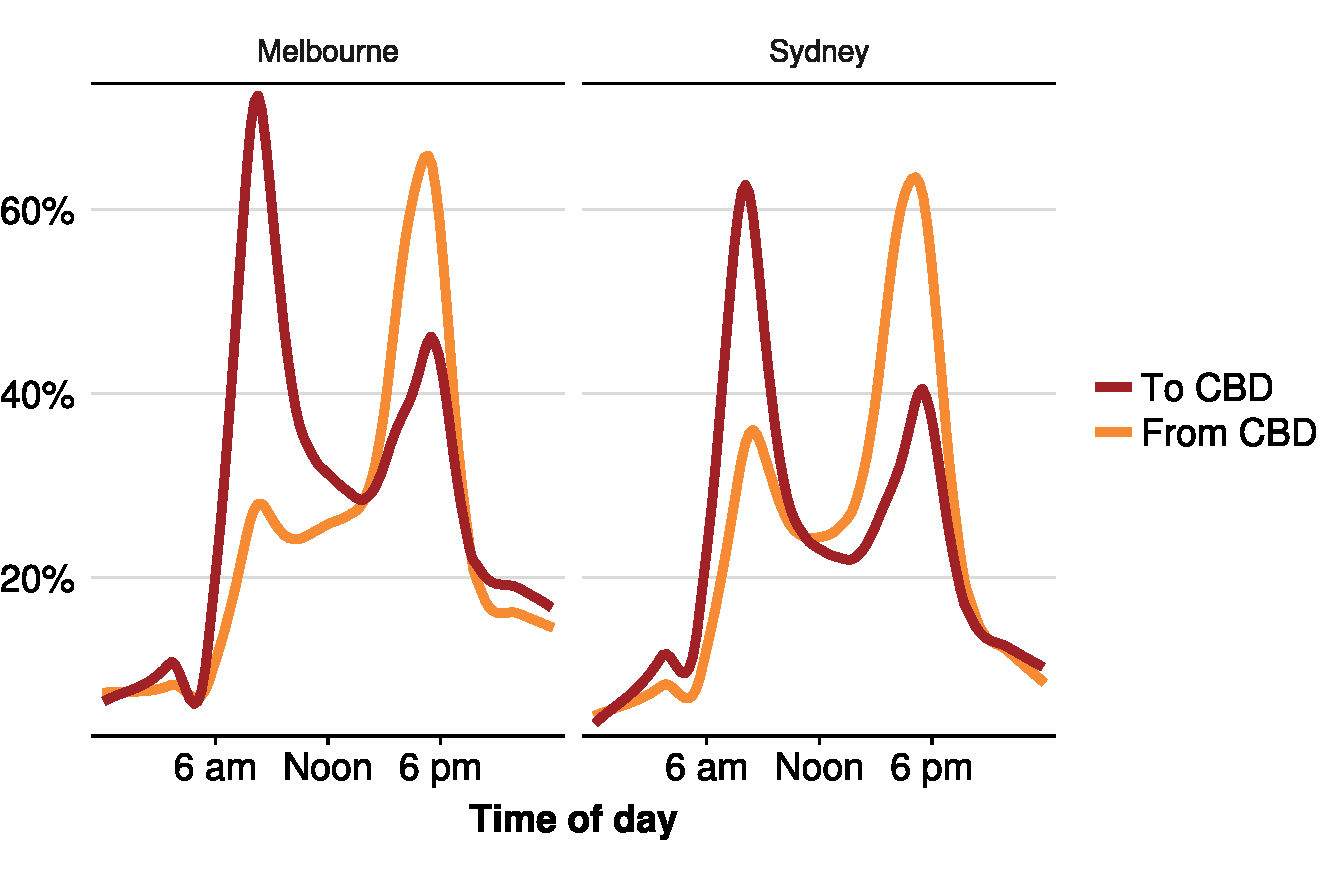
\includegraphics{atlas/CBD-commutes-time-of-day-1.pdf}
\noteswithsource{Average delay is calculated as the ratio of trip duration at each point throughout the day to the minimum trip duration observed for that route over the sample period. Details of routes used here are available in \Chapref{chap:Routes-sampled}}{Grattan analysis of Google Maps.}%
\end{figure}
\begin{figure}
\caption{The variability of CBD commuting trip times is very similar in Sydney and Melbourne}\label{fig:aggregate-variability-CBD-commutes}
\units{Increase in travel time relative to free flow, morning and afternoon peaks}
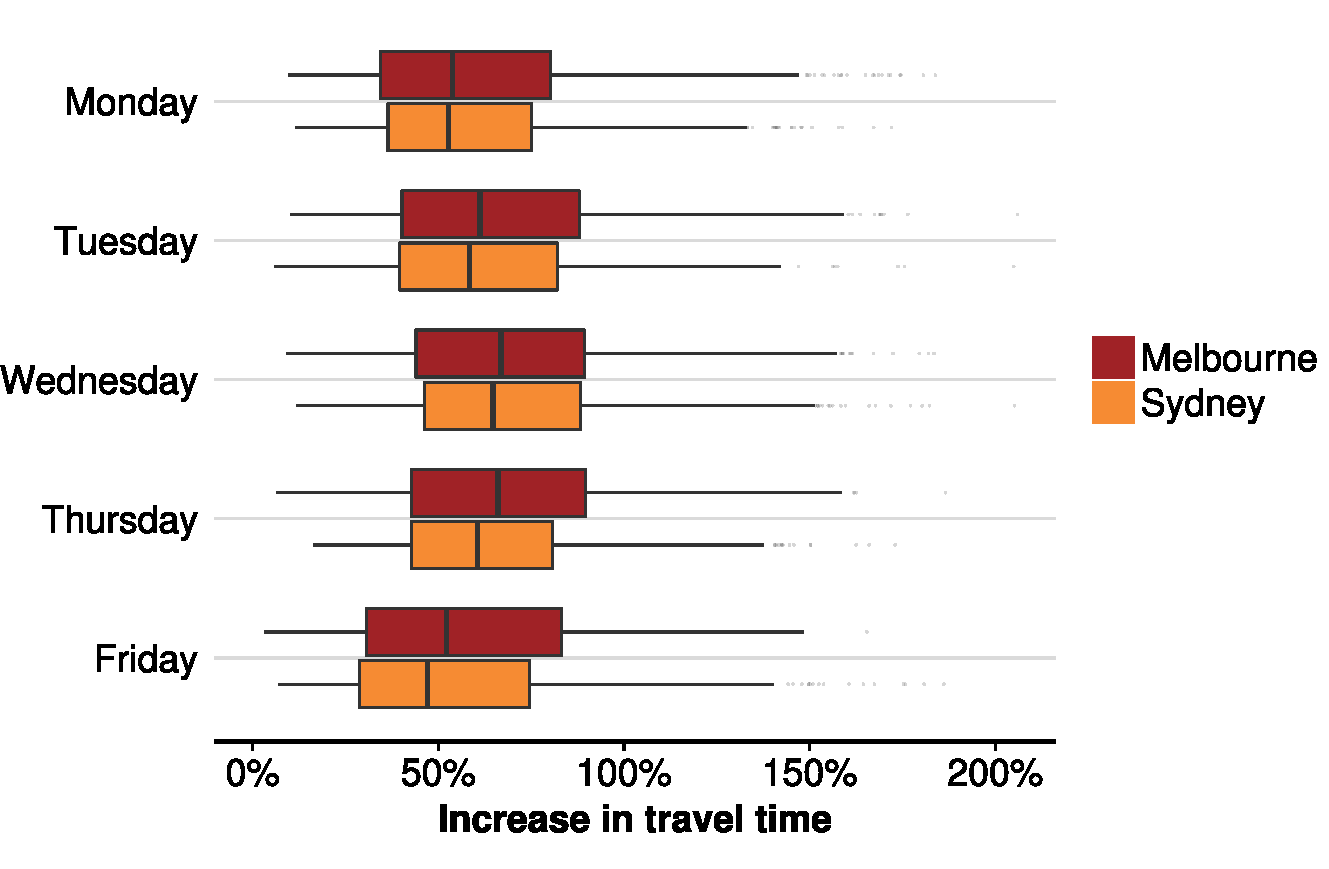
\includegraphics{atlas/boxplot-increase_in_travel_time-by-City-Weekday--MonFri-excl-holiday-1.pdf}
\noteswithsource{Only the maximum trip times for each route-day-am/pm combination are included in this chart.
The boxes cover the 25th to 75th percentiles.
The vertical line in each box lies at the median for each city.
The `whiskers' on each side of the boxes extend no further than \(\pm1.5w\) where \(w\) is the box width.
Observations beyond the lines are plotted as dots. (\textcite[][`Box Plot Statistics']{R-grDevices}.)
}{Grattan analysis of Google Maps.}
\end{figure}

The reliability of travel time for CBD commutes is also similar in Sydney and Melbourne (\Vref{fig:aggregate-variability-CBD-commutes}), although Melbourne tends to be a bit more variable than Sydney. Reliability determines how big a buffer people need to leave to ensure they get to their destination on time. Studies increasingly show that reliability of travel time is more important to road users than the typical or expected delay.%
    \footcites{2005-Small-estimates-for-travel-time-and-reliability}{2017-Brent-and-Gross-value-of-travel-time-and-reliability}{Cortright-2017-CityObs-What-hot-lanes-reveal-about-the-value-of-travel-time}


\section{The economic costs of congestion are very large}\label{subsec:economists-think-costs-are-very-large}

The main drawback of the motorist's perspective is the absence of a threshold by which we can objectively assess the costs of congestion. The perspective of economists is helpful here -- it explains why the delays and variability we observe in \Cref{fig:aggregate-delay-CBD-commutes} and \Cref{fig:aggregate-variability-CBD-commutes} are concerning, and how they can be quantified.

Economists seek to measure the avoidable social costs of congestion -- the costs that can, in principle, be saved through measures to address congestion.
They capture how much time and fuel could be saved, and air quality improved, if travel volumes were reduced to the socially optimal level.
This optimal level of travel is defined as that which would result if road-users took into account not only their personal costs, such as time and vehicle-operating costs, but also the costs they imposed on other road-users through their contribution to overall congestion. A stylised example showing how personal and social costs diverge is set out in \Vref{box:explaining-congestion-as-negative-externality}.

Estimates of the costs of congestion using the economist's framework tend to be huge and headline-grabbing -- and often misused (\Vref{box:mis-use-of-economic-cost-estimates}). The Bureau of Transport, Infrastructure and Regional Economics (BITRE) says congestion is costing \$6.1~billion a year in Sydney and \$4.6~billion a year in Melbourne, and these costs are projected to more than double by 2030.%
    \footcite[][1]{BITRE-2015-Traffic-and-congestion-cost-trends-for-Aust-capital-cities}
Infrastructure Australia (IA) says that congestion cost \$5.5 billion in Sydney and \$2.8 billion in Melbourne in 2011, with these costs projected to increase to \$14.8~billion and \$9.0~billion respectively by 2031.%
    \footnote{While IA's specific methodology is not published, some details can be found in \textcite[][379--393]{Acil-Allen-report-for-Infrastructure-Australia-National-Infrastructure-Audit}.}

BITRE's and IA's estimates have been important in highlighting to the public that congestion is not just aggravating but costly.

But the economist's framework has its limits:

\begin{itemize}
\item  \textcite{BITRE-2015-Traffic-and-congestion-cost-trends-for-Aust-capital-cities} acknowledges that ``such aggregate -- citywide averaged -- methods are very blunt instruments for estimating and projecting congestion occurrence''.
    \footcite[][15]{BITRE-2015-Traffic-and-congestion-cost-trends-for-Aust-capital-cities}
\item Measurement using the economic perspective requires big assumptions about what costs are avoidable. In practice, the rule of thumb is to assume that half of the difference between travel time costs at free-flow speed and those at the current average speed can be avoided.%
    \footnote{``DWLs [the avoidable costs of congestion] appear to be in the order of half total delay costs for typical peak traffic conditions -- where their proportion would be much lower for light traffic and grow rapidly for severely congested areas'':
    \textcite[][78]{BITRE-2007-Estimating-urban-traffic-and-congestion-cost-trends}.}

\end{itemize}

\begin{smallbox}{Estimates of the economic costs of congestion are misused and poorly understood}{box:mis-use-of-economic-cost-estimates}
Frequently, commentators mistakenly assume that the costs of congestion as estimated by BITRE are translatable directly into larger economic output or even government revenue.
Recent examples of this include:

\microtypeforquote
\begin{quote}
\textquotedblleft Imagine if each and every year, the Australian Government discovered a hollow log containing \$16.5~billion. We could use that windfall to boost services or reduce government debt. Or we could return the money to the pockets of families and small businesses via tax cuts. Actual hollow logs are rare in Canberra.''%
    \footcite{Albanese-2017-Congestion-handbrake-on-growth}

``Nationally, the urban congestion debt that is currently robbing the economy of more than \$16.5 billion a year is set to soar to around \$30 billion by 2030.''%
    \footcite{Chester-VTA-2017-Freight-speech}

\end{quote}

Few acknowledge that mitigating congestion is not costless. For example, if a road-pricing scheme were used to reduce traffic volumes so that the estimated benefits materialised, this would require funds for implementation, new infrastructure and ongoing administration. BITRE itself cautions that the estimated costs of congestion ``do not directly refer to actual obtainable savings for congestion reduction measures, since the introduction and running costs will vary from measure to measure (and in some cases will be considerable)".%
    \footnote{BITRE, 2015, page 19.}
\end{smallbox}

The key contribution of the economists' perspective is that it offers a framework for understanding the costs of congestion beyond the direct costs faced by each individual driver. While unsuitable for policy design purposes in their present form, we are optimistic that, in time, and with the ever-expanding possibilities of big data, economic cost measures will play a greater role in the understanding and management of congestion. 

\section{Engineers will tell you that few roads are congested beyond their physical capacity}\label{subsec:quantifying-capacity}

Engineers give us a different take on congestion, because they are most concerned about the carrying capacity of the roads.

Engineers measure a road's Level of Service (or LOS) on a scale from A to F, where A is free-flowing traffic and F is flow breakdown.%
    \footcite[][Part~3: Traffic Studies and Analysis, p.~63]{Austroads-2015-Guide-Traffic-Mgmt}
This perspective is helpful in providing a snapshot of the overall performance of our roads. If we see that roads are regularly in a state of flow-breakdown, then it is clear that solutions need to be identified urgently. Alternatively, if we see that roads rarely experience anything other than free-flowing traffic, then we would have reason to consider the problem trivial or non-existent -- and to direct policy makers' attention away from the problem of congestion altogether.

Perhaps unsurprisingly, neither of these situations describes the state of play in Sydney and Melbourne, where arterial roads generally operate somewhere between flow-breakdown and free-flow. In some of the most congested inner-suburban corridors, travel flow is, on average, very good for most of the time on an average day
(see \Vref{fig:LOS-innersuburb-SYD}).
Even on the worst weekday in a typical week, peak-hour traffic flows are still stable, with most roads providing a LOS better than D.%
    \footnote{"Level of Service D indicates a less stable condition in which small increases in flow may cause substantial increases in delay and decreases in travel speed\dots{} The travel speed is between 40\% and 50\% of the base free-flow speed'': \textcite[][Part~3, p.~63]{Austroads-2015-Guide-Traffic-Mgmt}.}

\begin{figure*}
\begin{minipage}[t][\textheight]{\columnwidth}
    \captionsetup{oneside, margin={0em,-25em}}%
    % HP: Switching cities is a bit more work. Straigtforward to do but I'll wait till we know where this chart is going.
	\caption{Even on notoriously congested short routes, average levels of service remain good most of the time}\label{fig:LOS-innersuburb-SYD}
	\units{Travel speed as a proportion of free-flow travel speed, and level of service category, non-freeway routes, Sydney and Melbourne}
	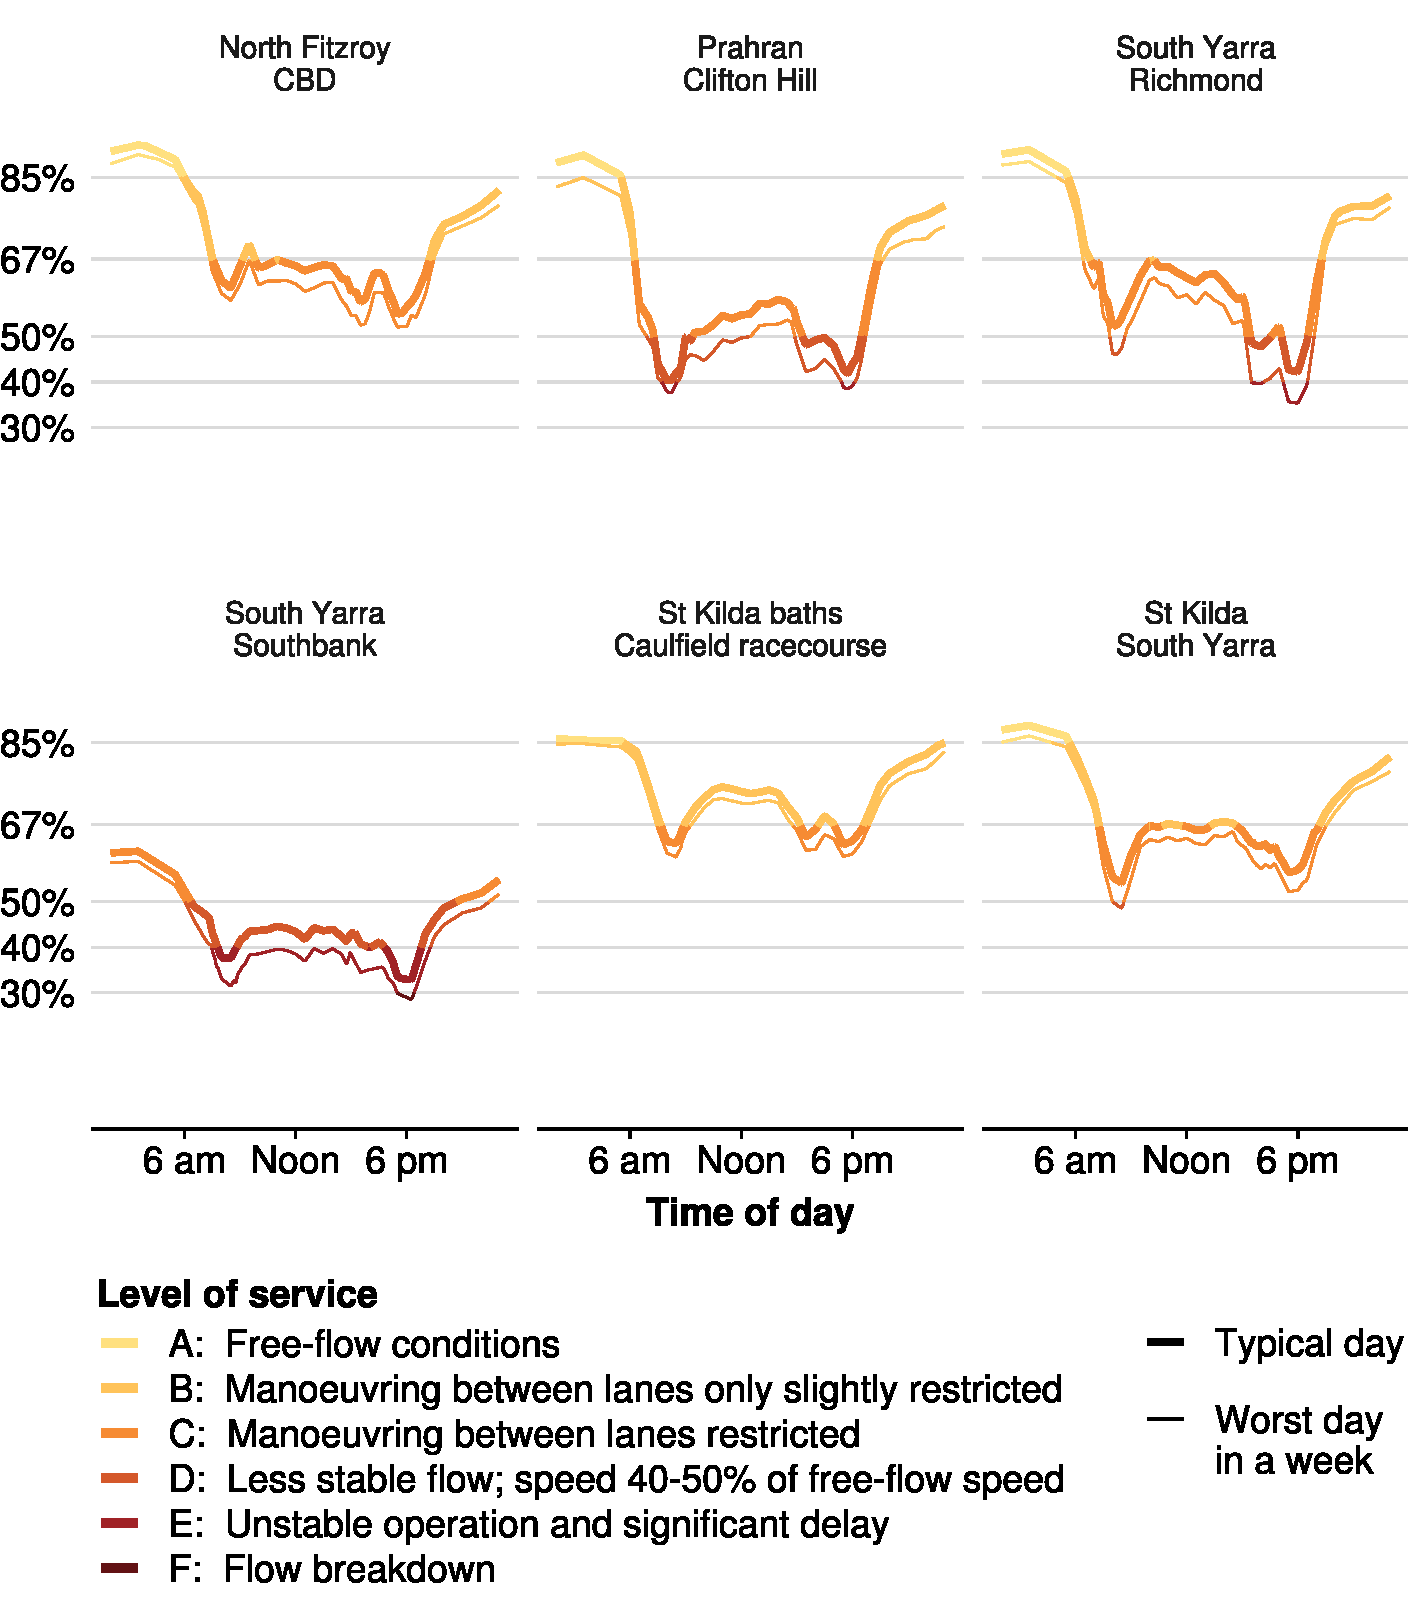
\includegraphics[width=1.06\columnwidth]{atlas/Avg-LOS-short-routes-MEL-1.pdf}
	\notewithsource{Free flow speed is the fastest observation captured for each route during the sampling period}{Grattan analysis of Google Maps, and \textcite[][Part~3: Traffic Studies and Analysis]{Austroads-2015-Guide-Traffic-Mgmt}}
\end{minipage}
\hfill
\begin{minipage}[t][\textheight]{\columnwidth}
  \caption*{\null}
  \units{\null}
  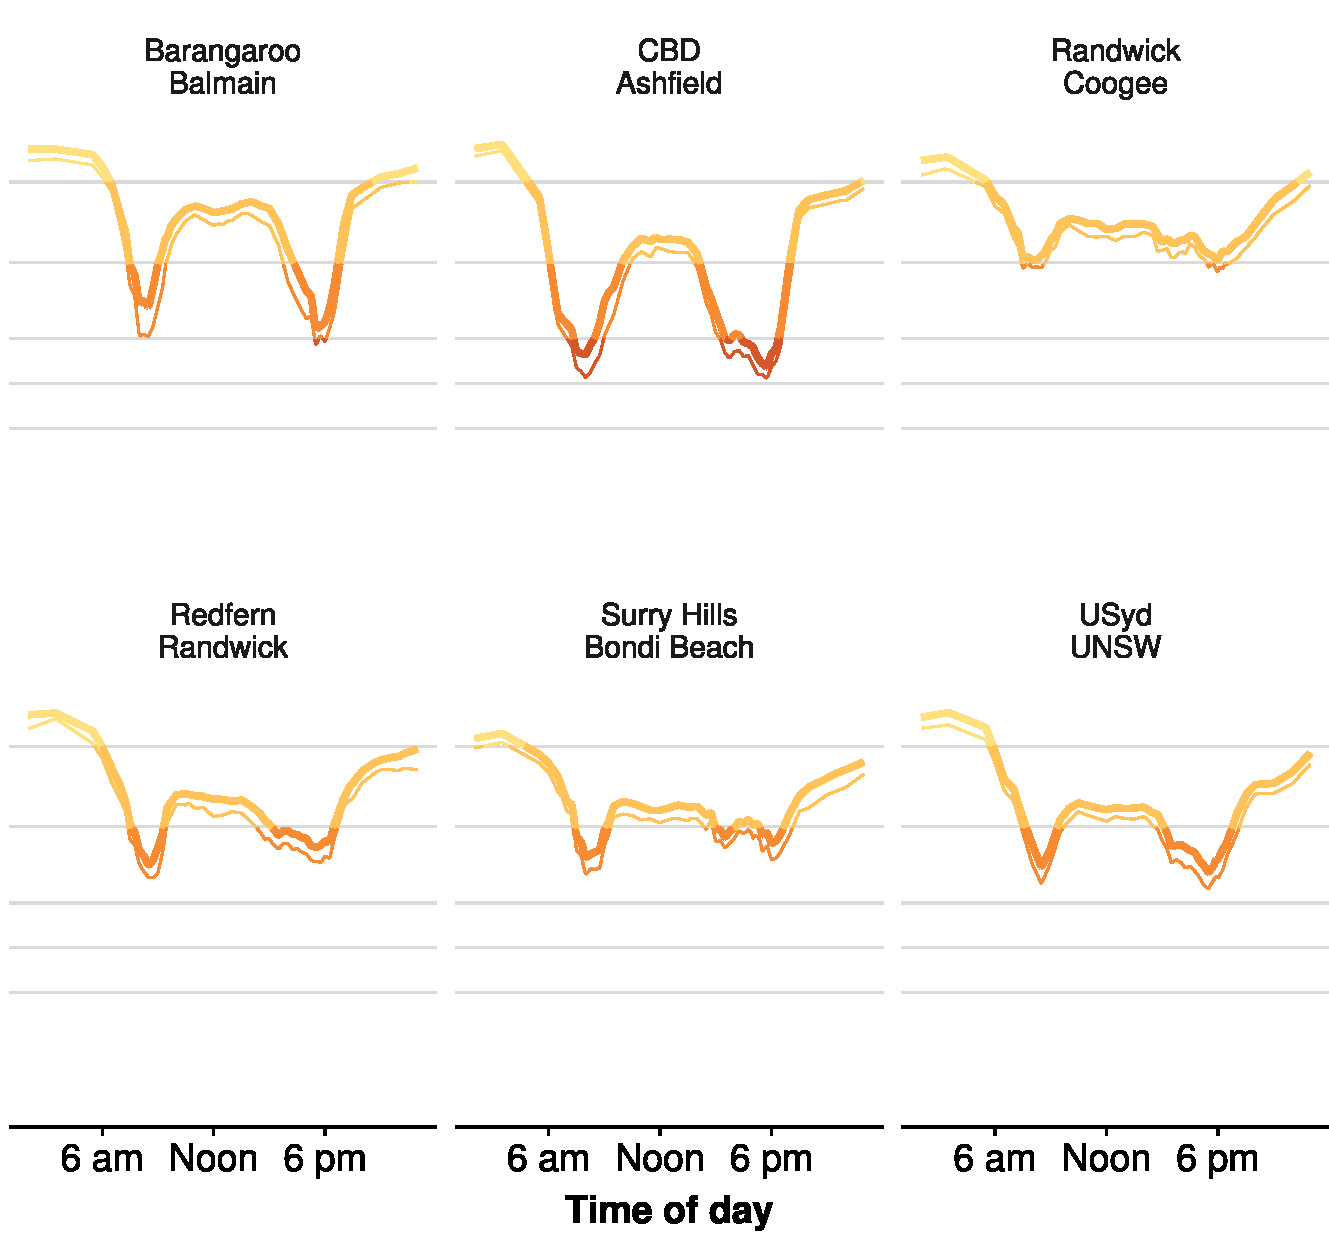
\includegraphics{atlas/Avg-LOS-short-routes-SYD-1.pdf}
  \null\vfill\null
\end{minipage}
\end{figure*}

Some urban freeways appear to have very high delays with less stable traffic flows. Average speeds on Melbourne's inner-suburban freeways have fallen below 50 kilometres per hour during the morning peak period since 2010 (see \Vref{fig:speed-Vic-freeways-vs-year}). In contrast, Melbourne's middle and outer-region urban freeways appear to have much more stable traffic flows,%
    \footcite{Vicroads-201415-TravelSpeed-tableau}
although detailed time-of-day analysis is not available for urban freeways.%
    \footnote{Public data showing delays on freeways at different times of day is not available. Our own data set is also not well-suited to assessing the level of service on freeways, because it requires the use of precise postal addresses as origins and destinations, which do not exist for freeway segments.}


\section{Identifying ``excessive'' congestion}\label{sec:a-path-through}

This chapter has shown that how bad you think congestion is depends on your perspective, and how costly you think it is depends on how you measure the costs. Each perspective is based on sound principles and contributes to an understanding of congestion, but each also has its drawbacks. For example:

\begin{itemize}
\item The motorists’ perspective lacks an explicit benchmark for determining the point at which congestion is excessive.
\item Precise measurement of the economists' perspective on costs is difficult. Even so, this view is an important complement to the motorists' perspective, with its focus on individual costs and delays, as it provides a framework for understanding the costs of congestion to society as a whole. 
\item The engineers' perspective provides a benchmark for when a road exceeds its carrying capacity -- but it does not capture the aggravating delays and unreliability, and the costs of such delays, that concern motorists and economists well before flows break down.
\end{itemize}

Despite these limitations, we are still able to get a good sense of ``excessive'' by combining the underpinning principles of the economists’ perspective -- that delays are costly, and they arise because motorists do not consider the full costs of their travel decisions -- with our measures of delays and variability from a motorist's perspective.

On any view, the extent of congestion and its costs -- and the value of reducing it -- varies from time to time and from place to place. In certain places and at certain times, congestion poses real social and economic costs that governments should be actively addressing.

The next two chapters focus on the motorists' and the economists' points of view.
To understand how we can identify causes and solutions in Sydney and Melbourne, a more detailed analysis of each city is required; an examination of the magnitude of congestion in different parts of the city at different times of the day and week.

\begin{bigbox*}{What do economists really mean when they talk about the social costs of driving?}{box:explaining-congestion-as-negative-externality}

When economists refer to the social costs of driving (see \Cref{subsec:Economists-perspective}) they are pointing to costs beyond those borne by the individual driver.
When a driver decides to take a trip, above and beyond the private costs and benefits of that trip, the broader community can pay a price through congestion.

To understand this better, let's think about a particular situation.

Imagine a person who commutes from home to work each weekday.
During the morning peak, her trip takes around 60 minutes.
So she knows that to reach the office by 9\,am she needs to be in the car by 8\,am.

For simplicity, let's assume the entire trip is on a freeway, and there is a single set of traffic lights at the end of the freeway at which motorists regularly spend 30 minutes waiting to get through on any given morning.

Why would she do it? Clearly, when she thinks about the costs and benefits of travelling by car versus alternatives such as travelling by train or driving  earlier in the morning before the rush, the benefits outweigh the costs.
But while the benefits might outweigh \textit{her} costs, economists emphasise the costs she imposes on other motorists by making congestion that little bit worse.

The best way to see these congestion costs is to imagine removing her trip.
If she was at the front of the traffic-light queue, removing her from the stream of traffic makes it possible for a car that would otherwise have had to wait for another light cycle to make it through.
If the light cycle takes one minute, then removing her one vehicle has reduced congestion by one-minute for one other motorist.

But the impact doesn't end there – with the line of cars now one fewer than it was before, at the following light change it is again possible for an additional driver to make it through, saving one more minute for one more motorist.
The time savings will continue for as long as the congestion lasts.
If the original motorist is removed when there is one-hour of congestion left, then there is a saving of 30 minutes of time for other drivers – one minute at 30 changes of lights (if we assume that the lights go red for one minute, and green for the next minute).

Our motorist might think of herself as “just one more car”, but the costs she imposes on other drivers are significant.
If we value people's time at \$20 an hour, just those 30 minutes has imposed additional “social” costs of \$10 that were not considered when the original private travel decision was made.

If this trip is assumed to be representative of all trips, then a rough rule of thumb for the economic costs of congestion would be to multiply the \$10 estimated social cost of a trip by the total number of trips during the morning peak.
The economists' point is clear: the costs individual motorists impose on the broader community, and which they often do not even consider, are likely to be large.

\boxsources{\textcite{King-and-Gans-Finishing-the-Job}}
\end{bigbox*}










\chapter{Where and why is congestion a problem in Sydney?}\label{chap:Congestion-Sydney}

Sydney and Melbourne have similar congestion when viewed from a city-wide perspective, but different congestion-management policies.
To develop better policies to ease congestion in each city,  a better understanding is needed of exactly where and when congestion is most acute in each city.

The first part of this chapter shows that congestion varies across different parts of Sydney.
In many places it barely registers, but it can be acute across the CBD and the inner suburbs.

The second part of the chapter identifies causes of congestion in Sydney.
The most important appear to be the wide span of Sydney's centre, its topography, limits to the coverage and capacity of its rail network, and the lack of coordination of its extensive (and growing) toll road network. The chapter concludes with a look at non-recurrent causes: rain and accidents.


\section{Congestion varies greatly across Sydney}

Commuters to Sydney's CBD often endure heavy congestion. But this is not the typical experience for all road users. In many areas of Sydney, particularly outer regions where a large proportion of the population lives and works, the typical commuting delay is minimal.%
    \footnote{Delays are calculated as the additional minutes spent in traffic compared to travelling in free-flow conditions, such as usually occurs very late at night.}

\begin{figure}
\caption{For many Sydney commuters, congestion is very modest, rarely more than 5~minutes longer than if there were no traffic\dots{}\label{fig:congestion-not-significant-for-many-users}}
\units{Additional minutes compared to free flow, journeys to work, Sydney}
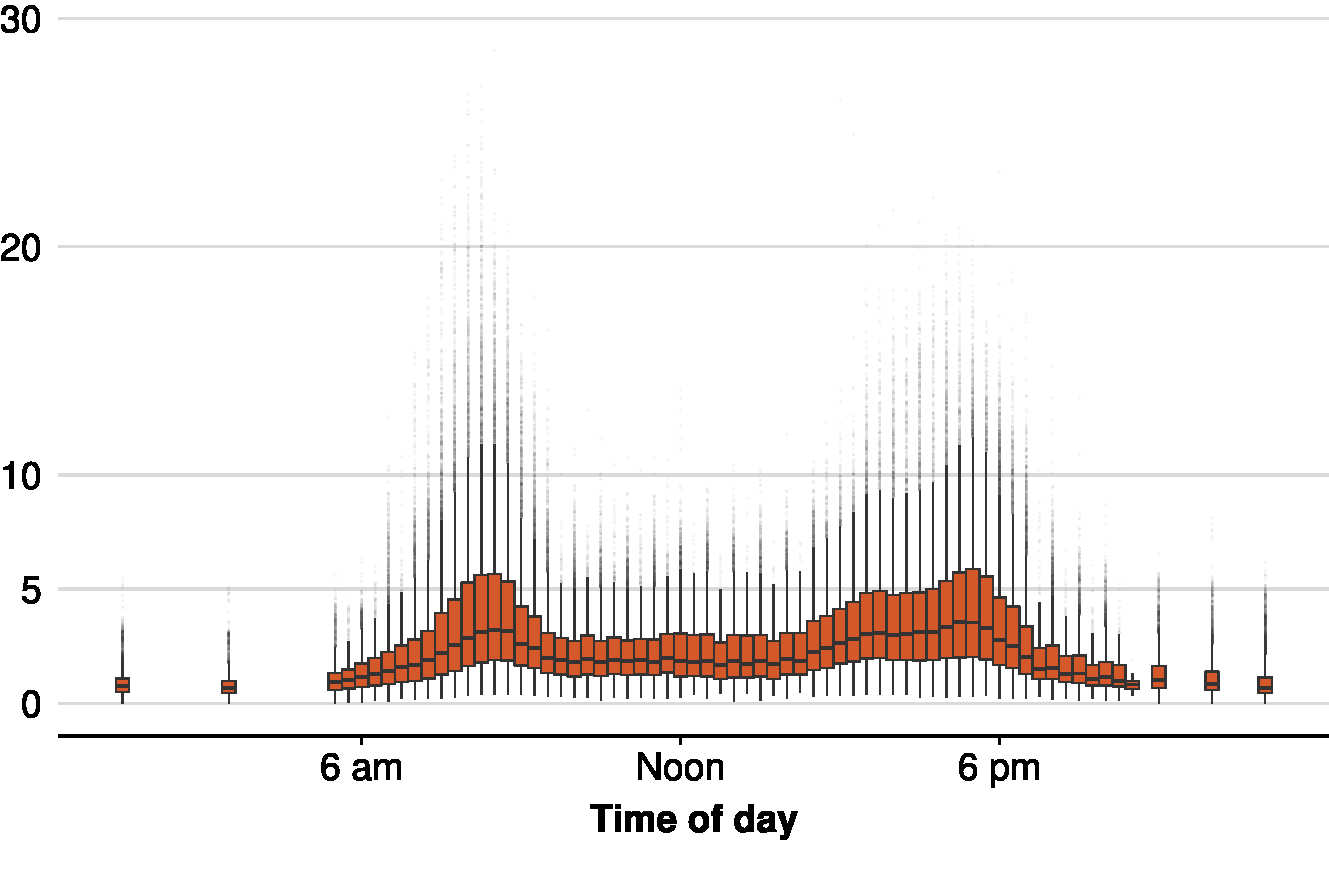
\includegraphics{atlas/Sydney-SA2-extra_minutes-vs-time_of_day-1.pdf}
\noteswithsources{The horizontal black line in the coloured bar is the median of all journey-to-work routes, weighted by the number of people who used a car to travel to work on those routes in the 2011 Census reference week.
Trip times were estimated by assuming all travel between suburbs was between representative addresses for each suburb.
Routes with fewer than 400 such commuters are not included.}{Grattan analysis of Google Maps, and \textcite{ABS2011Census}.}%
\end{figure}

\begin{figure}
\caption{\dots{} and even for commutes into the CBD in the morning peak, the average delay is just 11 minutes\label{fig:weighted-cbd-commuting-delay-sydney}}
\units{Additional minutes compared to free flow, journeys to work in the Sydney CBD}
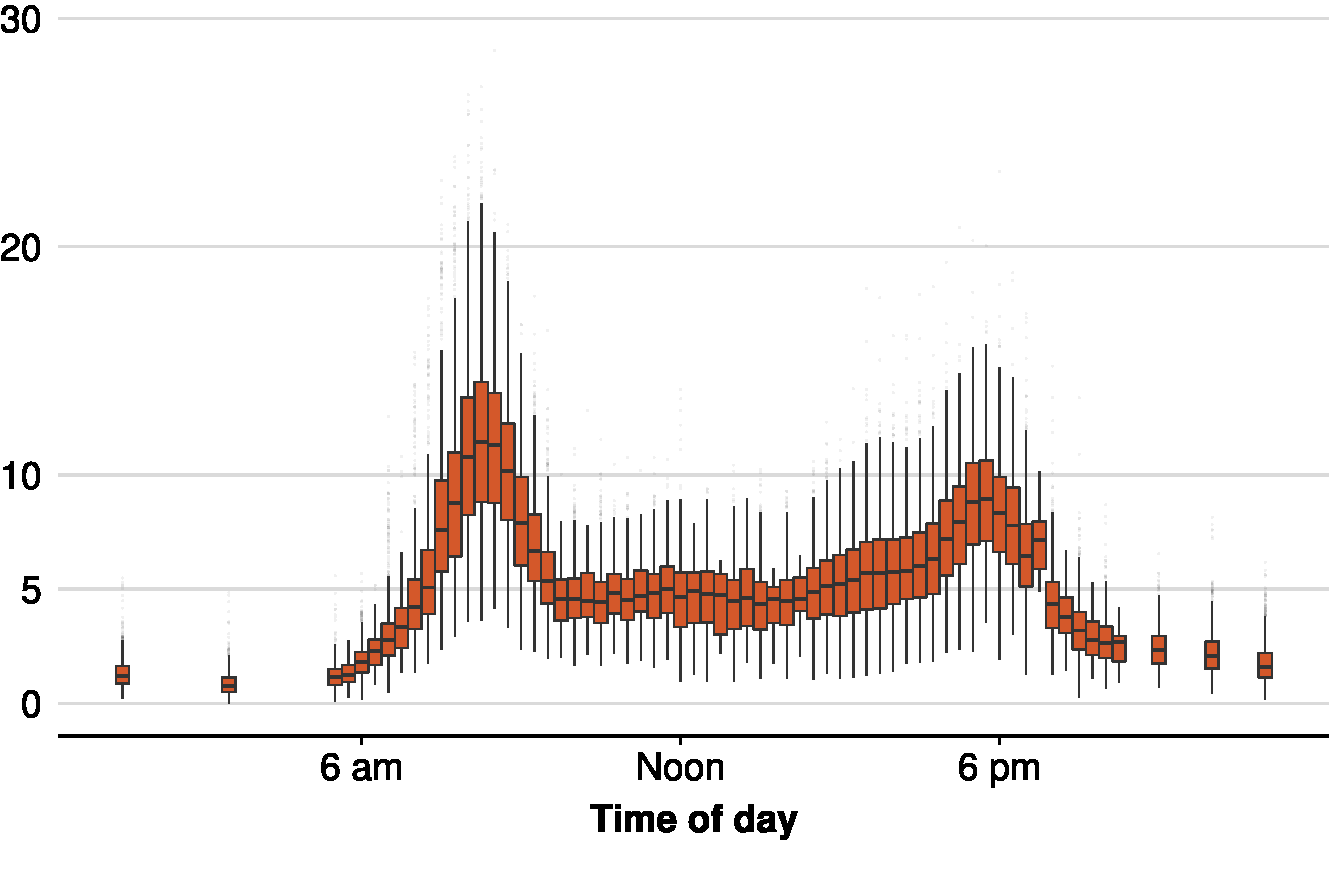
\includegraphics{atlas/Sydney-SA2-CBD-extra_minutes-vs-time_of_day-1.pdf}
\noteswithsources{The horizontal black line in the coloured bar is the median of all journey-to-work routes, weighted by the number of people who used a car to travel to work on those routes in the 2011 Census reference week.
Trip times were estimated by assuming all travel between suburbs was between representative addresses for each suburb.
Routes with fewer than 400 such commuters are not included.}{Grattan analysis of Google Maps, and \textcite{ABS2011Census}.}%
\end{figure}

\begin{figure*}
\caption{Commuters outside central Sydney typically experience only small delays \label{fig:map-Sydney-sa2-commuting-congestion-minutes}}
\units{Commutes between suburbs with more than 400 drivers}
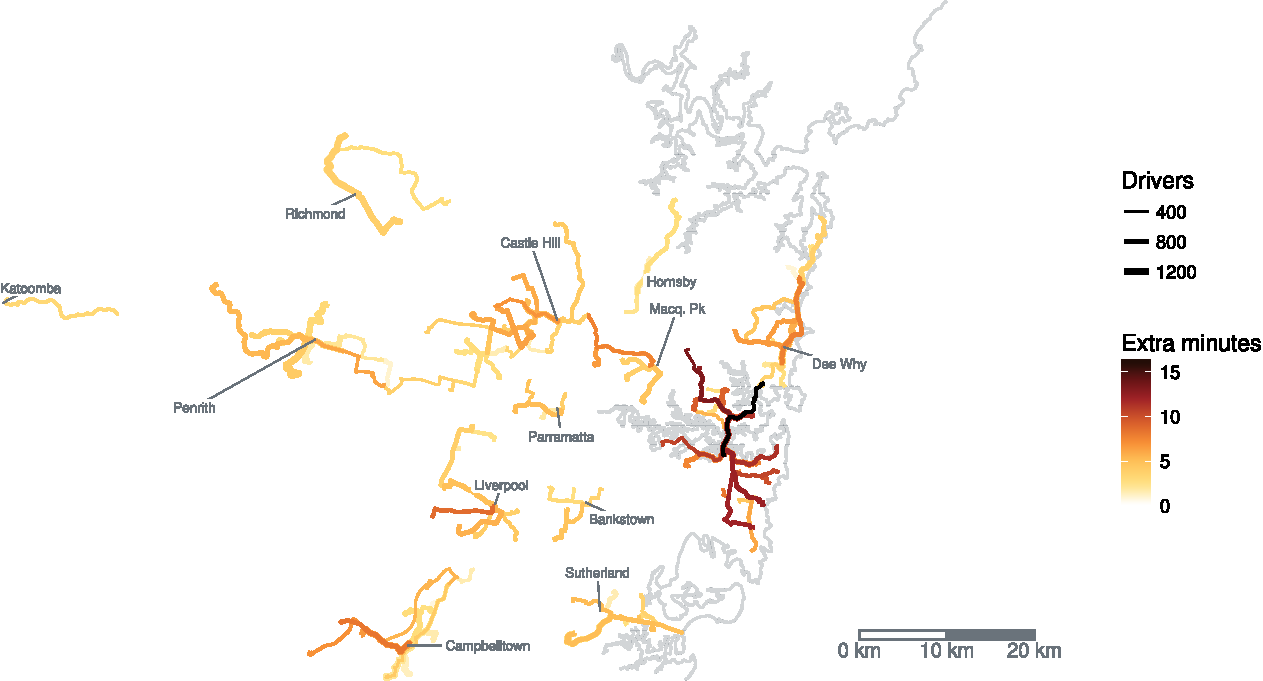
\includegraphics[width=1.9\columnwidth]{atlas/Central-Sydney-is-the-focus-of-congestion-1-crop.pdf}
\sources{Grattan analysis of Google Maps, and \textcite{ABS2011Census}}
\end{figure*}


\subsection{Most Sydney commuters experience minimal delays}

It is common to assume that commuting usually involves driving into the city.
But in Sydney 86 per cent of people travel to work somewhere other than the CBD\@.
\footcite{ABS2011Census}
Most people work in a suburb close to where they live. %
For many of them, congestion on the daily commute is minimal.

The number of minutes of delay for Sydney's 146 most common commuting trips is shown in \Vref{fig:congestion-not-significant-for-many-users}.%
    \footnote{This analysis is based on the best available data, which covers commuting routes used by more than 400 drivers.}
The delay is less than five minutes on the average commute which takes around 10 minutes in the middle of the night.
While some commuters suffer much longer delays, it is very unusual for trips to take more than 20 minutes extra in peak periods than they would in the middle of the night.

% \begin{figure}
% \caption{Trips to central Sydney have longer delays than trips to non-CBD employment centres\label{fig:cbd-and-non-cbd-commuting-delay-sydney}}
% \units{Extra delay in minutes relative to free flow of traffic}
% 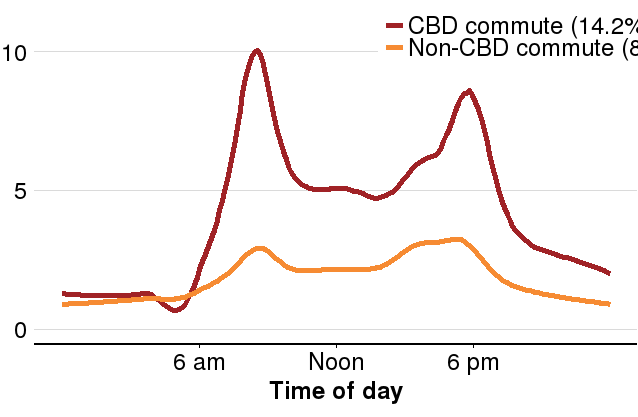
\includegraphics{atlas/extra_mins-vs-time_of_day--CBD-Non-CBD-SYD-1.pdf}
% \noteswithsource{Routes with more than 400\,drivers in 2011. See \Chapref{chap:Routes-sampled} for the full list of `Sydney SA2' routes.}{Grattan analysis of Google Maps.}%
% \end{figure}

\subsection{Congestion is worst in and around central Sydney}\label{subsec:worst-around-central-sydney}

It is unsurprising that congestion is worst in and around central Sydney. A typical delay for travel on routes to Sydney's CBD in the morning peak is around 11 minutes, but some trips appear regularly delayed by as much as 15-20 minutes (\Cref{fig:weighted-cbd-commuting-delay-sydney}).

This is presented spatially in \Vref{fig:map-Sydney-sa2-commuting-congestion-minutes}, showing that trips to the central part of Sydney are more delayed than elsewhere.



\subsection{Trip times can be unreliable right across Sydney}

Most travellers care not only about how long a trip usually takes, but also how long it \emph{could} take.
If the typical delay is highly unreliable -- if, for example, every few days a 20-minute commute takes 30 minutes -- drivers will need to incorporate this potential extra delay into their schedule.
The reliability of travel is an important determinant of its economic costs.%
\footcites{2005-Small-estimates-for-travel-time-and-reliability}{2017-Brent-and-Gross-value-of-travel-time-and-reliability}

\begin{figure}
\caption{Reliability can be a problem everywhere\label{fig:boxplot-variability-by-route}}
\units{Increase in travel time as a proportion of free flow, weekday morning peak, commutes into Sydney CBD}
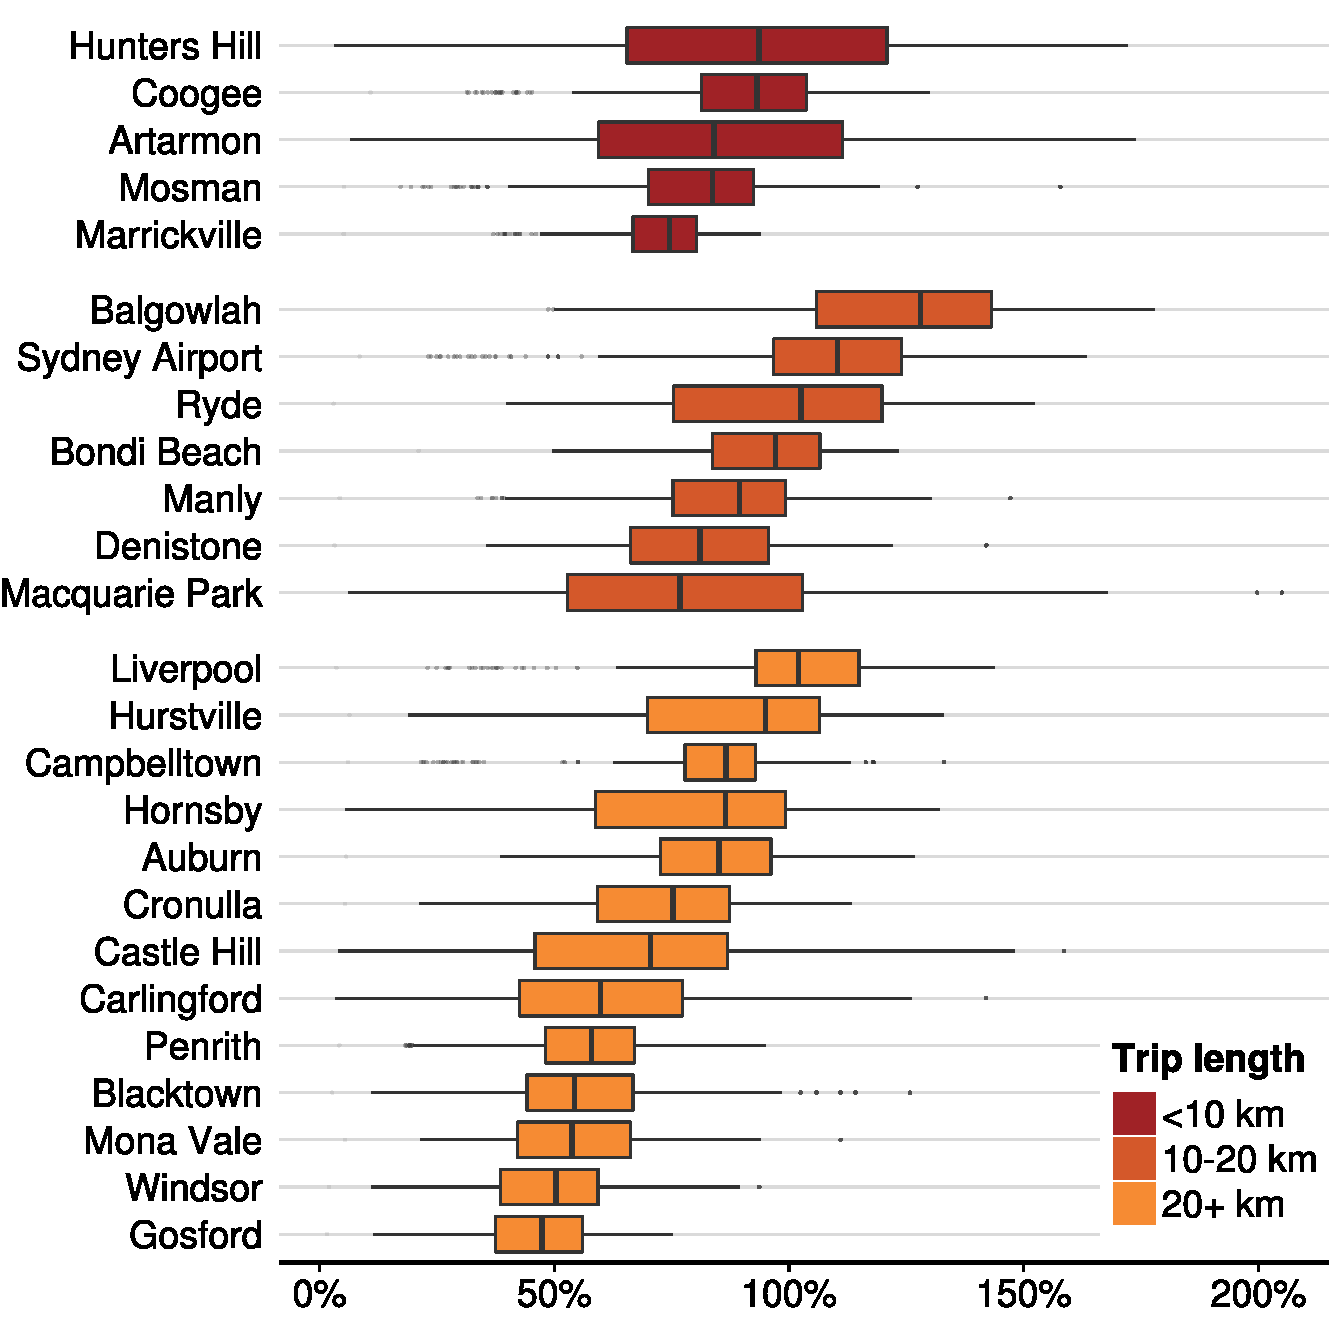
\includegraphics{atlas/boxplot-increase_in_travel_time-by-Suburb--Sydney-CBD-commutes-1.pdf}
\noteswithsource{For travel departing between 7\,am and 9\,am.
Excludes weekends and public holidays. The boxes cover the 25th to 75th percentiles. The vertical line in each box lies at the median for each city. The `whiskers' on each side of the boxes extend no further than \(\pm1.5w\) where \(w\) is the box width. Observations beyond the lines are plotted as dots.
}%
{Grattan analysis of Google Maps.}
\end{figure}

Many commutes to Sydney's CBD, whether from the inner suburbs, the middle ring or outer areas, are unreliable; some individual trips can take much longer than the typical trip on the same route, as shown in \Cref{fig:boxplot-variability-by-route}.
People on these routes need to leave a substantial buffer to get to their destination on time.


The commute from Artarmon to the CBD, for example, is very unreliable.
With no traffic this trips takes about 12~minutes. The commute at peak hour takes on average around 20~minutes, but this commute is highly variable: one day a week the trip can take just 15~minutes, and another day 25.
To avoid being late for work more than one day a month, the Artarmon commuter needs to allow 30~minutes, about 10~more than the average time in peak hour, and 18~minutes more than with no traffic.

\section{Sydney's congestion has many causes}

The next sections of this chapter highlight several key causes of Sydney's distinctive pattern of congestion: the city's extensive economic core, its unique topography, the gaps in its rail network coverage, and its large (and growing) toll road network.
The chapter ends with a look at the effects of rain and accidents.

\subsection{Sydney's centre extends much further than Melbourne's}{\label{subsec:jobs-in-sydney-are-dispersed}}
Sydney's inner and middle suburbs are much more densely populated than Melbourne's (see \Vref{fig:sydney-vs-melbourne-population-density}).
Sydney has 114 square kilometres with a population of more than 5000 per square kilometre, compared to 34 equivalent square kilometres in Melbourne, three in Brisbane, and none in any other Australian capital.%
    \footcite{Urbanist-2015-population-density-is-Sydney-an-outlier}

Sydney also has more concentration of economic activity in its centre, as shown in \Vref{fig:sydney-vs-melbourne-employment-density}. And this high concentration of economic activity extends over a large geographic area. In fact, the economic ``centre of gravity''%
    \footnote{\textcite[][8]{PWC-Committee-for-Sydney-centres-of-gravity-for-emp-and-pop}: ``The Centre of Gravity is where the pull of the economic, employment and residential forces within the city are evenly balanced.
    For example, in a city where there are only three small areas, each of equal distance apart and of equal economic activity, the Centre of Gravity would be in the very middle.
    If areas had different levels of economic activity, the location of the Centre of Gravity would be pulled towards areas with greater economic activity.
Sydney's economic, employment and residential Centres of Gravity are calculated based on over 230 small areas (ABS Statistical Area Level 2 geographical classification).''}
is further from the CBD in Sydney than in any other city in Australia. And while the centre of gravity is intensifying in the CBD in most Australian cities, Sydney's has for some years been moving away, westward towards Parramatta.%
    \footcite[][3]{PWC-Committee-for-Sydney-centres-of-gravity-for-emp-and-pop}

Sydney's broader spread of population and employment means that commuters into the city are more delayed when they come from the middle ring than from the inner suburbs (\Vref{fig:boxplot-variability-by-route}). 

Sydney's greater population density may also explain why there are longer delays on its key freight routes (\Cref{fig:freight-routes-syd-and-melb}). These routes include trips in and out of Sydney Airport, Port Botany and along major freight corridors.%
    \footnote{Full route details are included in \Chapref{chap:Routes-sampled}.}

\begin{figure}
\caption{Sydney freight routes are more delayed than comparable freight routes in Melbourne\label{fig:freight-routes-syd-and-melb}}
\units{Increase in travel time relative to free flow, key freight routes}
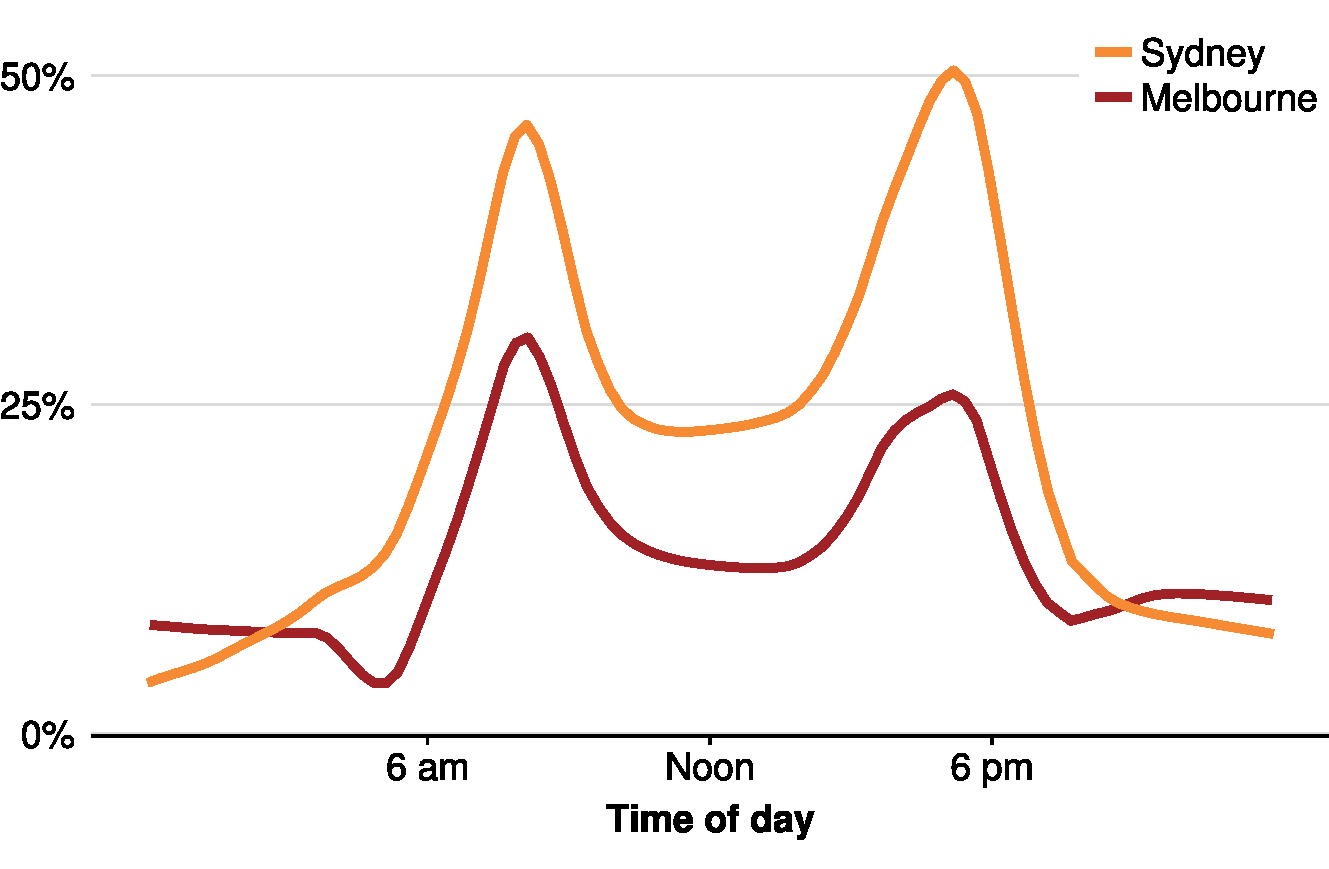
\includegraphics{atlas/increase_in_travel_time-vs-time_of_day-by-City--Freight-1.pdf}
\notewithsource{Average delay is calculated as the ratio of trip duration at each point throughout the day to the minimum trip duration observed for that route over the sample period. Details of routes used here are available in \Chapref{chap:Routes-sampled}}{Grattan analysis of Google Maps.}
\end{figure}

Freight vehicles are only a small minority of vehicles on the road, but their movement is critical to the economy. Sydney Airport is the largest import and export airport in the country, and Port Botany is second only to the Port of Melbourne for the value for merchandise imports it handles.%
   \footcite[][6]{BITRE-2014-Freightline}
The broader spread of congestion in Sydney ultimately suggests the economic costs of congestion may be larger in Sydney than Melbourne.


\begin{figure*}
\caption{Sydney's population is much denser in inner and middle areas than Melbourne's\dots{}\label{fig:sydney-vs-melbourne-population-density}}
\units{2016 Census population density, by SA3}
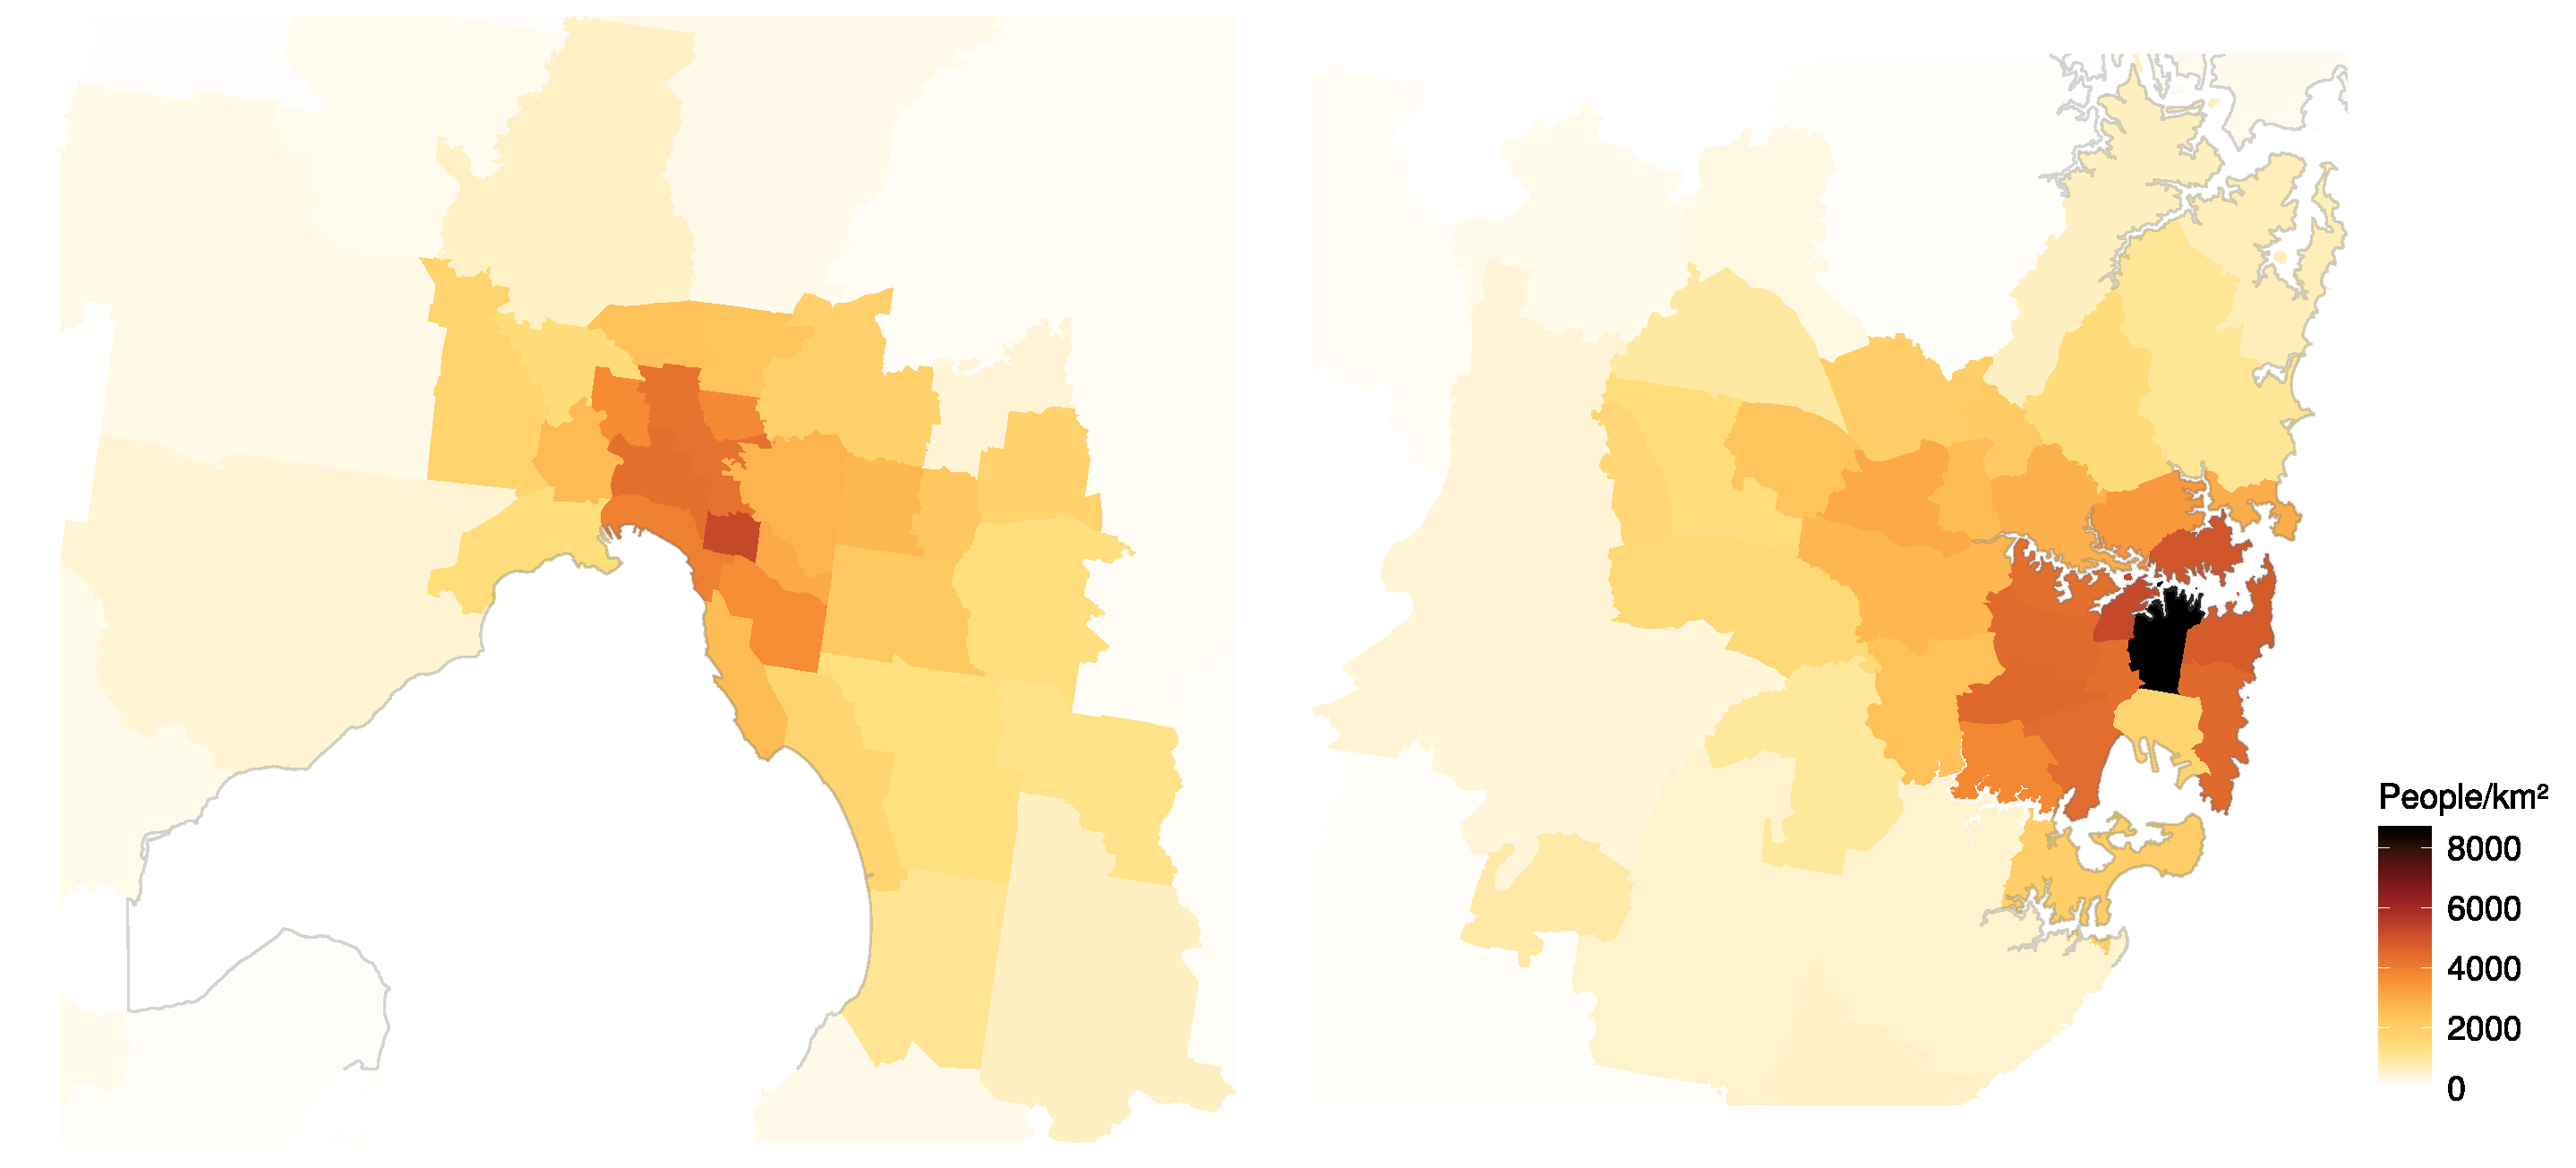
\includegraphics[width=2.164\columnwidth]{atlas/SYD_MEL_densities-1.pdf}
\noteswithsources{SA3 represent areas with populations between 30,000 and 130,000 persons and similar regional characteristics.}{\textcites{ABS-Census-2016}{R-Census2016.DataPack}.}
\end{figure*}

\begin{figure*}
\caption{\dots{} and Sydney has a much denser core of employment \label{fig:sydney-vs-melbourne-employment-density}}
\units{Density of jobs, 2011 Census, by SA3}
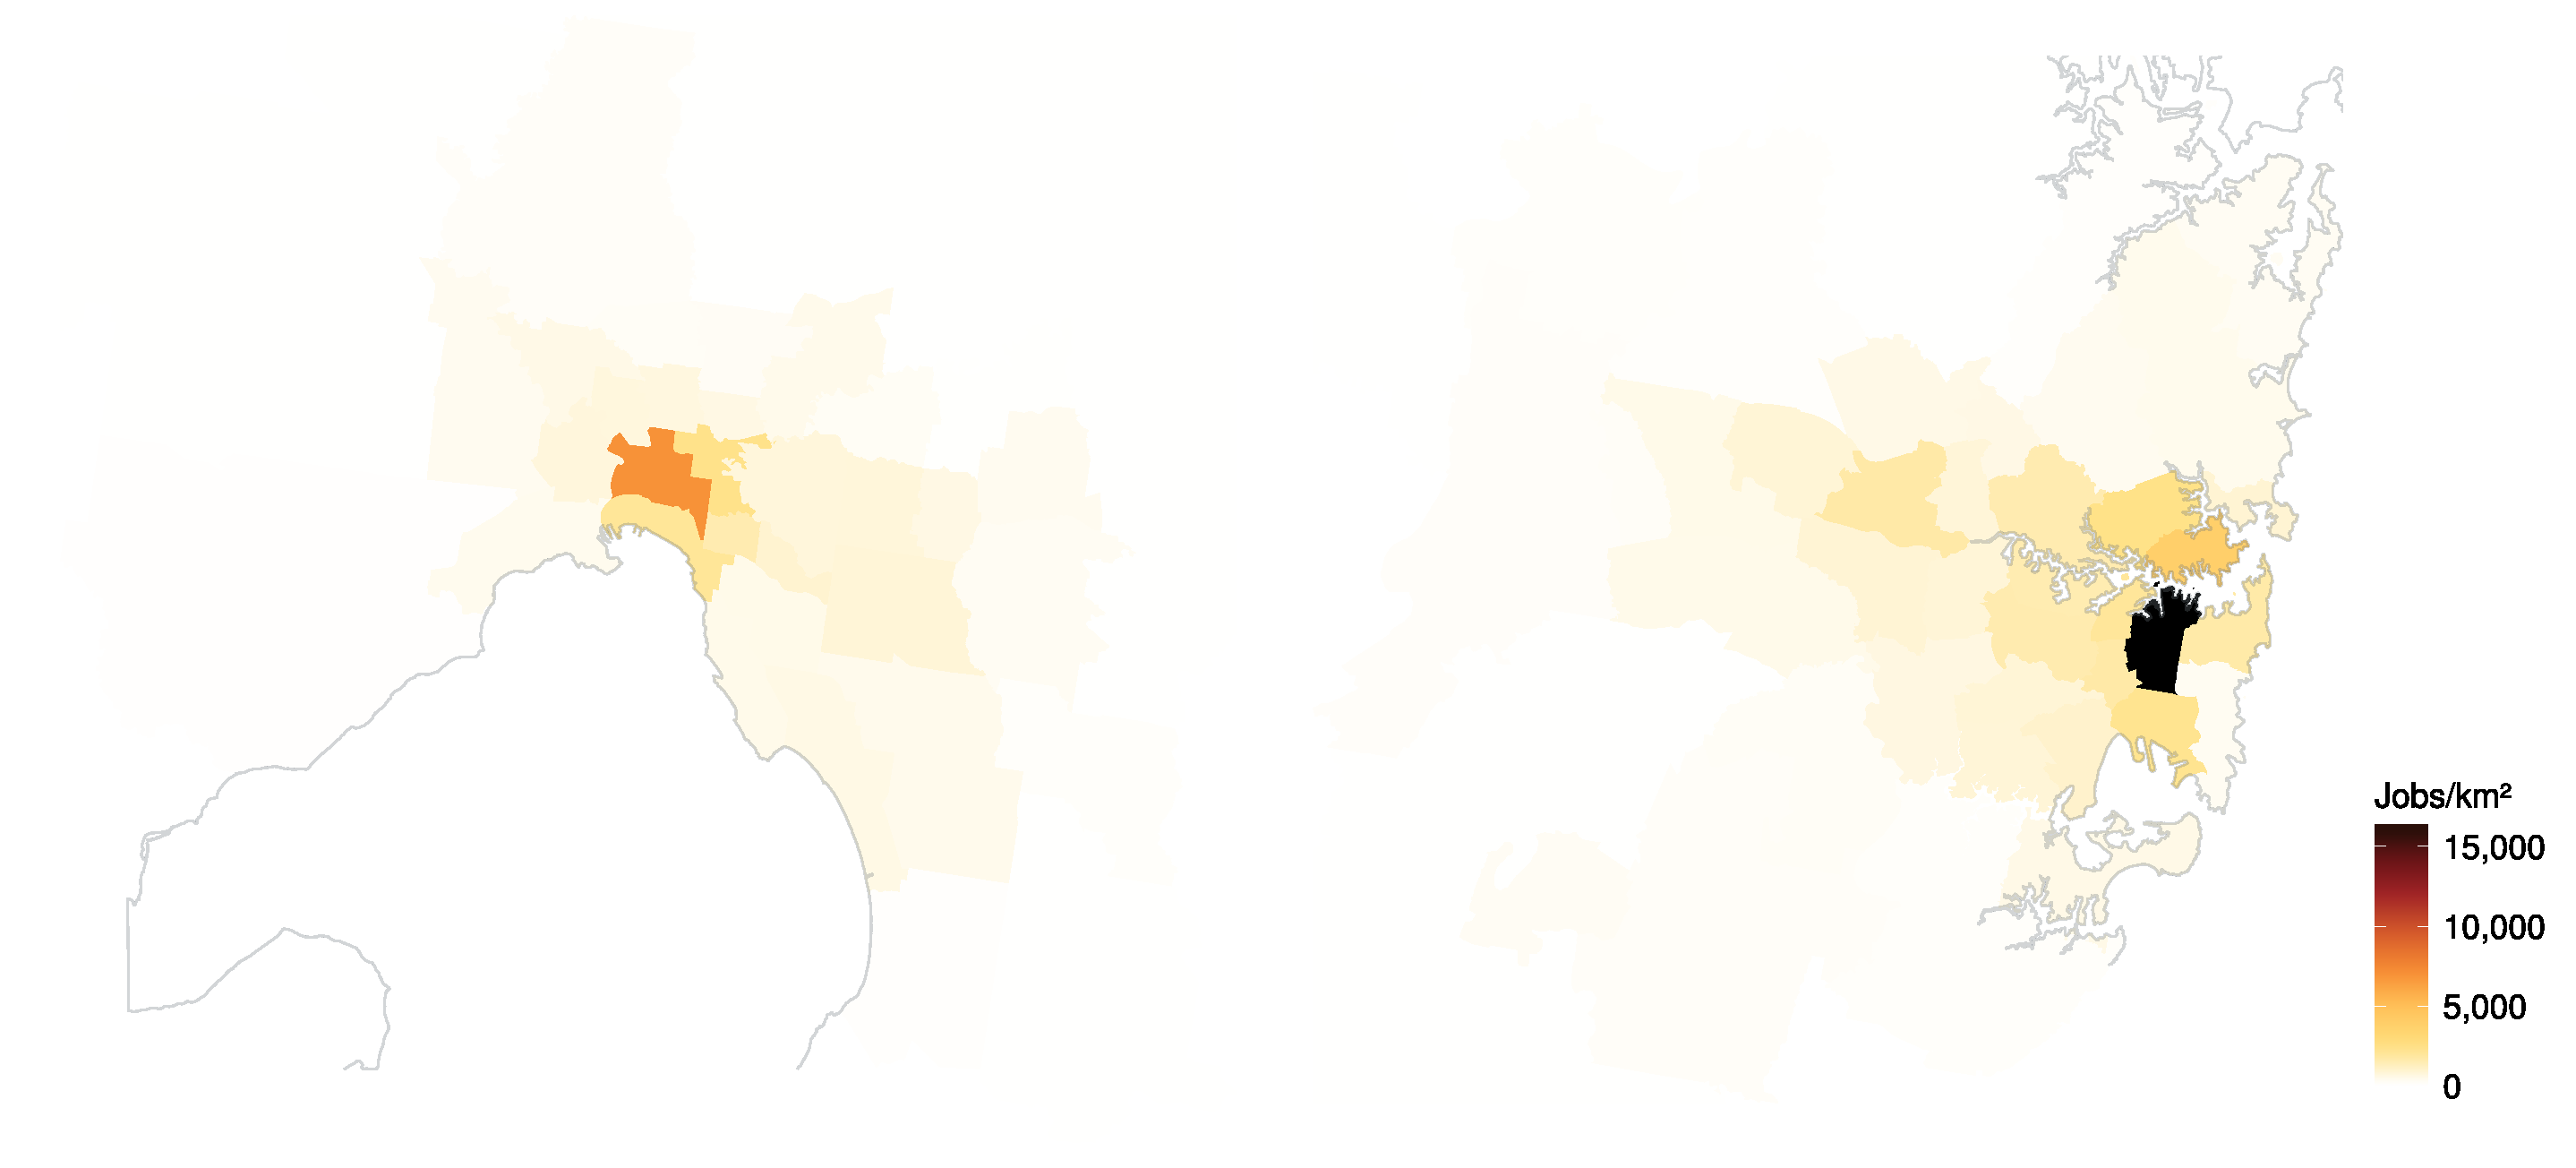
\includegraphics[width=2.164\columnwidth]{atlas/SYD_MEL_work_densities-1.pdf}
\noteswithsources{SA3 represent areas with populations between 30,000 and 130,000 persons and similar regional characteristics.}{\textcite{ABS2011Census}.}
\end{figure*}


\subsection{Sydney's topography is challenging}

Sydney is spread around a range of waterways; Port Jackson extends well into middle-ring suburbs.
As a result, many parts of the city rely on bridges -- which can form natural bottlenecks that create delays and reduce reliability.

Arguably Sydney's worst road congestion is between Balgowlah near Manly across The Spit, down through Mosman and Cremorne over the Harbour.
The Spit Bridge is unusual in that it opens regularly to allow yachts to navigate up Middle Harbour.
Mercifully, with 70,000 motorists using the Spit bridge daily, bridge openings are scheduled well outside peak periods, with the first opening at 10:15 every morning. \footcite{RMS-2017-bridge-opening-times}

Even with the bridge down, morning delays on this route are greater and less predictable than in the rest of Sydney (\Vref{fig:SpitReliability}).
Balgowlah commuters must allow 40 minutes to reliably get to work on time, 10~minutes longer than the normal morning commute, and 23~minutes, or 135~per cent, longer than the trip would take without traffic.%
    \footnote{Based on the duration in traffic for the 95th percentile.}

The commute from Drummoyne to the CBD tells a similar story.
With no traffic the trip, over the Iron Cove and Anzac bridges, takes about 10~minutes.
The morning commute typically takes more than 21~minutes, but the delay is highly variable: in a typical week the duration of the morning commute varies between 16 and 26 minutes.


\begin{figure}
  \caption{Trips across The Spit are much more delayed and unpredictable than trips in the rest of Sydney}\label{fig:SpitReliability}
  \units{Distribution of extra minutes relative to free flow, weekday commutes to employment centres between 6\,am and 10\,am}
  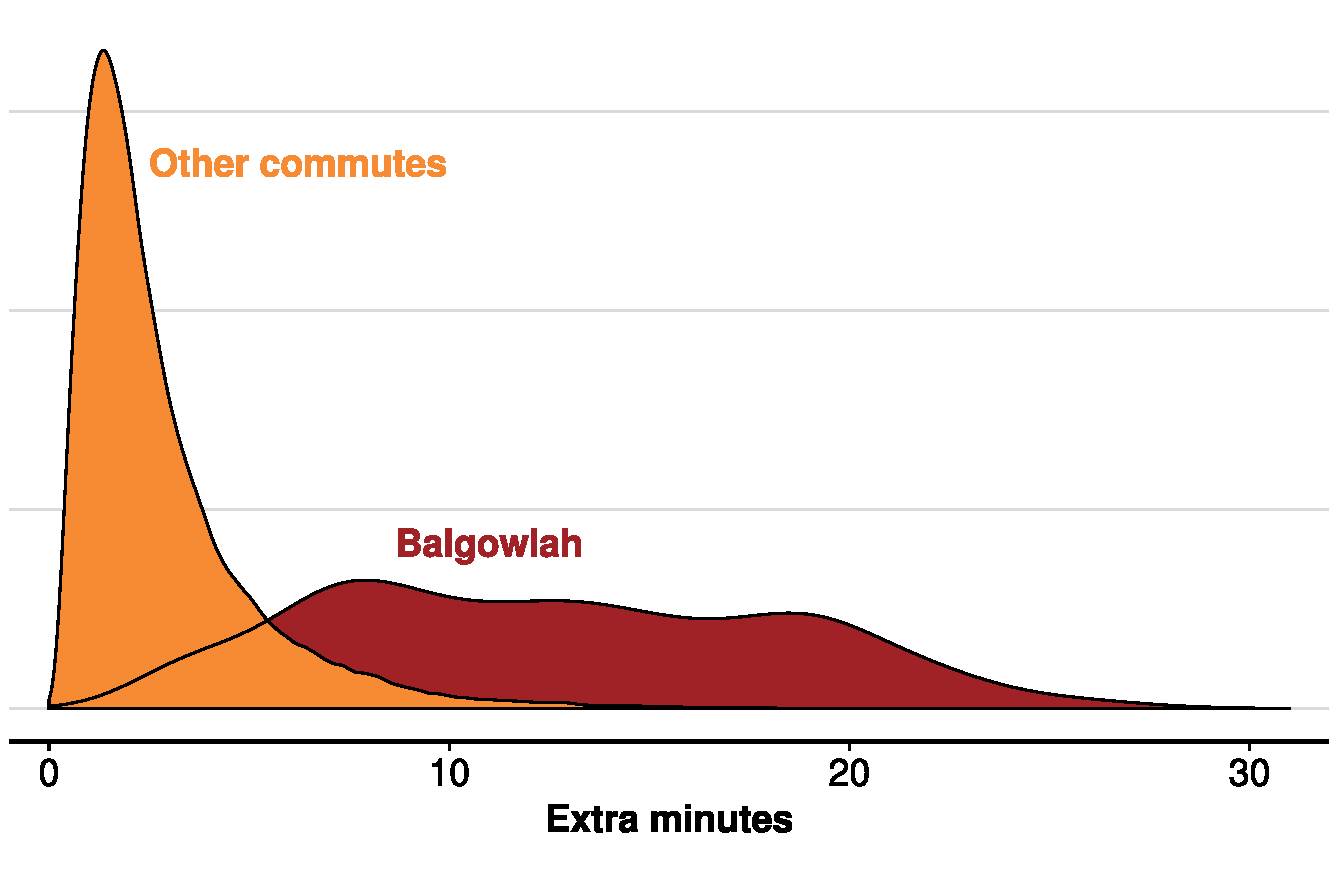
\includegraphics{atlas/density-Balgowlah-vs-other-SYD-commutes--MonFri6-10-1.pdf}
  \notes{Excludes public holidays.
Excludes commutes with fewer than 400~drivers.}
\end{figure}


\subsection{Congestion is worse in suburbs without rail}

\begin{figure*}
\caption{Suburbs without railways have more CBD commuters by car}\label{fig:above-below-average-n-drivers--InnerSydney}
\units{Number of commuters to Sydney's CBD by car}
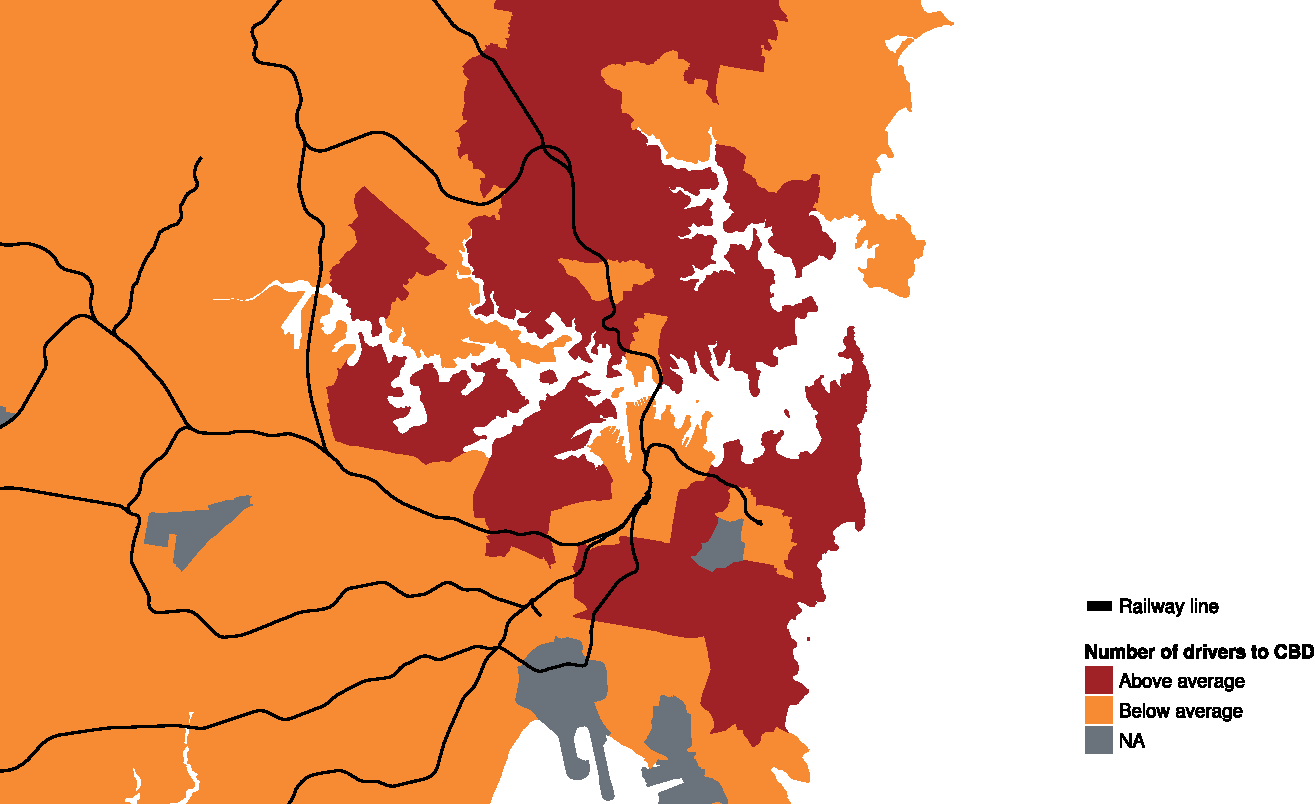
\includegraphics[width=1.9\columnwidth]{atlas/chloropleth-n-drivers--Sydney-CBD-1-crop.pdf}
\notewithsource{Average is over all SA2s visible.}%
{Grattan analysis of \textcite{ABS2011Census}}
\end{figure*}

Routes where commuters have access to rail tend to have less road congestion than those without rail.
For example, drivers from the North Shore to the CBD encounter less congestion than drivers from suburbs around Middle Harbour.
The North Shore is serviced by heavy rail; the Middle Harbour suburbs are not.

\begin{figure}
\caption{Congestion is worse in bridge-reliant suburbs without rail}\label{fig:railways-and-bridges-have-worst-congestion}
\units{Minutes of delay and increase travel time relative to free-flow, journeys to work, weekday morning peak, Sydney CBD}
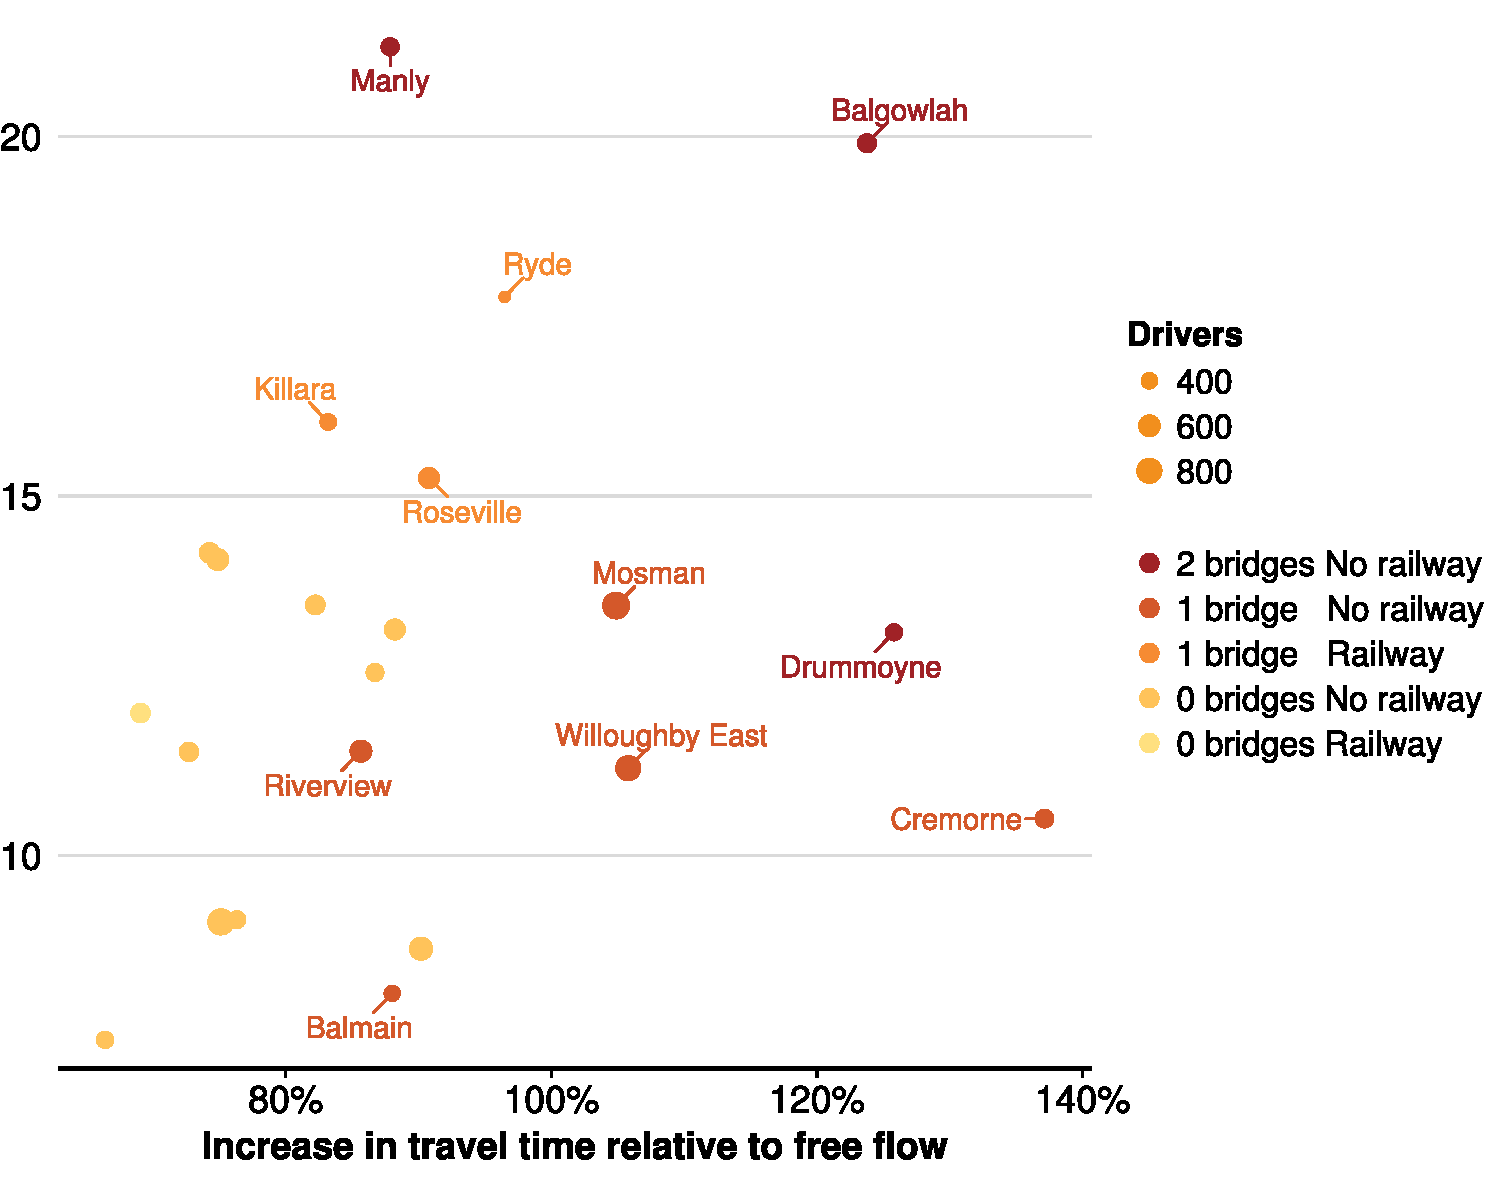
\includegraphics[width=1.125\columnwidth]{atlas/scatter-increase-in-travel-time-vs-free-flow-ratio--Sydney-1.pdf}
\notes{The size of each dot represents the number of drivers on the route.}
\end{figure}

Throughout inner and middle-ring Sydney, suburbs with a heavy rail line have fewer residents who drive to the CBD than suburbs without (see \Vref{fig:above-below-average-n-drivers--InnerSydney}).

Suburbs that have no rail line and are bridge-reliant have the worst road congestion of all, as shown in \Vref{fig:railways-and-bridges-have-worst-congestion}.

Use of Sydney's passenger rail network is growing rapidly.
In 2016-17, the number of passengers increased by more than 10 per cent.%
\footcite{TrNSW-2017-MonthlyTransportPatronage}

Such growth may ease road congestion, but it comes at a cost. Measured more than a year ago, almost all services arriving at Central between 8\,am and 9\,am on the T4 Eastern Suburbs and Illawarra Line were over-crowded by the time they reached Sydenham station.%
    \footnote{A load factor of 135 per cent of seated capacity is the benchmark beyond which passengers experience crowding and longer dwell times at stations can compromise punctuality. \textcite[][March~2016]{TrNSW-2017-TrainLoadsByLine}.}
Sydney's rail network clearly takes pressure off the roads, but it has limited reach and is under increasing capacity pressure.


\subsection{Sydney's toll roads have not been designed to manage congestion}

Sydney already has an extensive network of toll roadways,%
    \footnote{The Hills M2 Motorway, M4 and M5 East Freeway, M5 South-West Motorway, Westlink M7 Motorway, Eastern Distributor, Cross City Tunnel, Lane Cove Tunnel, Sydney Harbour Bridge, Sydney Harbour Tunnel, and the WestConnex New M4.}
and a host of new ones will   be added over the next decade.%
    \footnote{This includes the completion of NorthConnex and WestConnex stage two in 2019, and then WestConnex stage three, a Western Harbour Tunnel, a Beaches Link to the northern suburbs, and an extension of the F6 in the city's south.}
The cost of the toll per trip (comprising flagfall, per kilometre charge and toll cap) varies significantly across each of these roads.

Some argue that toll roads improve traffic flows in Sydney by enabling construction of new roads more quickly than would occur under more traditional funding models.%
    \footcite{BITRE-toll-roads-in-Australia}
But experience shows that introducing a toll on one part of the road network moves congestion to another part of the network.
The NSW Government's tolling principles emphasise revenue-raising but do not mention congestion-management.





\subsection{Some causes matter less -- weather and accidents}

So far this chapter has focused on normal recurrent congestion -- many  vehicles using the roads at the same time.
But congestion can also be caused by unusual events, such as severe weather or major incidents.
This section examines the impact of two major events in Sydney in the six months from March 2017: the wettest week of the period, and a particularly bad traffic incident.

\subsubsection{Heavy rain makes little difference to congestion}

We have not found evidence that rainfall contributes much to congestion.
On some rainy days, delays were longer, but on other rainy days, delays were shorter. There is some evidence that drivers on roads with poorer drainage or tighter corners may experience greater delays, but on the whole the effects are not particularly compelling.

This perhaps surprising finding is supported by other recent congestion research in Australia.%
    \footcites{Austroads-2016-Congestion-Reliability-Review}{Qld-TMR-2016-Understanding-causes-of-congestion}

\begin{figure*}
\caption{Sydney's wettest week in six months did not have unusual congestion}\label{fig:sydney-commutes-early-june-rain}
\units{Trip time, minutes for the Liverpool--CBD corridor, with morning and afternoon rainfalls}
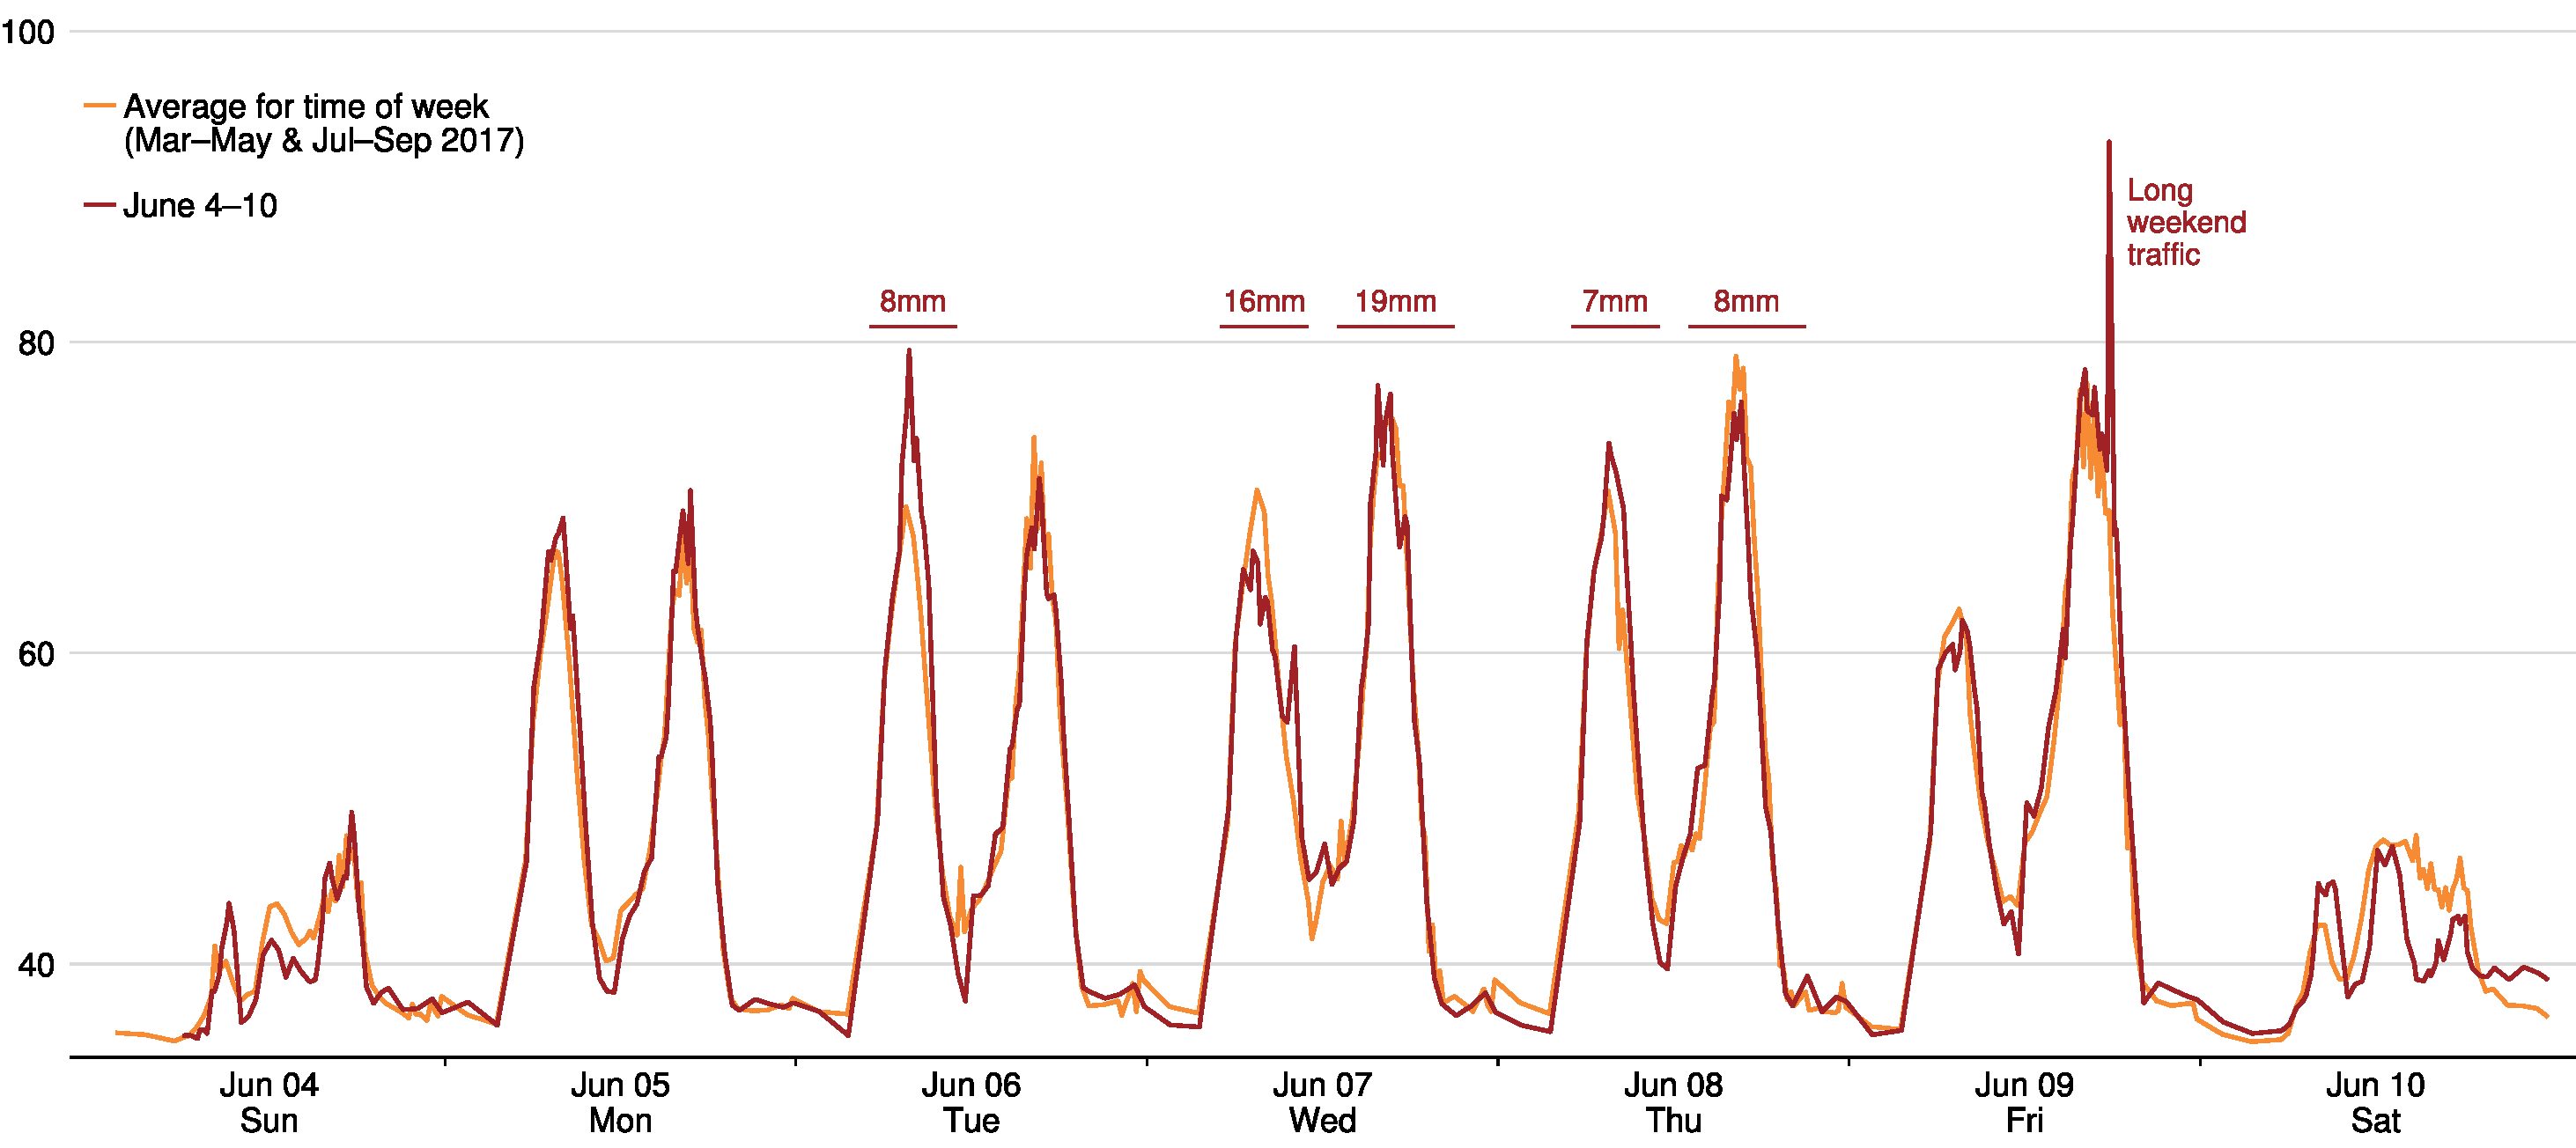
\includegraphics[width=\textwidth]{atlas/Liverpool-June-week-1.pdf}
\noteswithsources{Annotations in mm represent total precipitation between 5\,am and noon or between noon and 10\,pm at Sydney Airport.
Trip time is into the CBD in the morning and from the CBD after noon}%
{Grattan analysis of Google Maps data and \textcite{Bom-Data}.}
\end{figure*}

%\begin{figure*}
%\caption{Sydney's wettest week in six months did not have unusual congestion}\label{fig:sydney-commutes-coogee-early-june-rain}
%\units{Trip time, minutes for the Coogee--CBD corridor, with morning and afternoon rainfalls}
%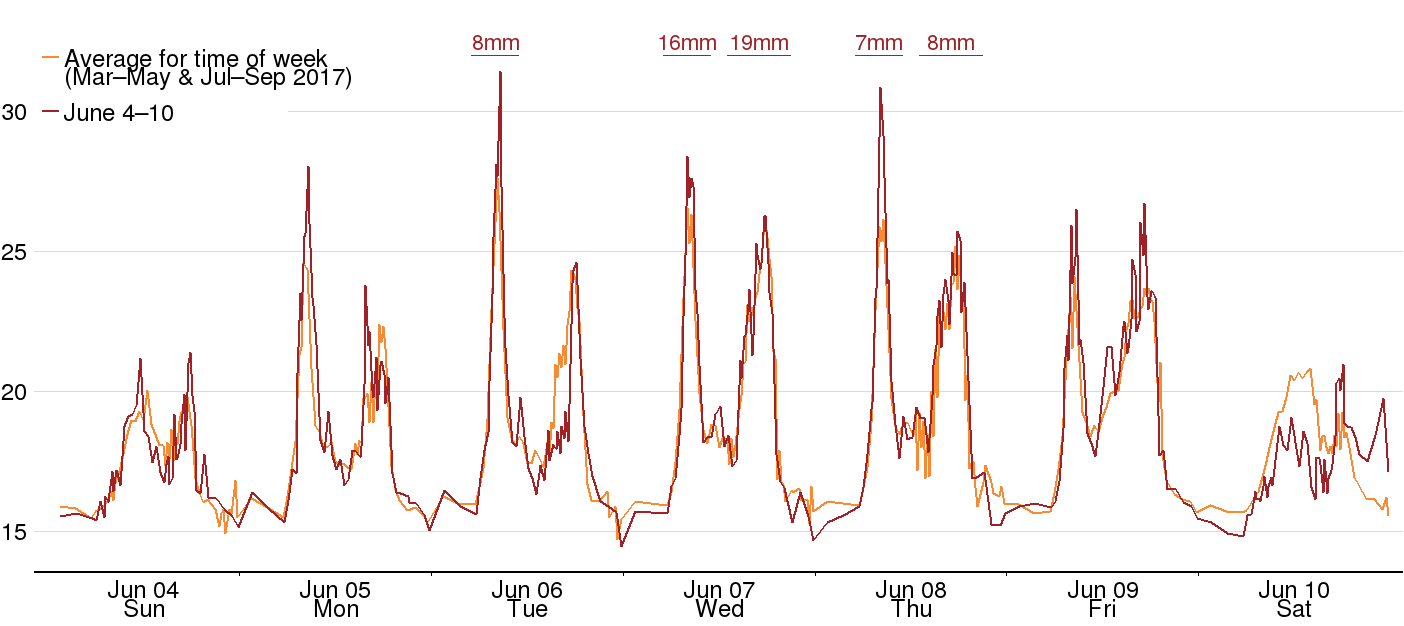
\includegraphics[width=\textwidth]{atlas/Coogee-June-week-1.pdf}
%\noteswithsources{Annotations in mm represent total precipitation between 5\,am and noon or between noon and 10\,pm at Sydney Airport.
%Trip time is into the CBD in the morning and from the CBD after noon}%
%{Grattan analysis of Google Maps data and \textcite{Bom-Data}.}
%\end{figure*}

The unremarkable difference between wet and dry days is best illustrated by the change in delays on the week leading up to the June long weekend. During this week Sydney experienced some of the heaviest rainfall of the sample period, with significant rainfall on Tuesday morning; all day Wednesday and Thursday; and Friday afternoon.
\footcite{Bom-Data}

Even during this week of heavy rainfall there was very little impact on average travel times across our sample. \Vref{fig:sydney-commutes-early-june-rain} shows the route between Liverpool and the CBD, which passes by the airport weather station. It shows that even when large amounts of rain were recorded there was very little change in travel times. In fact, during one of the biggest downpours on Wednesday morning the travel times were actually noticeably better than the average.

Similar results were found on other rainy days in Sydney.  In Melbourne, too, rain made little difference to congestion.%
    \footnote{For example, in Melbourne there was 2.8\,mm of rain on Wednesday 26 April, 6.6\,mm on Thursday 27 April, and no rain on Friday 28 April %
    (\textcite{Bom-Data}),
    yet congestion levels were the same across all three days.}

\subsubsection{Major incidents and accidents can be very disruptive}

Generalising about major incidents and accidents is difficult because each is unique.
But an examination of one of the worst incidents in Sydney in the six months from March 2017 illustrates that impacts on travel times can be positive as well as negative.



A power blackout in Arncliffe, just west of Sydney Airport, around 4\,pm on Friday 26 May 2017 knocked out 100 sets of traffic lights.%
  \footcite{ABC-2017-Arncliffe-blackout}
A 7\,km stretch of the M5 between the airport and Bexley North had to be closed and was not reopened until after 7\,pm.

The incident is clearly visible in our data, which contains 24~routes that pass through that section of the M5.
The severity of the congestion depended on the direction drivers were going: the trip from Enfield to the airport was 40 per cent longer than normal for that time of day
but in the other direction the delay was only 6 per cent.
And for people heading west from the airport, trip times were actually shorter than usual; with outbound traffic from the CBD unable to get through, drivers leaving the airport were spared much of the normal traffic.







\chapter{Where and why is congestion a problem in Melbourne?}\label{chap:Melbourne-congestion}

In Melbourne as in Sydney, most roads at most times are not in gridlock. But Melbourne is on track to become Australia's biggest city,%
    \footcite[][27]{IA-2015-State-of-Australian-Cities-2014-2015}
and congestion is rightly coming to be seen as a major problem.

The first part of this chapter shows that, during peak times, delays on trips to and from the CBD and its surrounding suburbs and on trips between the city and north-eastern suburbs are reaching concerning levels.

The second part of the chapter identifies three key causes: the way Melbourne's CBD dominates the city's economy, the relative attractiveness of driving in the CBD and surrounds, and the design of Melbourne's toll road pricing.

\section{Melbourne's CBD and surrounds are very congested}

On the face of it, Melbourne's congestion is similar to Sydney's. Both cities have congested roads during the morning and afternoon peaks, and trip times 65 per cent longer than free-flow conditions are normal (\Vref{fig:Melb-CBD-v-Non-CBD-commutes}).

\begin{figure}
\captionsetup{oneside,margin={0em,-1em}}
\caption{Melbourne's CBD commuters face higher delays than Sydney's}\label{fig:Melb-CBD-v-Non-CBD-commutes}
\units{Increase in travel time relative to free-flow}
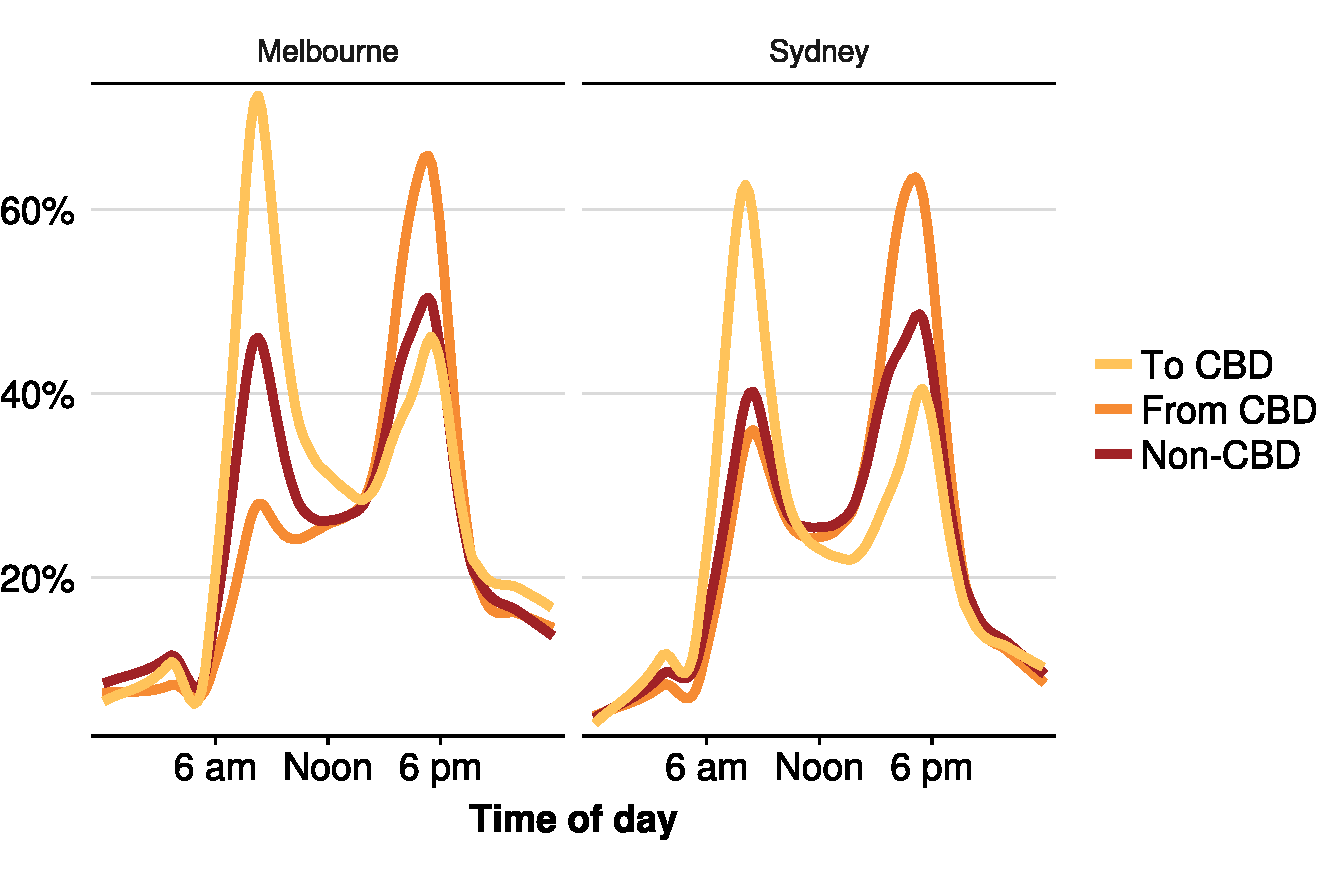
\includegraphics{atlas/increase-in-travel-time-vs-time-of-day-by-Classification-CBD-commuting--facet-by-City-1.pdf}
\noteswithsource{Based on travel time of representative route samples collected via Google Maps.
For details of routes see Appendix.
Weekends and public holidays excluded}{Grattan analysis based on data from Google Maps}
\end{figure}

Trips to Melbourne's CBD from the suburbs in our sample take, on average, around 25 minutes when there is no traffic.%
    \footnote{See \Chapref{chap:Routes-sampled} for details of the CBD commuting trips included in the sample.}
These trips are delayed by around 18 minutes (or close to 80~per cent) during the morning peak, compared to the time they would take in the middle of the night. Trips are not as delayed in the afternoon peak, at around 13 minutes (or over 60 per cent) longer due to traffic -- but the afternoon peak lasts longer and is therefore harder to avoid.

Average delays are much shorter for people driving to other employment centres such as Clayton, Dandenong, Box Hill or the La Trobe University precinct than to the CBD\@.
Morning delays peak at around 11 minutes, or 58 per cent, for a trip that would take 21 minutes in free-flow conditions. 

While most motorists in outer areas experience low levels of congestion, isolated pockets of congestion -- ``hotspots'' -- do exist. For example, we see evidence of bottlenecks in Melbourne's outer south-eastern suburbs, consistent with the \citeauthor{Redspotsurvey}'s \citetitle{Redspotsurvey} findings.%
    \footnote{\citeauthor{Redspotsurvey} \citetitle{Redspotsurvey} found bottlenecks in middle and outer suburbs, including the Thompsons Road / Western Port Highway roundabout in Skye (south-eastern Melbourne) and Point Cook Road between Sneydes Road and Princes Freeway in Seabrook (south-western Melbourne).}

Although Melbourne and Sydney have similar average delays, commuters to Melbourne’s CBD are typically be more delayed than those to Sydney’s CBD\@. And these delays affect not only people commuting to work in the city, but also people travelling to work in other places, drivers of trucks and vans, tradespeople, students and shoppers.

These delays can be isolated to the congestion on key arterial roads in inner Melbourne. Drivers using Hoddle Street, Punt Road, Church Street, Victoria Parade and Princes Street can expect delays significantly above the average for CBD commutes in general (see \Vref{fig:HoddleStreet-vs-time_of_day}).

\begin{figure}
\caption{Arterial roads in suburbs immediately surrounding Melbourne's CBD are particularly delayed}\label{fig:HoddleStreet-vs-time_of_day}
\units{Increase in travel time relative to free flow}
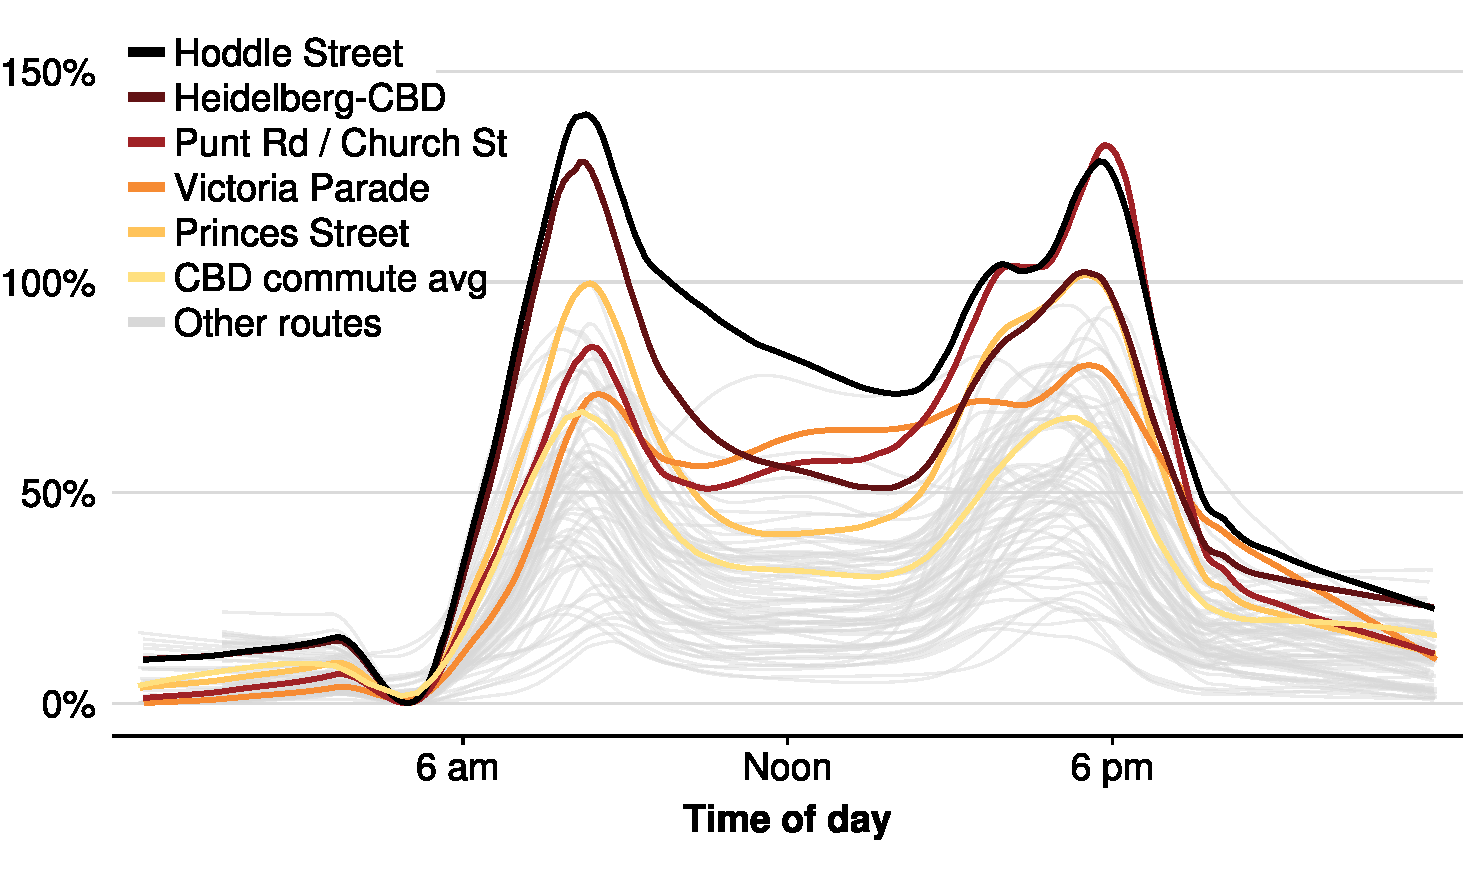
\includegraphics[width=1.1\columnwidth]{atlas/HoddleStreet-vs-others-1.pdf}
\noteswithsource{Average delay is calculated as the ratio of trip duration at each point throughout the day to the minimum trip duration observed for that route over the sample period. Based on travel time of representative route samples collected via Google Maps available in \Chapref{chap:Routes-sampled}.
Weekends and public holidays excluded}{Grattan analysis based on data from Google Maps}
\end{figure}

\Vref{fig:HoddleStreet-vs-time_of_day} also points to another characteristic of congestion in Melbourne: unlike Sydney, there is a one specific geographic compass point where travel to and from the CBD is significantly more congested -- the north east, such as Heidelberg.
The following two sections explain the lower reliability and higher delays for people travelling to or from this part of the city.










%
%peak_summary_by_ROUTE_ID_Date_AMPM %>% City_by_ROUTE_ID[., on = "ROUTE_ID"] %>% Classification_by_ROUTE_ID[., on = "ROUTE_ID"] %>% .[City == "Melbourne"] %>% .[Classification == "CBD commuting - to city"] %>% .[, Wkday := weekdays(Date)] %>% .[Wkday %notin% c("Saturday", "Sunday")] %>% .[AM == "AM"] %>% free_flow_by_ROUTE_ID[., on = "ROUTE_ID"] %>% .[Date %notin% public_holiday_dates[["Date"]]] %$% mean(peak_duration / free_flow)

%
%
% peak_summary_by_ROUTE_ID_Date_AMPM %>% City_by_ROUTE_ID[., on = "ROUTE_ID"] %>% Classification_by_ROUTE_ID[., on = "ROUTE_ID"] %>% .[City == "Melbourne"] %>% .[Classification == "CBD commuting - to city"] %>% .[, Wkday := weekdays(Date)] %>% .[Wkday %notin% c("Saturday", "Sunday")] %>% .[AM == "PM"] %>% free_flow_by_ROUTE_ID[., on = "ROUTE_ID"] %>% .[Date %notin% public_holiday_dates[["Date"]]] %$% mean(peak_duration / free_flow)



\begin{figure*}
\caption{Melbourne's worst congestion is in the north east}\label{fig:MEL-map-P50-80-90}
\units{CBD commutes, ratio quantiles measured over weekday trips between 7\,am and 9:30\,am}
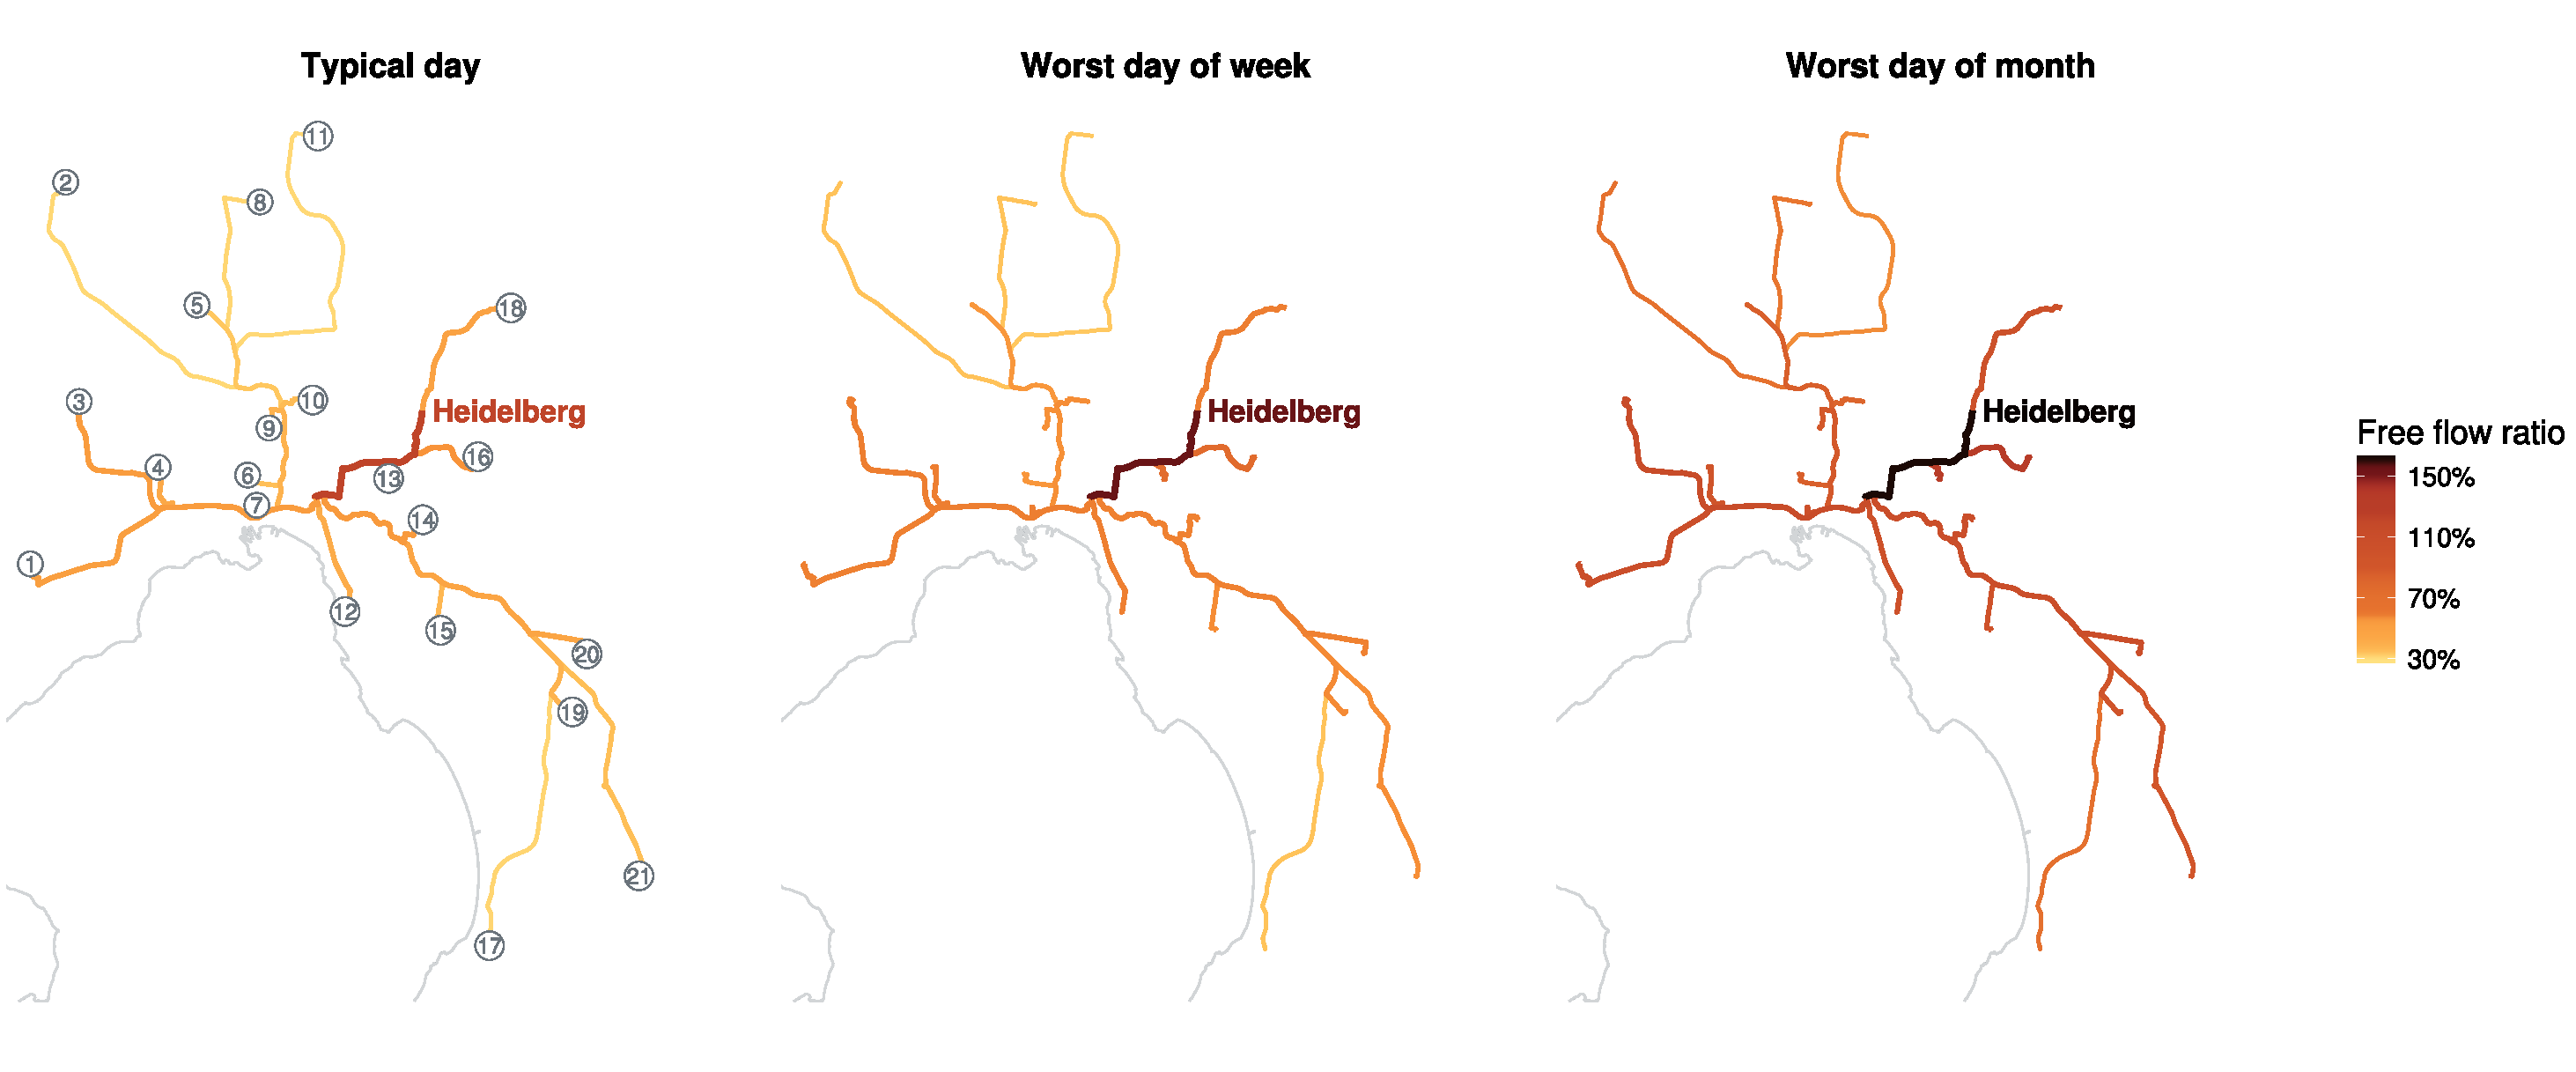
\includegraphics[width=\textwidth]{atlas/plot_three_MEL-1}
\newcolumntype{z}{>{\footnotesize\arraybackslash}r}
\newcolumntype{y}{>{\footnotesize\arraybackslash}X}
\addtolength{\tabcolsep}{-2pt}
% \begin{tabularx}{0.95\textwidth}{zyzyzyzyzyzyzyzy}
% 1. & Hoppers Crossing & 2. & Sunbury        & 3. & Caroline Springs & 4. & Sunshine West & 5.  & Melbourne Airport & 6. & Footscray        & 7. & Port Melbourne \\
% 8. & Craigieburn      & 9. & Moonee Ponds  & 10. & Coburg &
% 11. & Donnybrook & 12. & Brighton & 13. & Kew & 14. & Camberwell \\
% 15. & Oakleigh South & 16. & Doncaster & 17. & Frankston & 18. & Diamond Creek & 19. & Dandenong & 20. & Rowville & 21. & Cranbourne \\
% \end{tabularx}
% latex table generated in R 3.4.1 by xtable 1.8-2 package
% Mon Oct 02 02:25:09 2017
\begin{tabularx}{0.43\textwidth}{zyzyzy}
  1. & Hoppers Crossing & \phantom{.} 8. & Craigieburn & \phantom{.} 15. & Oakleigh South \\ 
  2. & Sunbury & \phantom{.} 9. & Moonee Ponds & \phantom{.} 16. & Doncaster \\ 
  3. & Caroline Springs & \phantom{.} 10. & Coburg & \phantom{.} 17. & Frankston \\ 
  4. & Sunshine West & \phantom{.} 11. & Donnybrook & \phantom{.} 18. & Diamond Creek \\ 
  5. & Melbourne Airport & \phantom{.} 12. & Brighton & \phantom{.} 19. & Dandenong \\ 
  6. & Footscray & \phantom{.} 13. & Kew & \phantom{.} 20. & Rowville \\ 
  7. & Port Melbourne & \phantom{.} 14. & Camberwell & \phantom{.} 21. & Cranbourne \\ 
  \end{tabularx}

\end{figure*}

\subsection{Trips to and from the north east are less reliable}

People travelling from Melbourne's north-eastern suburbs to the city tend to experience the highest delays.
And the extent of the delays is hard to predict.

\Vref{fig:MEL-map-P50-80-90} shows the delays motorists travelling between a range of locations and the CBD would face on a typical day, on the worst day in a week, and on the worst day in a month.

The greatest delays are from the north-eastern suburbs of Heidelberg, Doncaster and Kew.
The first panel shows travel from Heidelberg during the morning peak on a typical day takes twice as long as it would with no traffic.
By contrast, motorists coming from other parts of Melbourne, such as Sunbury in the north-west, Craigieburn and Donnybrook in the north, and Frankston in the south-east, face delays of less than 40 per cent on a typical weekday morning.%
    \footnote{The delay relative to free flow tends to reduce with distance.
This is because drivers coming from the outer suburbs spend only part, rather than all, of their trip in the high concentration of traffic.}

The second panel shows the congestion commuters typically face on the worst morning in a week.
Most routes can expect one day a week when trip times takes 70 per cent longer than it would with no traffic.
Travellers from Doncaster, Kew, and Heidelberg who travel in the morning peak can expect their commute to take twice as long as it does without traffic.

The third panel shows the delays a commuter would face on the worst day in a month.
When traffic is this bad, the morning commute from Heidelberg takes more than two-and-a-half times as long in the peak as it does in free-flow conditions.
Most motorists travelling from the west, east, and south-east spend more than double the free-flow travel times in traffic once a month.

% peak_summary_by_ROUTE_ID_Date_AMPM %>%
%   Suburbs_by_ROUTE_ID[., on = "ROUTE_ID"] %>%
%   .[orig_Suburb == "Doncaster" & dest_Suburb == "CBD"] %>%
%   .[, Weekday := weekdays(Date)] %>%
%   .[Weekday %notin% c("Saturday", "Sunday")] %>%
%   .[AM == "AM"] %>%
%   .[Date %notin% public_holiday_dates[["Date"]]] %$%
%   quantile(peak_duration, probs = c(0.2, 0.8, 0.95))

%        20%      80%      95%
% 28.80333 44.04667 47.70500
This variability in travel time makes it difficult for motorists to plan their travel because people need a buffer for each trip they make. For example, a trip from Doncaster to the city with no traffic takes around 20 minutes, and during the morning peak it takes twice as long, on average.
But a commuter who does this commute regularly also knows that in any given week, on one day it may take 29 minutes, and another day 44 minutes. And once a month it takes 48 minutes, about 20 minutes longer than it takes once a week.


\doublecolumnfigure{
\captionsetup{oneside,margin={0em,-0.8em}}
 \caption{\label{fig:NSEW_Melb}Travel delays are most acute for commuters from the north east}
\units{Increase in travel time relative to free flow, CBD commutes}
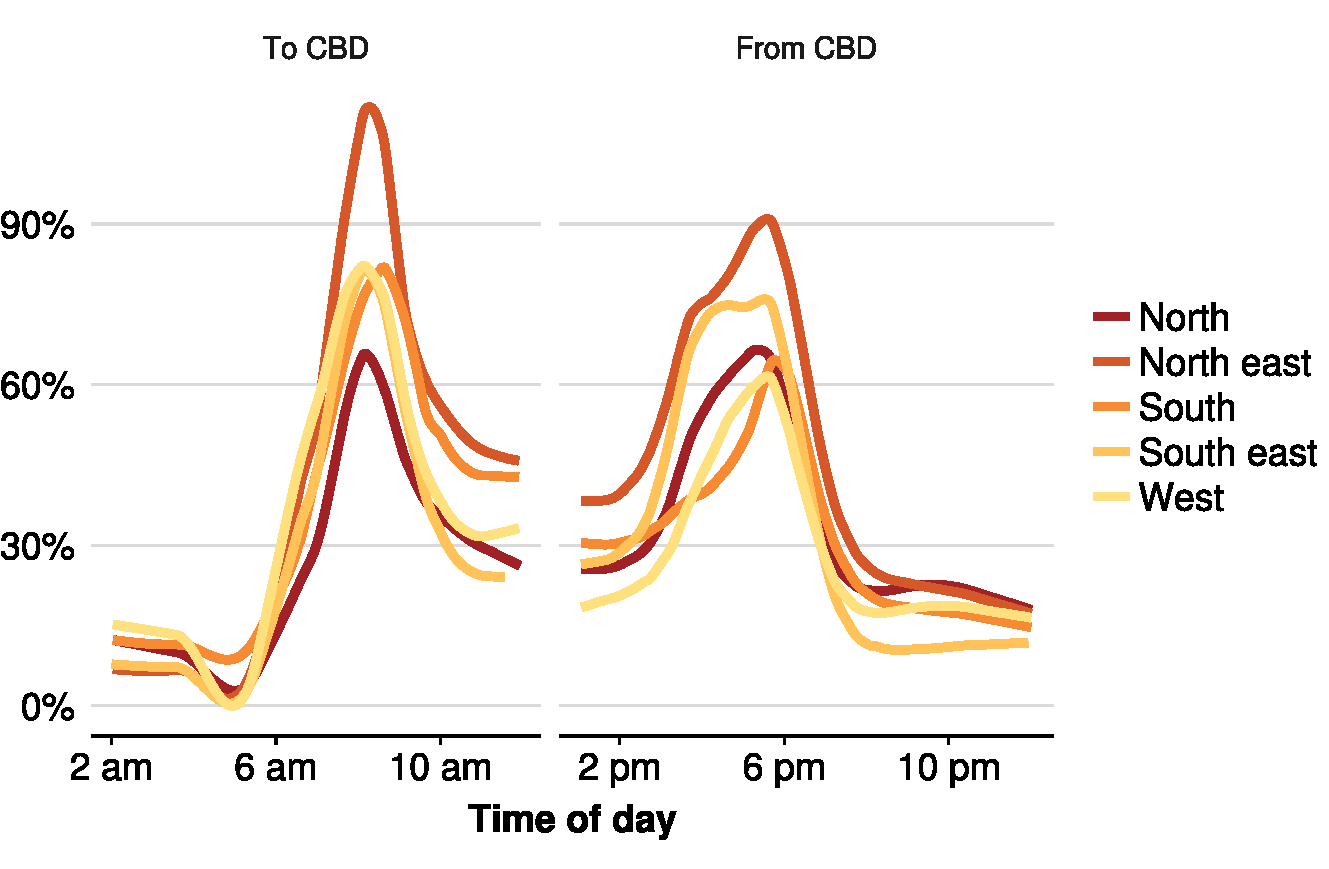
\includegraphics{atlas/Increase-in-travel-time-vs-hour-of-day-by-Location-Melbourne-MonFri-excl-holiday-1.pdf}
\noteswithsource{Average delay is calculated as the ratio of trip duration at each point throughout the day to the minimum trip duration observed for that route over the sample period. Routes to the north east include: Heidelberg, Doncaster, Kew and Diamond Creek.
Routes to the south east include: Dandenong, Cranbourne, Rowville, Oakleigh and Camberwell.
Routes to the south include: Port Melbourne, Brighton and Frankston.
Routes to the west include: Footscray; Hoppers Crossing, Sunshine West and Caroline Springs.
Routes to the north include: Coburg, Moonee Ponds, Melbourne Airport, Sunbury, Donnybrook and Craigieburn.
Weekends and public holidays excluded}{Grattan analysis based on data from Google Maps}
}{
\caption{CBD commutes from the north east are less reliable}\label{fig:boxplot_NE_highlight}
\units{Increase in travel time as a proportion of free flow, weekday morning peak, commutes into Melbourne CBD}
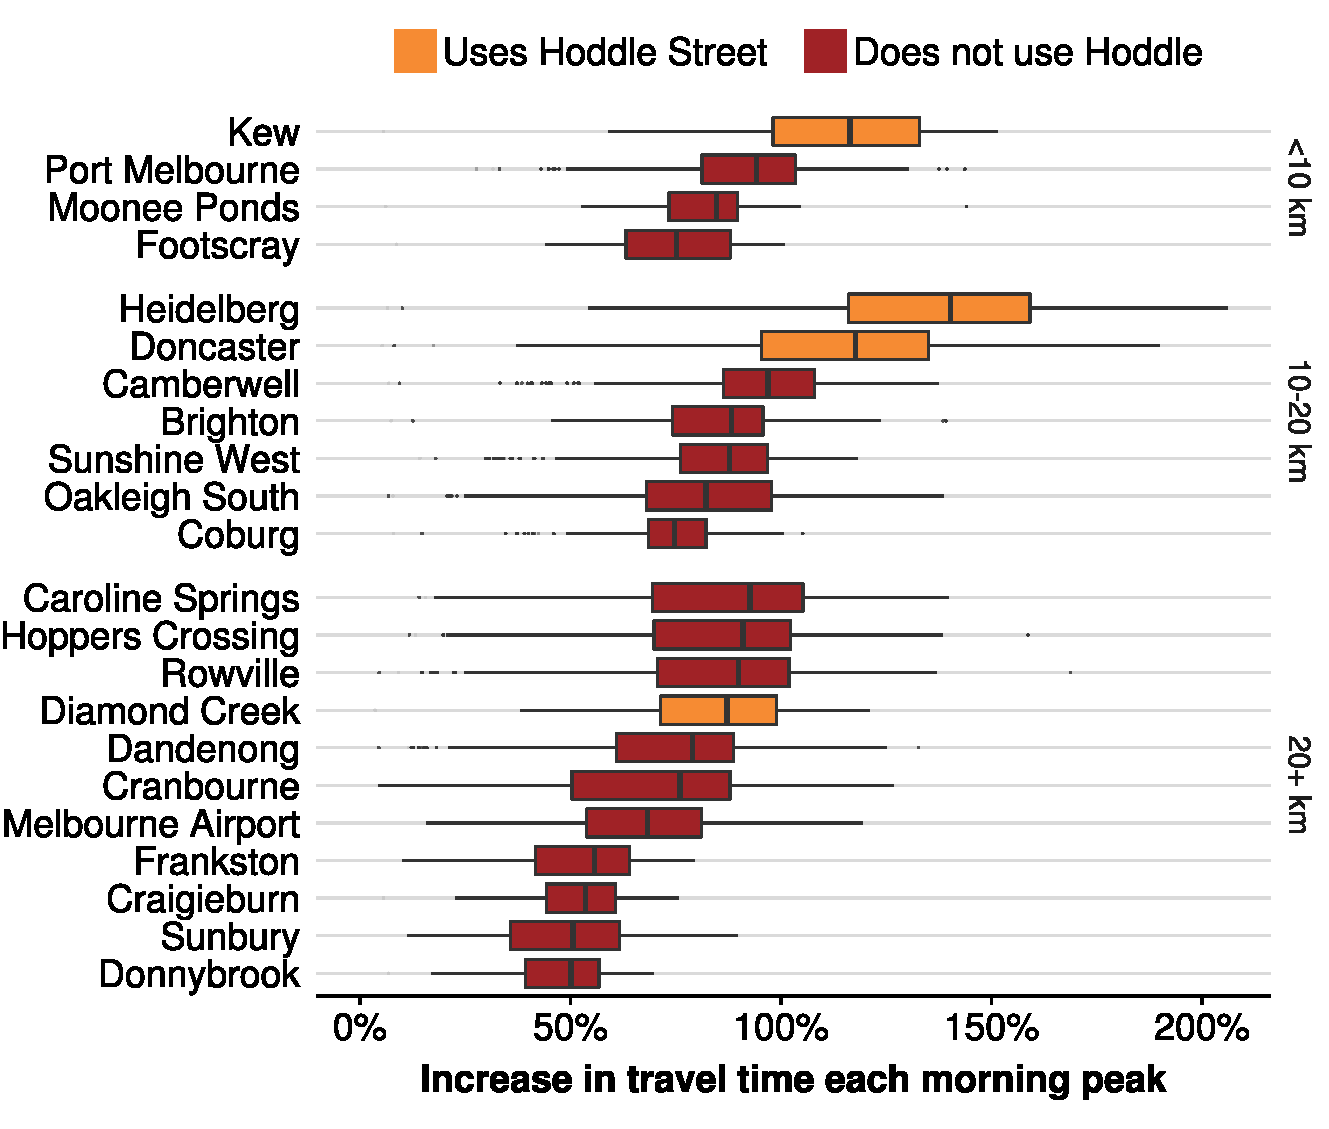
\includegraphics{atlas/boxplot-increase_in_travel_time-by-PuntRdness-facet-distance--CBD-commutes-to-cityr-1.pdf}
\noteswithsource{For travel departing between 7\,am and 9\,am.
Excludes weekends and public holidays. The boxes cover the 25th to 75th percentiles. The vertical line in each box lies at the median for each city. The `whiskers' on each side of the boxes extend no further than \(\pm1.5w\) where \(w\) is the box width. Observations beyond the lines are plotted as dots.}%
{Grattan analysis based on data from Google Maps.}
}

\subsection{The Eastern Freeway and Hoddle Street are a big part of the problem}

\Cref{fig:MEL-map-P50-80-90} shows that congestion is worst on routes coming into the city from the north-eastern suburbs.
The average delays for CBD travellers from the north-east in the morning peak are almost 120 per cent, whereas they are around 70 per cent for commuters from other directions (see \Vref{fig:NSEW_Melb}).



But we can be more precise about the locus of the problem. Commuters from the north-eastern suburbs typically drive in on the Eastern Freeway and Hoddle Street, a major north-south arterial. Hoddle Street trips in peak periods are routinely delayed by 130 per cent relative to free-flow travel times.%
    \footnote{130 per cent is the average weekday peak delay between Prahran Market and Clifton Hill railway station.}

The Eastern Freeway--Hoddle Street corridor has not only some of Melbourne's worst delays, but also some of the city's least reliable travel times. Motorists from suburbs to the north east (except Diamond Creek) face less reliable travel times than people travelling similar distances from other directions (\Vref{fig:boxplot_NE_highlight}).%
    \footnote{Diamond Creek has more reliable travel times than other suburbs in the north-east because it has an alternative route to the city via the Western Ring Road and Tullamarine Freeway.
Google Maps regularly selects this route because of long delays on the more direct Eastern Freeway -- Hoddle Street route.}

\section{Melbourne's congestion has several causes}%\label{section:no-single-cause}

The next sections of this chapter examine three main causes of Melbourne's congestion problem: the dominance of the CBD, the attractiveness of parking in the city, and the pricing structure of the city's toll roads.
The chapter ends with a look at the effects of unusual occurrences such as rain and accidents.

\subsection{Melbourne's CBD focal point is a factor}

We saw in \Vref{fig:aggregate-delay-CBD-commutes} that travel delays to and from Melbourne’s CBD are marginally worse than for similar trips in Sydney.
As in Sydney, these delays arise because the CBD is such an important focal point of the city's economic activity.

But in Sydney, the economic centre of gravity is drifting steadily towards the west, whereas in Melbourne, the CBD is intensifying as the city's economic powerhouse.%
\footcite{2016-Rasmussen-changing-business-location}
According to the 2011 Census, each day around 150,000 workers commute into central Melbourne, and 
almost one-third of them travel by car, twice the share in Sydney.%
	\footnote{This does not include those who commute to Southbank and Docklands precincts which also have a substantial number of jobs: \textcite{ABS2011Census}.}
It is therefore not surprising that delays on travel to and from the CBD are longer than those in Sydney.


\subsection{Driving remains attractive in Melbourne, even in the CBD}

\begin{figure}[t]
\caption{More and more people are driving into Melbourne's CBD\label{fig:drivers-to-Melb}}
\units{Change in number of workers driving to the CBD}
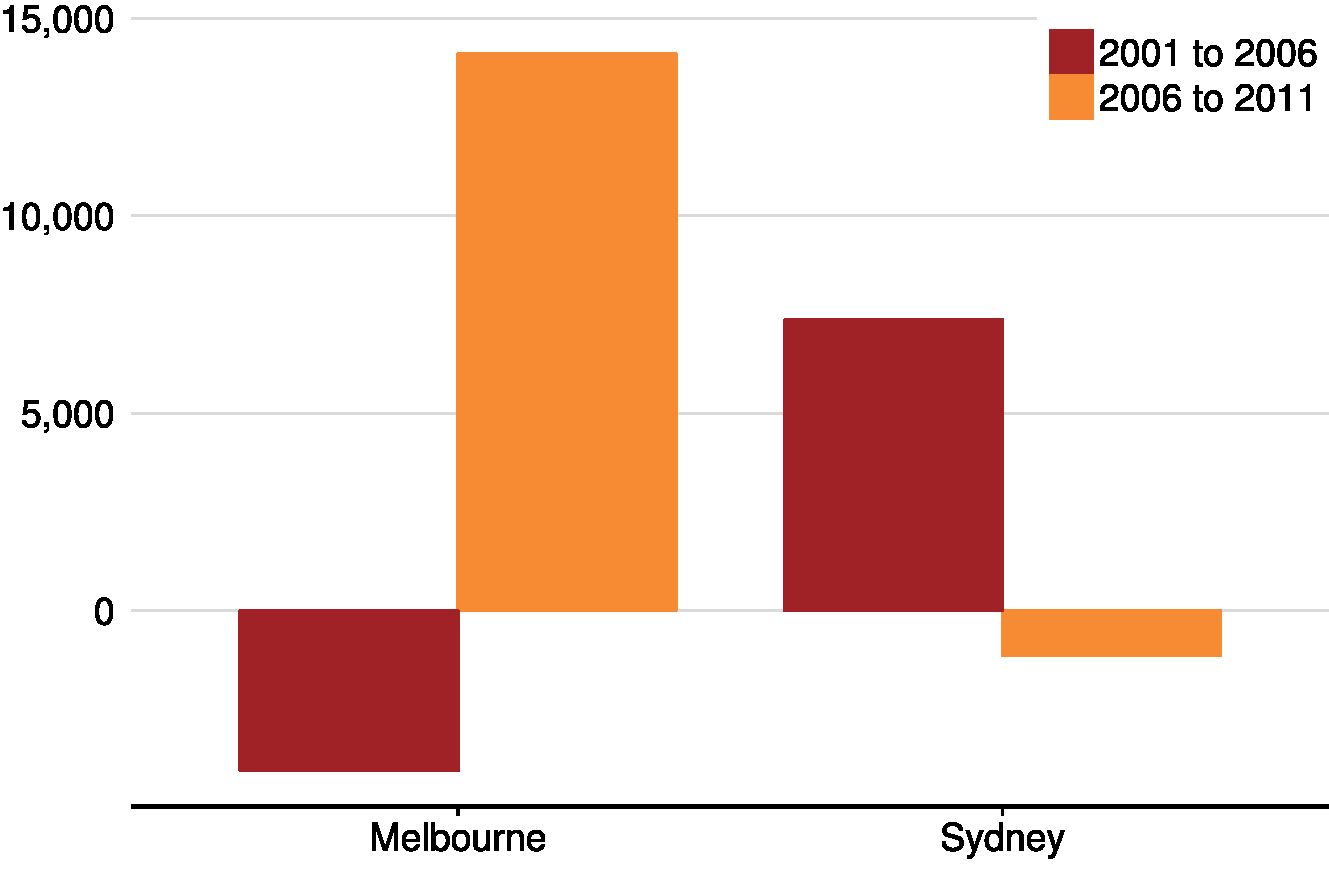
\includegraphics{atlas/absolute-change-in-vehicle-numbers-by-City-year-1.pdf}
\notewithsource{Figures based on 2011 Census, the most recent available at the date of publication}{\textcite{Loader-the-journey-to-work-and-the-city-centre-australian-cities}}
\end{figure}

Melbourne has an expansive public transport network, with more than 830\,km of railway, and the world's biggest tram network.%
    \footcite{PTV-website}
Public transport is relatively cheap in Melbourne; for most commuters, cheaper than in Sydney or Brisbane.%
\footcite{2015-Fare-Benchmarking}

And yet commuting by car to the CBD increased in Melbourne between 2006 and 2011, while it fell in Sydney (\Vref{fig:drivers-to-Melb}). 

The relative attractiveness of driving in Melbourne appears to be caused by two factors: cheap and plentiful parking, and unattractive public transport.
These are undesirable characteristics for a city seeking to ease its most acute congestion.\oneraggedpage
\vfill\null





\subsubsection{There's more parking in Melbourne than Sydney, and it's cheaper}

Melbourne's CBD has 15 per cent more commercial car spaces than Sydney's: around 14.2 spaces per 100 workers in Melbourne, compared with around 12.2 in Sydney.%
    \footnote{\textcite{The-evolution-of-car-parking}. Data on privately-owned non-residential car spaces is not available in a comparable form for Sydney and Melbourne.}

Parking is also much cheaper in Melbourne's CBD than in Sydney's.
All-day early-bird parking in Melbourne costs an average of \$17.74 per day, compared with \$27.74 in Sydney (\Vref{tbl:parking-in-Melbourne-CBD-is-cheap}).
Further, many Melbourne drivers have their parking subsidised or provided by their employer, which tends to make people much more likely to drive to work.%
\footcite{Parking-availability-influences-on-travel-mode}

\begin{table}[!h]
\caption{Parking in Melbourne's centre is cheaper\label{tbl:parking-in-Melbourne-CBD-is-cheap}}
\begin{tabularx}{\linewidth}{lRRRR}
\toprule
              & \textbf{Minimum} & \textbf{Early-bird average} \\
\midrule
Sydney CBD    & \$25.00          & \$27.74 \\
Melbourne CBD & \$15.00          & \$17.74 \\
\bottomrule
\end{tabularx}
\source{\textcite{The-evolution-of-car-parking}}
\end{table}

\begin{figure}
\caption{Melburnians prefer their cars to public transport}\label{fig:marimekko-mode}
\units{Proportion of travel by mode}
% 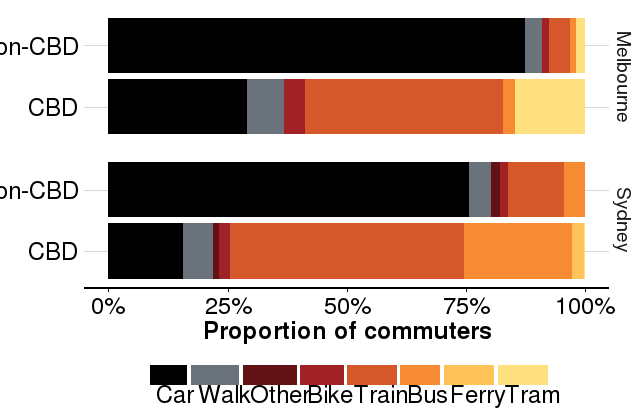
\includegraphics{atlas/Travel-mode-of-CBD-workers-1.pdf}
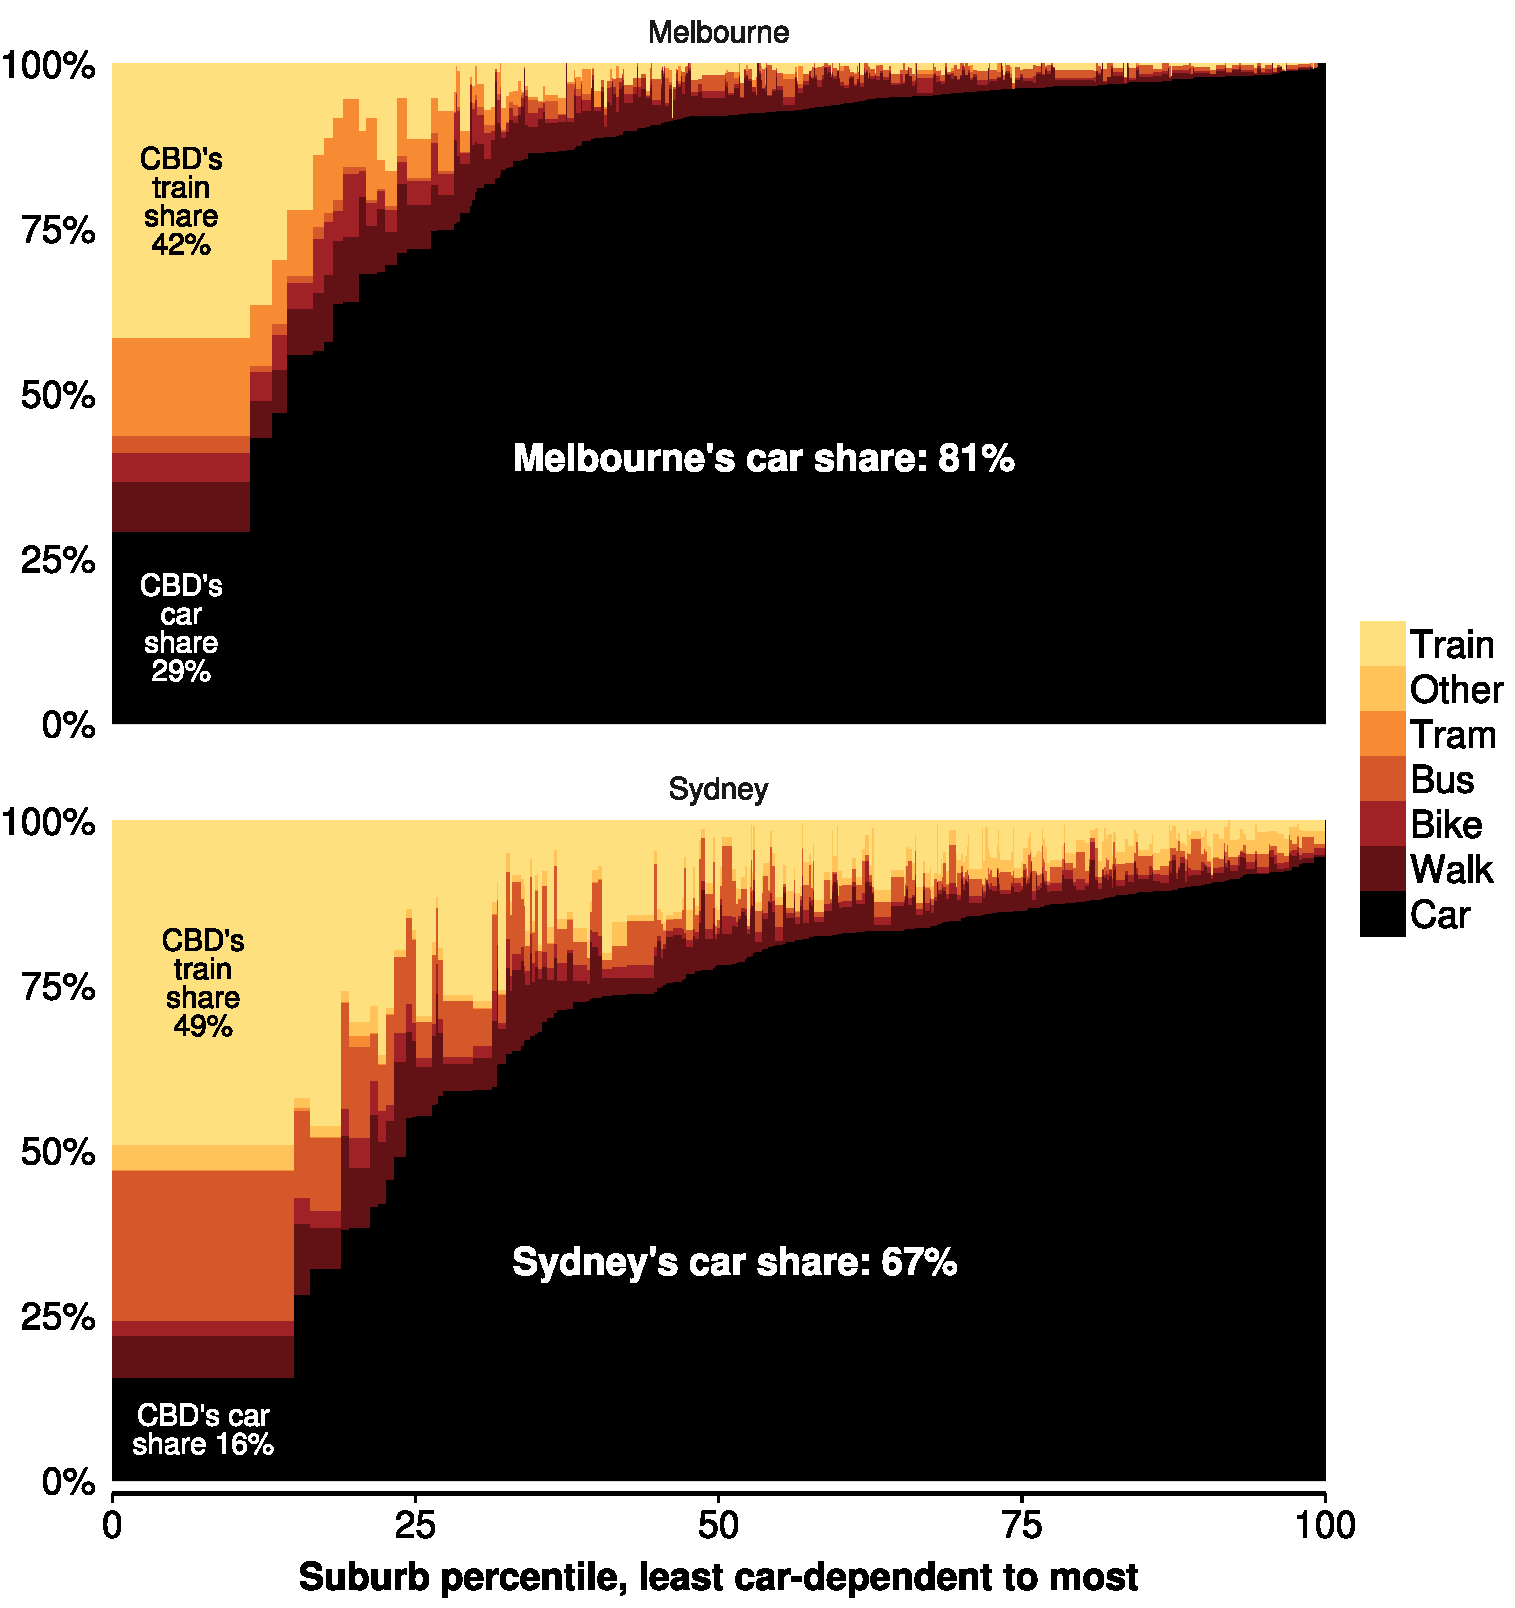
\includegraphics[width=1.14\columnwidth]{atlas/Travel-mode-SYDMEL-1.pdf}
\notewithsource{`Bike' includes bicycle and motorbike.}{Figures based on 2011 Census}
\end{figure}

And the state government-imposed levy on off-street city car parks used by non-residents is \$1380 per year in Melbourne, compared with \$2390 in Sydney.




\subsubsection{Melburnians don't much like commuting by train or bus}

Despite having a big public transport network with relatively cheap fares, Melbourne is highly car-dependent.
Only around 60 per cent of commuters to the CBD use public transport,
compared with over 75~per cent in Sydney.%
    \footcite{ABS2011Census}
For those working outside the CBD, public transport is even less popular (\Cref{fig:marimekko-mode}).

More Melbourne CBD commuters use the train (about 42 per cent) than any other mode of transport.%
\footcite{ABS2011Census}
But for each of the past five years, Melbourne rail passengers have been reporting lower satisfaction than their counterparts in other Australian cities.%
    \footcite{Downes-2016-Metro-trains-pax-ratings}
The main causes of complaints are overcrowding and delays.%
   \footcite{Downes-2016-Metro-trains-pax-ratings}
These concerns are validated by reports from Melbourne's rail operator that more than a quarter of morning peak travellers are affected by overcrowding to the point that there are timetabling delays.%
\footcite{2016-Train-Load-Survey-Report}





Bus patronage is also particularly low in Melbourne.
The combined patronage of buses and trams to Melbourne's CBD is lower than the patronage of buses alone in Sydney.
In fact, commuters to Melbourne's CBD are more likely to cycle than take the bus.%
\footcite{ABS2011Census}
This makes some sense, given that people travelling up to 17 kilometres in Melbourne will arrive home more quickly if they ride a bike than if they take a bus.%
    \footnote{Grattan analysis of \textcite{VISTA}.}


\subsection{Melbourne's toll roads have not been designed to manage congestion}

Melbourne has two toll road networks:  CityLink, which encompasses parts of the Monash and Tullamarine freeways and the Batman Avenue arterial in the city's centre; and EastLink, which connects Nunawading in the east with Frankston in the south-east, providing a link between the Eastern and South Eastern Freeways.
Two more toll roads are planned: the West Gate Tunnel and North East Link.

Melbourne's toll roads offer time savings to motorists who are willing to pay (and hence Google Maps regularly proposes routes that make use of toll roads). The variations in price per kilometre to some extent reflect that the number of minutes saved varies on different toll roads.%
    \footnote{We examined the time savings on trips between the CBD and the following suburbs: Camberwell, South Oakleigh, Dandenong, Frankston, Rowville, Cranbourne, Coburg, Sunbury, Moonee Ponds and the airport.}
In Melbourne, a commuter from the south east to the CBD saves on average 8 to 11 minutes by using CityLink, at a cost of \$8.60.%
    \footnote{This time saving has been calculated by recording the difference between journey times turning on and off Google Maps' ``avoid tolls'' function, for commutes to the CBD from: Dandenong, Cranbourne, Oakleigh South, Rowville and Camberwell.}
This equates to an implied value of time between \$47 and \$65 per hour saved.
Commuters from the airport to the CBD save an average of 8 minutes by using CityLink, at a cost of \$5.60, \ie~an implied value of time of \$42 per hour saved.

As for Sydney, Melbourne's toll roads are not designed to manage congestion.%
    \footnote{The Victorian Government's tolling principles are set out in an appendix to the 2015 Western Distributor business case
    \textcite[][Attachment~F]{Government2015WesternDistributor}.}
Tolls do not vary by time-of-day or levels of congestion, and tolls are not designed to vary in response to changing traffic patterns across Melbourne.



The high levels of congestion on Melbourne's untolled inner-city arterials, such as Punt Road, may arise in part because many drivers do not value their time so highly, preferring to take a slightly slower trip and avoid the toll.%
    \footnote{One factor here may be that many trips on CityLink are undertaken by commercial or business users who place a higher value on their time than commuters or travellers undertaking discretionary trips.
In transport project economic evaluation, it is common to assume a value of time of around \$15 for private vehicles and passengers, \$50 for business travellers, and more than \$100 for some freight vehicles (\textcite{ATAP-2017-Transport-Evaluation-Guidelines}).}

\subsection{Traffic incidents can be disruptive where there are no alternatives}

Accidents, incidents and rain are often blamed for worse-than-usual traffic. Melbourne is less subject to torrential rain than Sydney, and its public infrastructure construction program, while substantial, is smaller.
But of course Melbourne is not immune to incidents and accidents.

On 30~May 2017, a collision between two trucks and a car on the Western Ring Road near Glenroy at 10:25\,am resulted in all four Greensborough-bound lanes being blocked to traffic.
One of the trucks was not righted until 4:30\,pm, and two of the four lanes remained closed until 7\,pm.
It was a big accident, and motorists caught directly behind it endured delays far in excess of Google Maps' estimates. For instance, the evening-peak trip from Footscray to Bundoora using alternative routes took 56 minutes, 13~minutes longer than the normal evening-peak trip.
But for other motorists, the delays were relatively modest.
A trip from Footscray to Bundoora  at 10:30\,am, taking alternative routes, took 37 minutes, just 3 minutes longer than the same trip 30 minutes earlier.

One lesson is that drivers who use navigational-assistance devices to get real-time information can reduce their delays when there is an accident or incident on their normal route.

\chapter{What should we do about it?}\label{chap:what-should-we-do-about-it}

This report has argued that congestion in Sydney and Melbourne is mostly just an irritation for many people much of the time.
But congestion is already sufficiently acute and unpredictable in some places as to warrant a more active policy response. Many of the traditional and easier solutions have already been adopted, particularly in Sydney, and policy reform will become still more pressing as Australia's two largest cities grow.

There are three main policy levers available to manage congestion: investment (new and better roads), pricing (tolls, charges and fares), and government regulation (rules about how we use the roads).
This chapter recommends using the investing and pricing levers, but suggests caution about regulating.

\section{What about new and better roads?}\label{sec:Consider-alternatives-to-building-new-roads}

Despite the claims of politicians, new roads are mostly not ``congestion-busting''.
That's because, when a new road opens, it gets used by people who previously made other choices  -- a different road, a different time, a different mode of travel, or not travelling at all.
The new road offers new possibilities, and people take advantage of them.%
\footnote{This phenomenon is known as ‘induced demand', and has been developed by, among others, \textcites{1991-Small-Urban-transport-economics}{1962-Downs-peak-hour-congestion}.}
This means that, in many cases, congestion levels may be  little changed even after significant new road infrastructure is built, unless drivers face an appropriate price for the congestion they cause.%
    \footcite{Duranton-Turner-2009-Fundamental-Law-of-Road-Congestion}

But it would be a mistake to infer that building new road capacity is always a bad idea. New roads are particularly important to areas where there is new development and population growth.

Of course, new roads are only warranted when the benefits to the community outweigh the costs. But there should be more weighing up of new roads against other options to solve the same problem.%
\footnote{Using a range of recent business cases as a guide, the extent to which this happens at present is limited.
See, for example, \textcite{SGS2016WestConnexreview}.}

New capacity doesn't have to involve big new freeways. It can involve smaller engineering solutions: better intersection design, traffic lighting, accident detection and management systems, improved road surfaces and gradients, lane narrowing, ramp design, and changes to speed limits.
\footcites[][14]{Arnott-Alternatives-to-road-pricing}[][28]{2016-Bertaud}[][29]{2009-queue-duckers}
These smaller solutions have two major attractions: they come into operation much sooner than major new roads could be constructed, and they are far cheaper to build.

To further improve the quality of dialogue between road agencies and the public, state governments should publish more frequent and detailed information about road network performance.
Governments should publish delays for individual roads and routes, to enable better-informed public debate about thresholds for action.
This could include debate about what level of delay is acceptable for different road types and locations.
Governments should also publish information on which roads are near or at their physical capacity at certain times of the day, and plans for managing such constraints.

\section{Make smarter use of pricing}

Pricing should be used much more actively to manage congestion and get the most out of the road network.

It is true that some of the costs motorists pay are like congestion charges: parking fees tend to be higher in congested areas; fuel excise costs are higher for people who spend more time on the road.

But most of the costs motorists pay are not designed to influence congestion.
The upfront cost of owning a vehicle and the costs of registration, a driver's license and insurance are the same regardless of how much the car is driven.
And some of the tax we pay is used to fund new roads, regardless of whether we will ever use those roads.

Motorists also pay tolls to drive on some key roads in Sydney and Melbourne, as mentioned in \Chapref{chap:Congestion-Sydney} and \Chapref{chap:Melbourne-congestion}.
Toll prices vary substantially from one road to another (see \Vref{fig:toll-road-pricing}), depending on factors including where the road is located.

\begin{figure}
\caption{Toll road prices vary significantly across Australia}\label{fig:toll-road-pricing}
\units{Dollars per kilometre  for intracity toll roads}
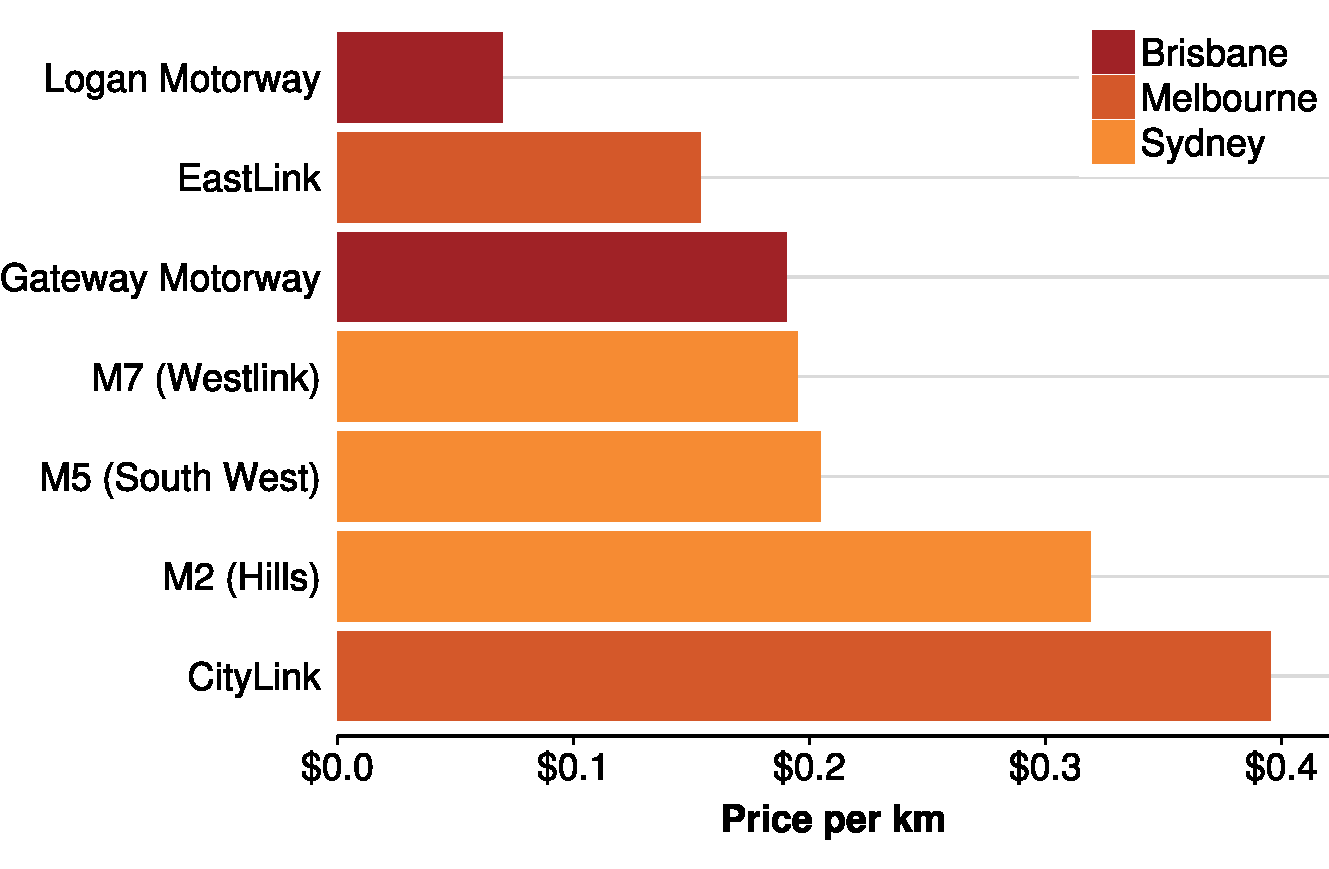
\includegraphics{atlas/TollPrices-freeway-SYD-MEL-1.pdf}
\notewithsource{Grattan analysis based on compilation of intracity toll roads by BITRE as at 31 August 2016.}%
{\textcite{BITRE-toll-roads-in-Australia}.}
\end{figure}

Congestion pricing would be the most effective policy response to congestion in Sydney and Melbourne, and state governments should start planning to introduce it. This will mean a rethink of the way future urban freeways are tolled. In the near term, there remains some low-hanging fruit, mainly for Melbourne: more time-of-day differentiation of public transport fares (lower fares during the shoulder and off-peak periods) and an increase in the CBD parking levy.

\subsection{Establish network-wide time-of-day congestion charging}

With the prospect of further strong population growth, there is a powerful argument for more active network-wide management of congestion.
Improved technologies, already working well overseas, make congestion pricing more feasible now than ever (see \Vref{box:toll-roads-vs-congestion-pricing}).

Network-wide time-of-day pricing schemes should be tailored to Sydney and Melbourne's specific challenges.

The location of congestion in Melbourne suggests more clearly than in Sydney how this might be done, since Melbourne is built on a plain and has a grid-based road network. While imposing a congestion charge on some of the worst roads, such as Hoddle Street, would target some of the worst congestion, it would displace much of the traffic to the adjoining streets. To limit ``rat-running'', we recommend the Victorian Government investigate a ``cordon'' scheme for Melbourne that encompasses key arterials in inner suburbs as well as the CBD\@.
The cordon could cover not only Hoddle Street to the east, but Royal Parade to the west, City Road and Olympic Boulevard to the south, and Alexandra Parade to the north, with motorists charged when they drive across the cordon into the city during peak periods.

For Sydney, the design is less clear. Sydney's intensive economic area extends broadly, and bridges form bottlenecks on some crossings. Nevertheless, the challenges from congestion are becoming significant enough to warrant congestion charging.


\begin{smallbox}{Australian motorists are sensitive to road prices}{box:sensitivity-to-cost-of-tolls}
Australian drivers change their behaviour when tolls are introduced or changed.
When Sydney's Cross City Tunnel opened in 2005, it carried only 20,000 cars a day -- a third of the volumes forecast.
Later, when tolls were lowered, traffic increased to 50,000 cars a day, only to fall again to just above 20,000 when tolls were increased.%
\footcite{Auditor-General-CCT}

Similarly, daily traffic volumes on the Clem7, Brisbane's first road tunnel, fell from 60,000 to 20,000 after tolls were introduced, and then increased when tolls were lowered.
Subsequent changes to tolls also led to noticeable changes in volumes.
A similar pattern was observed on Brisbane's airport link toll road.%
    \footcite{Loader-charting-transport-Traffic-volumes-on-Australian-toll-roads}

Most recently, traffic volumes fell dramatically on Sydney's M4 this year when tolls were reintroduced.%
    \footcite{OSullivan-2017-SMH-New-M4-toll-funnels-more-onto-Parramatta-Rd}
\textcite{Henscher-how-much-is-too-much-for-tolled-road-users} finds that ``toll saturation'' is likely to be increasingly evident in Sydney -- with motorists reaching the limits of what they are able or willing to pay for road use.

Australian motorists' sensitivity to tolls suggests pricing can be a powerful tool for managing congestion. 

\end{smallbox}


For both Melbourne and Sydney, we recommend congestion charges be modest at peak times. Even a low congestion price is likely to persuade some people to change the time, route or mode of their travel, or to decide against taking the trip at all (see \Cref{box:sensitivity-to-cost-of-tolls}).%
\footnote{\textcite{Arnott-Alternatives-to-road-pricing} provides a range of other reasons for congestion pricing to start at very low levels, including the potential impacts on productivity through agglomeration.}

When roads are not congested, the charge should be zero, because a driver using the road at that time does not slow anybody down.


\begin{smallbox}{Building support for congestion charging}{box:building-support-for-congestion-pricing}
Congestion charges tend to be unpopular when proposed, but gain acceptance once imposed.

In Stockholm, Sweden, for instance, congestion charges were unpopular when introduced in 2006, initially for a seven‐month trial.
About 39 per cent of all newspaper articles on the topic were negative, and just 3 per cent positive (the rest were neutral)
    \footcite{congestion-stockholm-trial}
and polling showed public support just before the start of the trial at 34 per cent.
    \footcite{The-Stokholm-Congestion-Charge}
But once the trial started, support for the scheme increased, as residents and commuters benefited from the reduced traffic.
A subsequent referendum was passed, congestion charges were reintroduced in 2007, and by 2014 the scheme was supported by more than two-thirds of the population and all political parties.%
\footcite{The-Stokholm-Congestion-Charge}

In London, the introduction of congestion charges in 2003 (after being championed by Ken Livingston during his successful campaign for Mayor in 2000) was widely resisted.
But acceptance of the scheme increased from about 40 per cent before it was introduced to more than 50 per cent eight months after introduction.%
\footcite{Bhatt-London-Congestion-Charge} Ken Livingston was re-elected Mayor in 2004, and the scheme continues to attract widespread support from both the public and politicians.%
\footcite{The-London-Congestion-Charge}
\end{smallbox}

Congestion charging will be controversial, but has been successfully implemented in other cities worldwide (see \Vref{box:building-support-for-congestion-pricing}).
To reduce the chances of a political backlash, and to emphasise that the charges are designed to ease congestion rather than just to raise revenue, the NSW and Victorian governments should offset congestion charging with discounts on motor vehicle registrations.
And they should consider earmarking the revenues from congestion pricing to spending on public transport.

\subsubsection{Tolling just to raise revenue versus pricing roads to manage congestion}

There is a big difference between tolling roads just to raise revenue, and pricing roads to manage congestion.

The difference lies in what the payment is for.
Congestion prices are not so much about paying for asphalt and traffic lights, but rather charging each driver for their contribution to slowing everyone else down.
Economists seek to do this by paying particular attention to the difference between the private and social costs of road use (see \Vref{subsec:Economists-perspective}).
They find congestion pricing seductive because prices are an instrument that can lift the private cost of a trip up toward the social cost of the trip.
Consequently, carefully set congestion prices nudge traffic flows toward the socially optimal level -- that is, where every driver takes into account their impact on other drivers.

Some policy-makers are more attracted by the revenue-raising possibilities of road tolls than by tolls' ability to nudge drivers' decisions towards the socially optimal level.
Although this is rarely made explicit, they act as if a toll that overshoots the socially optimal level of traffic flow is worthwhile if it achieves higher-order goals such as budget repair.
Important as budget repair may be, a congestion charge that overshoots the social optimum is best thought of as a tax, and, given that people seem very responsive to road prices (\Cref{box:sensitivity-to-cost-of-tolls}), a very distorting tax.
\footcites[][17]{HenryTaxReview2010}{KPMGEcontech2010-CGE-Analysis-of-Current-Aust-Tax-System}

In any case, well-designed congestion charges are likely to raise significant revenue without exceeding the socially optimal level.%
\footnote{According to the Mohring-Harwitz theorem, a congestion charge set at a level equal to the congestion externality would raise enough revenue to cover the total costs of constructing and maintaining the roads: \textcite{2007-Mohring-Harwitz-theorem}.} %

\subsection{Build in flexibility to change prices as congestion changes}

The introduction of congestion charging will mean that governments take a different approach to future toll roads.

The NSW and Victorian governments at present hold very long-term contracts with private toll operators. For example, tolling arrangements for the new WestConnex freeways in Sydney will be in place until at least 2060.%
    \footcite{Ken-Kanofski-NSW-Legislative-Council-Inquiry-Road-Tolling-responses-to-supplementary-questions}
This practice reduces government's flexibility to manage congestion over time.
And as the number of toll roads increases, the likelihood that future toll prices will need to be re-calibrated increases.

Tolling principles in both NSW and Victoria acknowledge that it is desirable to set tolls with reference to their broader impact on the rest of the road network.
But in reality, it appears congestion management is at best a minor consideration. Peak period pricing was not proposed in the Victorian Government's Western Distributor business case, for example, because it was deemed inconsistent with existing arrangements on CityLink.%
    \footcite[][108]{Government2015WesternDistributor}
In Sydney, too, the peer review of the WestConnex business case noted there was no detailed examination of the link between travel-time savings and toll prices.%
    \footcite[][39]{SGS2016WestConnexreview}

It is impossible to predict with confidence how the road network will be used in the medium and longer term.
If traffic forecasts turn out to be wrong -- as they have been many times in the past -- then it is valuable to have the flexibility to adjust toll prices to better manage the network as a whole.

It is true that future toll prices can be adjusted via contract variations to tolling concessions. But the cost of such variations is likely to be very high, and borne by taxpayers. Additional complexities surrounding contract variations will also surface -- for example, Victoria's Western Distributor business case notes that any proposed change to the tolling structure would require reconsideration of the CityLink tolling structure (which may come to be owned by separate private sector operators).%
    \footcite[][113]{Government2015WesternDistributor}

Governments can best achieve greater flexibility to adjust future toll prices to better manage the road network by retaining toll revenues from future tolled roads as government revenue.
A potential downside, given road tolling is a politically charged issue, is that politicians may be tempted to change toll prices for political gain.
To avoid this risk, we recommend vesting the management of toll roads, and the setting of toll prices, in an independent government regulatory body such as the Independent Pricing and Regulatory Tribunal (IPART) in NSW, the Essential Services Commission in Victoria, or the Australian Competition and Consumer Commission.



\begin{bigbox*}{Road-user charging overseas -- some schemes price congestion, others target revenue}{box:toll-roads-vs-congestion-pricing}
Road pricing is gathering support around the world.
In some cases, the impetus is concern about urban congestion.
In other cases, it stems from the need to replace declining revenues from existing road-related taxes and charges, such as fuel excise, or a more general desire to raise revenue.


One of the best-known schemes to manage congestion is London's cordon scheme, introduced in 2003. Motorists pay up to £11.50 (\$19AUD) when they cross a boundary that marks a central city zone. The number of cars entering central London has fallen by nearly a quarter since 2000.%
	\footcite{TheEconomist-2017-Road-pricing-has-long-been-a-good-idea}
But the gains in travel speeds are slowly diminishing, due to steadily growing traffic volumes and an inherent limitation of cordon schemes -- vehicles that stay inside the zone are not charged, making it free for them to cruise the inner London streets.
London authorities are now considering how to redesign the scheme so motorists are charged according to when, where and how much they use the roads.

London is likely to look to Singapore, which has the world's most comprehensive congestion charging scheme -- applying prices that vary throughout the day with the goal of eliminating flow breakdowns and ensuring roads operate at their capacity.%
    \footcite[][22]{Wallis-Lupton-2013-NZ-Transport-Agency}
Singapore's scheme has relied on numerous gantries to detect and capture vehicle movements, but is increasingly using Global Navigation Satellite System technology.
The goal is to extend the scheme to the entire island by 2020.

By contrast to London and Singapore, several schemes in the US focus on revenue-raising.
``Pay to drive'' schemes are being tested in Oregon, California and Colorado.
In the Oregon trial, which started in 2015, cars are fitted with a device that takes data from the engines' computers.
Drivers are charged 1.5~cents a mile, regardless of where they are travelling or whether there is any congestion when they do.

In Australia, toll roads have been established with a focus on revenue-raising, not congestion-management.
The only toll roads in Australia with prices varying by time-of-day and day-of-week for private passenger vehicles are on the Sydney Harbour Bridge and Tunnel.
\footcite{BITRE-toll-roads-in-Australia}

\boxsources{\textcite{TheEconomist-2017-Road-pricing-has-long-been-a-good-idea}}
\end{bigbox*}

\subsection{`Low-hanging fruit' options for Melbourne}
With its larger population, Sydney has already adopted some successful strategies to manage congestion. Melbourne should adopt two of these in the next 12 months: more time-of-day differentiation of public transport fares, and increasing the CBD parking levy.
\subsubsection{Differentiate public transport fares more by time of day}

Even though most trips are by car, public transport is still an important part of the transport network.
It is most efficient at moving large numbers of people going to the same place.

Sydney has done more than Melbourne to create incentives for public transport use to move to quieter times by charging higher fares during peak periods.
But it should do more still.

In the short term, the NSW Government should adopt a recent recommendation from IPART and make a bigger cut to off-peak fares.%
    \footnote{In May 2016, the NSW Government rejected IPART's recommendation that the off-peak discount on trains be increased from 30 per cent to 40 per cent.}
Over the longer term, the NSW Government should introduce an even wider range of time-dependent fares, including new ``shoulder'' fares that sit between the peak and off-peak fares.

The spirit of these recommendations applies with greater force to Melbourne, where fares are less variable than Sydney's.
Melbourne currently offers free rail travel for trips that terminate before 7:15\,am, and people who start a journey after 6\,pm can use their short-term ticket for travel until 3\,am the following day.
\Vref{fig:PTV_loads} shows the high concentration of train use in Melbourne at peak times of day. Much more should be done to encourage people who have the flexibility to shift their travel from peak to off-peak periods to take advantage of spare capacity at those times. 

\begin{figure}
\caption{Public transport use is highly concentrated at peak periods}\label{fig:PTV_loads} % should not be a line chart
\units{Average half-hourly weekday train boardings on Melbourne public transport}
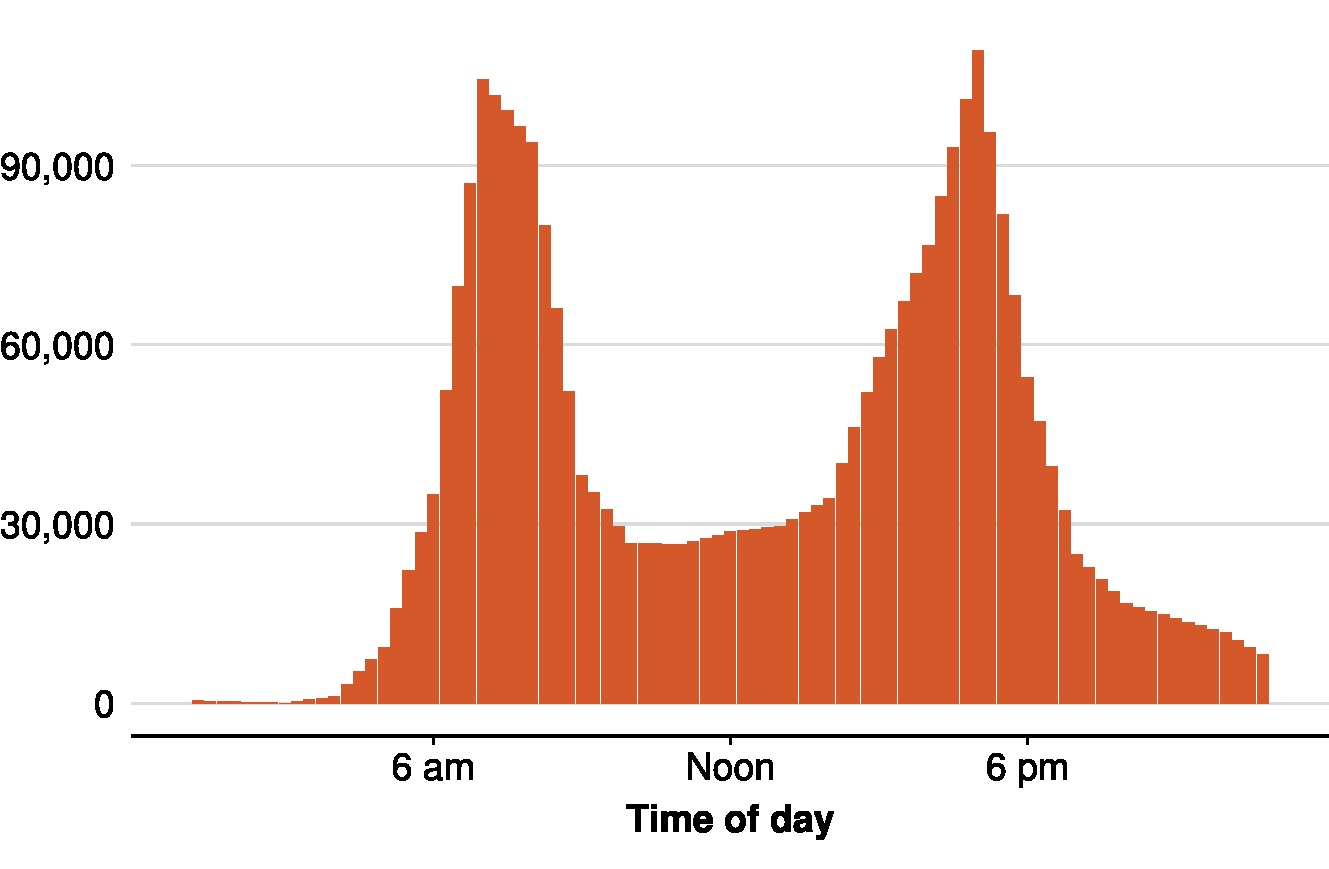
\includegraphics{atlas/Public-transport-use-1.pdf}
\source{PTV/VicRoads, unpublished}
\end{figure}

But ultimately, the best way to enhance the attractiveness of public transport is to introduce a road congestion charge -- especially to improve travel times on buses and trams.%
    \footcite{Urbanist-2011-Do-governments-spend-too-much-on-roads}

\subsubsection{More expensive parking in Melbourne's inner city}
Parking is more attractive in Melbourne than Sydney: it's generally cheaper, and there are more commercial spaces available relative to the number of CBD workers.

Melbourne's parking levy is around half the cost of Sydney's.
The Victorian Government should increase it, to match Sydney's.
A levy on city parking can be thought of as a form of congestion charging, because it encourages drivers who cause congestion to either change their mode of travel or pay an increased price.
Unlike most taxes, the parking levy is an attractive instrument for governments because it helps to better align the incentive to drive with the full costs to the community of one person driving.

Levies on city parking affect not only the incentives of individual motorists but also the incentives of employers, who may decide to cash out their employee car parking benefits if the levy is increased.

A levy increase in Melbourne would be easy to implement and would have no additional administration costs.
On its own it would not have an overwhelming impact on congestion, but it would be a useful interim measure before the introduction of congestion pricing.
The extra revenue from an increased levy could be directed to improving public transport.


\section{A limited role for regulation}\label{sec:Regulations}

\begin{figure}[p]
\caption{Public holidays make a difference to congestion, school holidays not so much}\label{fig:congestion-school-holidays}
\units{Average effect of day-of-week and holidays on trip time}
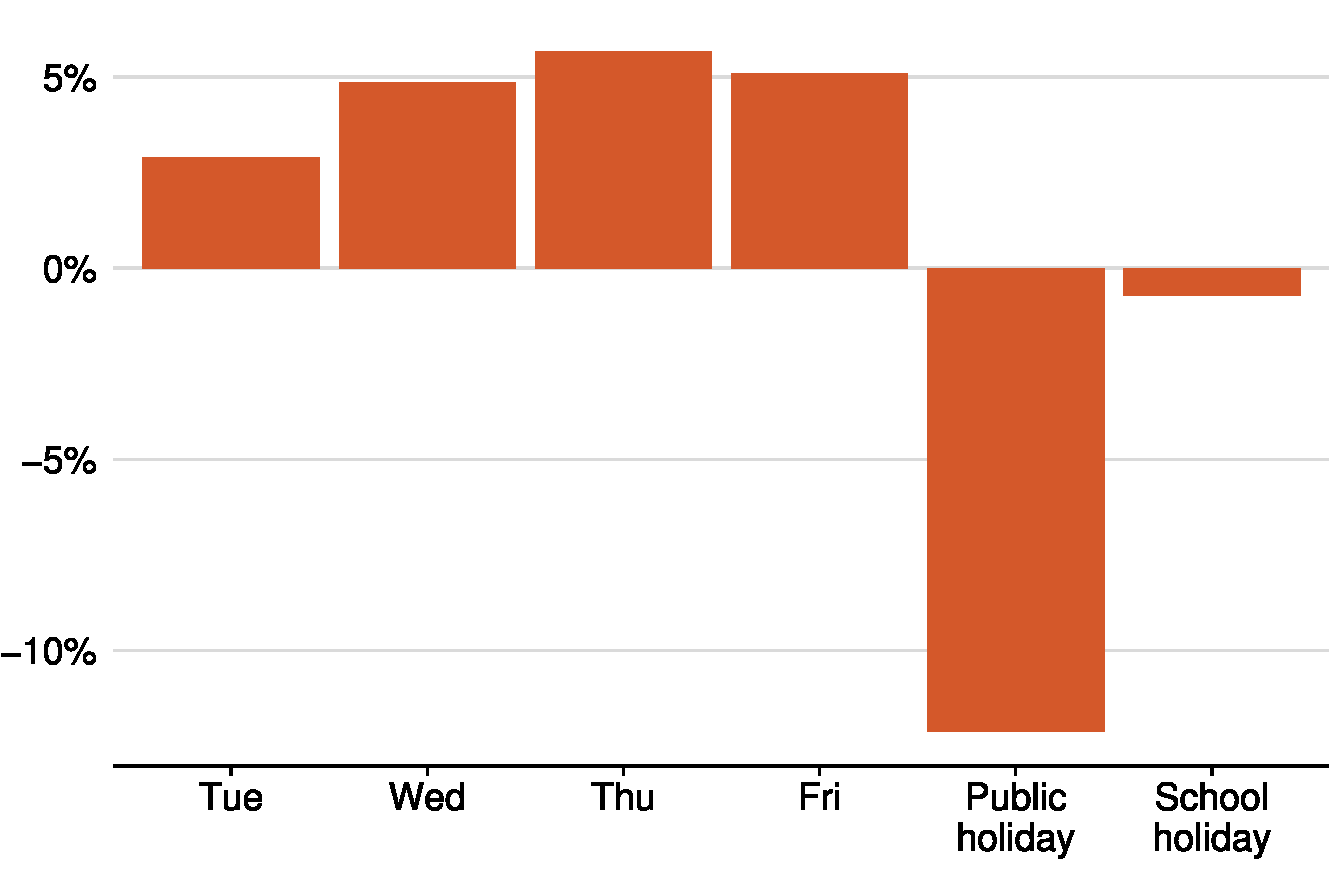
\includegraphics{atlas/simpleModelPlot-1.pdf}
\noteswithsource{Linear model of peak trip duration for each morning and afternoon sampled, controlling for origin-destination and time of day.
Estimates are with respect to non-holiday Monday mornings.}%
{Grattan analysis of Google Maps.}
\end{figure}

Governments can also use regulations to ease congestion. Regulatory solutions range from the incremental (such as limiting parking, implementing clearways and banning right-hand turns) to the heavy-handed (such as mandating individuals only drive on certain days,%
    \footnote{This policy has been implemented in many cities, including Paris, Athens, Delhi, São Paulo, Beijing and Mexico City.
Vehicles may not be driven on certain days based on the last digit on their number plate.
Such policies have generally been implemented to reduce air pollution but could be used to target congestion.}
requiring private vehicles to carry a certain number of passengers,%
    \footnote{For example, Jakarta’s “three-in-one" policy required a minimum of three passengers before a vehicle could travel on some major roads  or in peak periods. \textcite{HOV-Jakarta}.}
or staggering start times for schools and jobs).
Regulations that discourage aggressive driving can make travel more enjoyable, and hence less costly -- although this in itself can bring more people onto the roads.%
\footcite[][10--11]{Arnott-2001-Microscopic-research-agenda}

We recommend the NSW and Victorian governments expand incremental regulatory measures.
For example, limiting the amount of on-street parking and banning right-hand turns in congested areas would reduce the attractiveness of driving there and could improve traffic flows, particularly on busy arterials.

But we are wary of heavy-handed, system-wide regulations. The \textcite{NRMA-SchoolHolidays-2013} claims that road speeds in Sydney increase by at least 50~per cent during school holidays, which is often cited as a reason to promote flexible working hours or staggering school start time to address congestion.



Our analysis does not support this claim.
Congestion during the Easter and mid-year school holidays of 2017, whether measured using speed or trip duration, was no different to congestion during the school term -- in both Melbourne and Sydney.
Public holidays were associated with a 10~per cent reduction in travel times; school holidays barely registered (\Vref{fig:congestion-school-holidays}).

While some trips are quicker during school holidays -- such as, unsurprisingly, trips to and from schools in local communities -- our analysis does not support the idea that changing school hours will substantially ease road congestion.

Therefore we do not recommend the popular idea of staggering school start times to reduce congestion, or any of the other heavy-handed solutions which have created unintended costs overseas.%
    \footnote{For example, Mexico’s number-plate policy resulted in increased car sales; Jakarta's “three-in-one” policy resulted in a market where people could ``buy'' passengers to ride in their car (\textcite{congestion-Mexico-cityl}).}


















\newcolumntype{N}{l@{}}
%\onecolumn
\appendix
\chapter{Defining congestion}\label{chap:appendix-defining-congestion}

Roads are “congested” when the number of vehicles using them causes unacceptable levels of discomfort and delay.%
    \footcite[][93]{Falcocchio-and-Levinson-congestion-a-concise-guide}
But of course “unacceptable” means different things to different people. Three different perspectives – those of motorists, engineers, and economists -- provide definitions that can help policy-makers.%
    \footcite[][7]{Wallis-Lupton-2013-NZ-Transport-Agency}

\phantomsection
\label{para:three-perspectives-on-congestion--intro}
\zlabel{para:three-perspectives-on-congestion--intro}
The three perspectives are set out below.

\section{Motorists care about travel time and reliability}\label{subsec:road-users-perspective}
For motorists, a road is too congested if their speeds drop too far and their trip takes too much longer than expected. Expected travel time is subjective, and depends on location, time of day, and type of road. The motorist's perspective is sometimes referred to as “perceived” congestion.%
    \footcite[][108]{Falcocchio-and-Levinson-congestion-a-concise-guide}

The main way to assess congestion from the motorist's perspective is to compare travel times when there is congestion with travel times for the same trip when there is no congestion – usually in the middle of the night.

This measure is useful for policy-makers only when comparing congestion across cities of similar sizes.
This is because the economic cost of congestion depends on the size of the city.
If a trip takes 50 per cent longer in peak hour than it would in the middle of the night, the economic costs it imposes will be larger in a city that has longer average trip lengths and more people taking the trip – \ie~in larger cities.

So comparing Sydney with Melbourne is much more useful than comparing Sydney with, say, Canberra.

Reliability is also important to motorists; the predictability of a trip's time determines how much of a buffer people need to leave if they have to arrive at their destination by a specific time.

\section{Engineers care about a road's physical capacity}\label{subsec:engineers-perspective}
Traffic engineers consider a road congested when more vehicles are attempting to use the road than it has physical capacity to carry.%
    \footcite[][7]{Wallis-Lupton-2013-NZ-Transport-Agency}
Capacity refers to the maximum number of vehicles the road is capable of carrying over a fixed period – the maximum possible throughput.

When traffic flows are moderate, more vehicles can enter the stream of traffic and the overall throughput of the road can keep increasing.
But there comes a point where more vehicles entering the stream of traffic leads to a crop in overall throughput: when individual vehicles slow down to deal with all the other vehicles braking, changing lane and sharing the road space.

\begin{figureTop}
\caption{Optimal traffic levels depend on the relationship between throughput, density and speed}\label{fig:Arnott-flow-curves}
\units{Traffic throughput (\eg~vehicles per hour), density (\eg~vehicles per 100 meters of road) and speed (\eg~\kmh)}
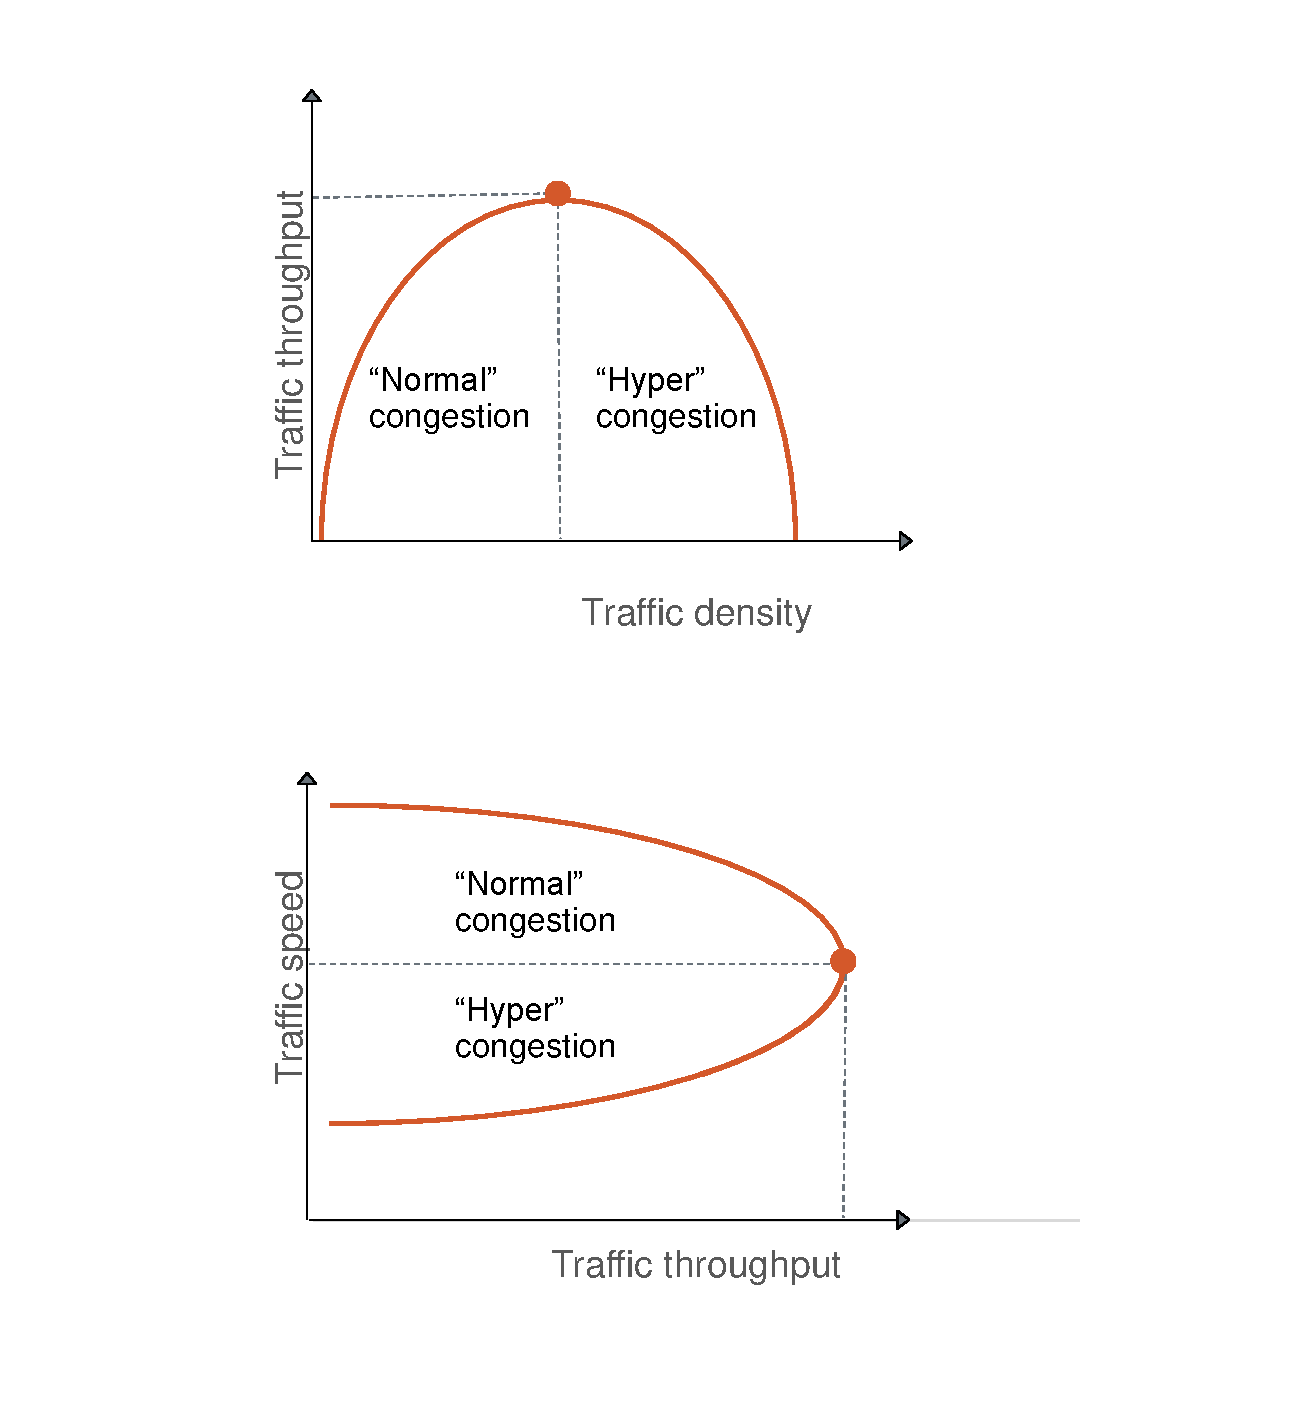
\includegraphics[page=1]{Charts/ChartPackLong.pdf}
\noteswithsource{These curves present the theoretical relationship between these variables. \textcite{Chavis-etal-2011-Multimodal-transport-Nairobi} provide empirical evidence for this relationship using data from a range of cities internationally.}{\textcites[][29]{Arnott-2015-Bathtub-model-of-traffic-congestion}{Austroads-2015-Guide-Traffic-Mgmt}}
\end{figureTop}

The first curve in \Vref{fig:Arnott-flow-curves} shows traffic throughput initially increasing with greater traffic density, but eventually decreasing as the number of vehicles on the road becomes too high.

The second curve in \Cref{fig:Arnott-flow-curves} tells a similar story.
Reading the curve clockwise, speed gradually falls as traffic density increases.
But throughput continues to increase up to a certain point (the ``bullet nose'' of the curve), after which speed and throughput both decline.

The first half of each curve in \Cref{fig:Arnott-flow-curves} shows “normal” congestion.
The second half shows ``hyper'' congestion: the road is being used beyond its capacity.

Each time a vehicle joins a road, it slows everyone else.
This can impose a cost on the other motorists, even before the road becomes hyper-congested.
The following section focuses on this way of viewing congestion.


\section{Economists care about how the value of trips compares with the costs those trips impose on everyone} \label{subsec:Economists-perspective}

Economists focus on the costs and benefits that road users experience at different levels of traffic flow.
They pay particular attention to the difference between the private cost of an additional trip and the social cost of that trip.

\begin{itemize}
\item The private cost is incurred by the person who takes the trip, and includes tolls, the cost of fuel, the cost of wear and tear on a car and the value to the person of the time taken to make the trip.
\item The social cost is the private cost \textbf{plus} the cost that the trip may impose on \textbf{others}, mainly in the form of the time added to the trips of every other road user.%
\footnote{The social cost excludes any tolls, because they are transfers to another party.
As well as congestion, social costs include pollution and accidents.}
\end{itemize}

Economists will see ``excessive'' congestion well before engineers do; it is not hard to imagine that, when a road is busy, the social cost of a trip may be much higher than the private cost of a trip (\Vref{box:explaining-congestion-as-negative-externality}).

\phantomsection
\label{para:three-perspectives-on-congestion--end}



\chapter{About the data}\label{chap:appendix-notes-on-sample}
The primary data source for this report consists of trip time estimates for approximately 350 origin-destination pairs in Sydney, Melbourne, and Brisbane, made available by Google. Census data is also used.%
\footnote{At the time of publication, the most recent data on journeys to work was from the 2011 Census.}

\section{About Google Maps}
Google provides an Application Programming Interface to its `Distance Matrix' service, which returns an estimate of trip duration and distance in response to a query.

The Distance Matrix is proprietary, so neither its source code nor broad, reliable measures of its accuracy are publicly known.
Its estimates likely draw on sources including posted speed limits, actual travel times from previous users, and real-time and historical traffic information from road authorities and telecommunications metadata.

We regard the estimates as reliable.
The market for high-accuracy estimates of trip times is competitive and mature.
In addition, high-quality data that could be used to provide accurate estimates of trip times and traffic conditions, while requiring extraordinary resources, is available in high volumes.
The popularity of Google Maps is good evidence that estimates from its API are the best publicly available.

\section{About the sample}

The 350 origin-destination pairs were chosen to provide insight to a number of different journeys (such as CBD commutes, commutes to other employment destinations, cross-city journeys, local journeys and leisure trips) within Australia's major cities.
They do not represent every trip that motorists may take.

Trip time estimates for these 350 core trips were collected 25 times a day (at 15-minute intervals during the peak and hourly or 2-hourly off-peak),
 between March and September 2017, using the API.

During this time, extra routes were added to the sample to enable more in-depth analysis.
These included routes along arterial roads, which we used to analyse the level of service of particular roads; journeys to work that replicate the journeys reported in the 2011 Census; and a comparison of tolled and untolled route options for particular origin-destination pairs using the ``avoid tolls" function.

\section{Limitations of the data for this analysis}
Google's Terms of Service prohibit storing or analysing data returned by the Distance Matrix (Grattan Institute obtained an exemption from this clause).
While we believe the estimates to be reliable, they were not produced for research purposes.

Estimates returned by the Distance Matrix may not reflect the actual time taken.
In particular, an estimate of trip duration only applies when the trip is started.
At one extreme, if an accident occurred in the M5 tunnel near Sydney Airport, drivers already on the freeway may have no option but to wait until the accident is cleared.
Yet the estimates from the Distance Matrix at the time have the option to avoid the tunnel, thus masking the experience of those in the tunnel.

There are other minor curiosities too.
For example, estimates do not always satisfy the triangle inequality.
That is, the estimated trip time from A to~B may be longer than the sum of trip times of A to~C and C to~B.

Furthermore, queries were sent using an origin and destination address, but since the API interprets these addresses it can also misinterpret them -- either the origin or destination actually used may be wrong and provide a spurious estimate.
We excluded observations that were clearly misinterpreted, but this filter would not detect all errors of this kind.





% One column will place the chapter titles differently
\onecolumn\vtop to 0pt\bgroup\vspace{-24.5pt}\chapter{Routes sampled}\label{chap:Routes-sampled}\egroup\vspace{\baselineskip}
% latex table generated in R 3.4.0 by xtable 1.8-2 package
% Sat Jul 29 03:02:30 2017
\begin{longtable}{Nlllrr}
\caption{Melbourne routes}\label{tbl:Melbourne-classification-table} \\
\toprule
\textbf{\phantom{\null}} & \textbf{Classification} & \textbf{Origin} & \textbf{Destination} & \textbf{Days sampled} & \textbf{Min. trip time (mins)} \\
\midrule
\endfirsthead
\caption*{Table \thetable: \nameref{tbl:Melbourne-classification-table}  (continued)} \\
\toprule
\textbf{\phantom{\null}} & \textbf{Classification} & \textbf{Origin} & \textbf{Destination} & \textbf{Days sampled} & \textbf{Min. trip time (mins)} \\
  \midrule
\endhead
\bottomrule
\multicolumn{6}{>{\footnotesize\itshape\arraybackslash}r}{Continued on next page}
\endfoot
\bottomrule
\endlastfoot
 & CBD commuting                  & Melbourne CBD           & Brighton                 & 160 & 17:06 \\
 &                                &                         & Camberwell               & 160 & 16:05 \\
 &                                &                         & Caroline Springs         & 160 & 25:56 \\
 &                                &                         & Coburg                   & 160 & 19:41 \\
 &                                &                         & Craigieburn              & 107 & 38:00 \\
 &                                &                         & Cranbourne               & 160 & 38:49 \\
 &                                &                         & Dandenong                & 160 & 27:28 \\
 &                                &                         & Diamond Creek            & 107 & 34:11 \\
 &                                &                         & Doncaster                & 160 & 18:39 \\
 &                                &                         & Donnybrook               & 60  & 39:58 \\
 &                                &                         & Footscray                & 107 & 14:46 \\
 &                                &                         & Frankston                & 107 & 40:33 \\
 &                                &                         & Heidelberg               & 160 & 17:33 \\
 &                                &                         & Hoppers Crossing         & 160 & 28:34 \\
 &                                &                         & Kew                      & 107 & 13:17 \\
 &                                &                         & Melbourne Airport        & 160 & 25:55 \\
 &                                &                         & Moonee Ponds             & 107 & 17:07 \\
 &                                &                         & Oakleigh South           & 160 & 20:27 \\
 &                                &                         & Port Melbourne           & 160 & 10:39 \\
 &                                &                         & Rowville                 & 160 & 25:54 \\
 &                                &                         & Sunbury                  & 107 & 36:19 \\
 &                                &                         & Sunshine West            & 160 & 20:21 \\
  \multicolumn{4}{@{}l@{}}{\null}\\[-8pt]
 & Capacity tester -- arterial    & Keilor East             & Sunshine                 & 60  & 10:46 \\
 &                                & Preston                 & Preston                  & 93  & 3:15 \\
 &                                & Vermont South           & Glen Waverley            & 93  & 3:39 \\
 &                                & Watsonia                & Macleod                  & 93  & 2:46 \\
  %\multicolumn{4}{@{}l@{}}{\null}\\[-10pt]
 & Capacity tester -- freeway     & Box Hill North          & Nunawading               & 93  & 4:31 \\*
 &                                & Glen Iris               & Mount Waverley           & 93  & 7:33 \\
 &                                & Port Melbourne          & Spotswood                & 93  & 5:37 \\
  \multicolumn{4}{@{}l@{}}{\null}\\[-10pt]
 & Cross city                     & Richmond                & Essendon                 & 165 & 22:40 \\
 &                                & Footscray               & Richmond                 & 165 & 19:09 \\
 &                                & Hawthorn                & Northern Hospital Epping & 165 & 33:24 \\
 &                                & Point Cook              & Glen Waverley            & 165 & 39:02 \\
  \multicolumn{4}{@{}l@{}}{\null}\\[-10pt]
 & Freight                        & West Melbourne Port     & Altona                   & 155 & 18:43 \\
 &                                &                         & Bacchus Marsh            & 155 & 40:47 \\
 &                                &                         & Dandenong                & 155 & 33:38 \\
 &                                &                         & Somerton                 & 155 & 24:12 \\
 &                                &                         & Truganina                & 146 & 23:16 \\
 &                                & Melbourne Airport       & Dandenong                & 162 & 47:13 \\
 &                                &                         & Northern Hospital Epping & 162 & 18:49 \\
  \multicolumn{4}{@{}l@{}}{\null}\\[-10pt]
 & Hotspot                        & Cranbourne North        & Berwick                  & 141 & 8:55 \\
 &                                & Mernda                  & South Morang             & 139 & 10:33 \\
 &                                & Parkville               & Coburg Library           & 141 & 10:22 \\
 &                                & Seaford                 & Carrum Downs             & 141 & 9:00 \\
  \multicolumn{4}{@{}l@{}}{\null}\\[-10pt]
 & Inner suburb short trip        & Melbourne CBD           & Carlton                  & 162 & 4:35 \\
 &                                & Richmond                & South Yarra              & 162 & 4:24 \\
 &                                & Clifton Hill            & Prahran                  & 162 & 12:05 \\
 &                                & Southbank               & South Yarra              & 162 & 8:01 \\
  \multicolumn{4}{@{}l@{}}{\null}\\[-10pt]
 & Leisure trip                   & Melbourne CBD           & North Fitzroy            & 162 & 10:09 \\
 &                                & Albert Park             & Melbourne CBD            & 162 & 8:28 \\
 &                                &                         & Preston                  & 162 & 24:20 \\
 &                                & Richmond                & Keilor                   & 162 & 23:34 \\
 &                                &                         & Seaford                  & 162 & 34:42 \\
 &                                & Braybrook               & Carlton                  & 162 & 15:38 \\
 &                                & Chadstone               & Bentleigh                & 162 & 11:51 \\
 &                                & Maribrynong             & Sunshine                 & 162 & 8:19 \\
 &                                & Mornington              & Melbourne CBD            & 162 & 52:09 \\
 &                                & South Yarra             & St Kilda                 & 162 & 7:17 \\
  \multicolumn{4}{@{}l@{}}{\null}\\[-10pt]
 & Middle ring short trip         & Caulfield racecourse    & St Kilda baths           & 162 & 10:19 \\
 &                                & Chadstone               & Blackburn station        & 162 & 17:10 \\
 &                                & Clayton                 & Monash Medical Centre    & 162 & 5:48 \\
 &                                & Maribrynong             & Keilor East              & 162 & 6:02 \\
 &                                & Moonee Ponds            & Essendon DFO             & 162 & 7:32 \\
 &                                & West Footscray          & Yarraville               & 141 & 7:10 \\
  \multicolumn{4}{@{}l@{}}{\null}\\[-10pt]
 & Non-CBD employment centre trip & Box Hill                & Preston                  & 162 & 23:20 \\
 &                                & Bundoora                & Footscray                & 164 & 30:26 \\
 &                                & Clayton                 & Frankston                & 162 & 24:47 \\
 &                                & Collingwood             & Essendon                 & 162 & 19:32 \\
 &                                & Docklands               & Blackburn                & 162 & 28:43 \\
 &                                & Fitzroy                 & Clayton                  & 162 & 25:47 \\
 &                                & Flemington              & East Kew                 & 162 & 17:41 \\
 &                                & Melbourne Uni           & Williamstown             & 162 & 22:04 \\
 &                                & South Yarra             & Kew                      & 162 & 12:52 \\
 &                                & West Melbourne          & Richmond                 & 162 & 11:40 \\
 &                                & Yarraville              & St Kilda                 & 162 & 18:51 \\
  \multicolumn{4}{@{}l@{}}{\null}\\[-10pt]
 & Outer areas short trip         & Berwick                 & Dandenong                & 162 & 16:07 \\
 &                                &                         & Dandenong North          & 141 & 16:42 \\
 &                                & Deer Park               & St Albans                & 162 & 5:06 \\
 &                                & Montrose Primary School & Lilydale High School     & 162 & 9:43 \\
  \end{longtable}

\clearpage
\null\vspace{\baselineskip}
%!TeX Root=../Report.tex
% latex table generated in R 3.4.0 by xtable 1.8-2 package
% Sat Jul 29 10:25:32 2017
\begin{longtable}{Nlllrr}
\caption{Sydney routes}\label{tbl:Sydney-classification-table} \\
\toprule
\textbf{\phantom{\null}} & \textbf{Classification} & \textbf{Origin} & \textbf{Destination} & \textbf{Days sampled} & \textbf{Min. trip time (mins)} \\
\midrule
\endfirsthead
\caption*{Table \thetable: \nameref{tbl:Sydney-classification-table}  (continued)} \\
\toprule
\textbf{\phantom{\null}} & \textbf{Classification} & \textbf{Origin} & \textbf{Destination} & \textbf{Days sampled} & \textbf{Min. trip time (mins)} \\
  \midrule
\endhead
\bottomrule
\multicolumn{6}{>{\footnotesize\itshape\arraybackslash}r}{Continued on next page}
\endfoot
\bottomrule
\endlastfoot
 & CBD commuting                  & Sydney CBD            & Artarmon             & 165 & 12:17 \\
 &                                &                       & Blacktown            & 165 & 35:50 \\
 &                                &                       & Bondi Beach          & 152 & 15:44 \\
 &                                &                       & Campbelltown         & 165 & 44:04 \\
 &                                &                       & Castle Hill          & 165 & 29:19 \\
 &                                &                       & Coogee               & 152 & 14:08 \\
 &                                &                       & Cronulla             & 165 & 32:24 \\
 &                                &                       & Gosford              & 165 & 60:06 \\
 &                                &                       & Hornsby              & 165 & 28:45 \\
 &                                &                       & Hurstville           & 165 & 25:11 \\
 &                                &                       & Liverpool            & 165 & 34:12 \\
 &                                &                       & Macquarie Park       & 165 & 17:25 \\
 &                                &                       & Manly                & 162 & 24:11 \\
 &                                &                       & Marrickville         & 165 & 17:12 \\
 &                                &                       & Mona Vale            & 165 & 36:56 \\
 &                                &                       & Mosman               & 152 & 12:10 \\
 &                                &                       & Penrith              & 165 & 50:26 \\
 &                                &                       & Ryde                 & 165 & 18:25 \\
 &                                &                       & Sydney Airport       & 165 & 12:18 \\
 &                                &                       & Windsor              & 165 & 47:09 \\
 &                                &                       & Auburn               & 155 & 29:08 \\
 &                                &                       & Carlingford          & 155 & 24:53 \\
 &                                &                       & Denistone            & 155 & 22:03 \\
 &                                &                       & Hunters Hill         & 72  & 14:17 \\
  \multicolumn{4}{@{}l@{}}{\null}\\[-10pt]
 & Capacity tester -- arterial    & Fairfield West        & Liverpool            & 93  & 6:04 \\
 &                                & Leichhardt            & Sydney CBD           & 93  & 4:13 \\
 &                                & Maroubra              & Kingsford            & 93  & 3:29 \\
 % \multicolumn{4}{@{}l@{}}{\null}\\[-10pt]
 & Capacity tester -- freeway     & Neutral Bay           & Artarmon             & 93  & 6:23 \\
 &                                & Padstow               & Milperra             & 93  & 4:55 \\
 &                                & Prospect              & St Marys             & 93  & 14:02 \\
  \multicolumn{4}{@{}l@{}}{\null}\\[-6pt]
 & Freight                        & Penrith               & Yennora              & 138 & 31:46 \\
 &                                & Campbelltown          & Chullora             & 155 & 30:51 \\
 &                                & Sydney Airport        & Campbelltown         & 155 & 30:38 \\
 &                                &                       & Clyde                & 155 & 29:12 \\
 &                                &                       & Enfield              & 128 & 16:08 \\
 &                                &                       & Penrith              & 155 & 48:12 \\
 &                                &                       & Port Botany          & 139 & 9:51 \\
 &                                &                       & Yennora              & 138 & 29:39 \\
 &                                & Port Botany           & Campbelltown         & 146 & 38:42 \\
 &                                &                       & Enfield              & 128 & 23:42 \\
 &                                &                       & Gosford              & 146 & 70:25 \\
 &                                &                       & Moorebank            & 139 & 26:28 \\
 &                                & (F3 Mt Colah)         & Enfield              & 128 & 32:39 \\
 &                                & West Pennant Hills    & Sydney Airport       & 155 & 28:33 \\
  \multicolumn{4}{@{}l@{}}{\null}\\[-6pt]
 & Hotspot                        & Parramatta            & Mount Druitt         & 141 & 20:18 \\
 &                                & Burwood               & Homebush             & 141 & 8:40 \\
  \multicolumn{4}{@{}l@{}}{\null}\\[-6pt]
 & Inner suburb short trip        & Randwick              & Redfern              & 107 & 11:07 \\
 &                                & Ashfield              & Sydney CBD           & 107 & 9:44 \\
 &                                & Lane Cove             & Cremorne             & 155 & 9:07 \\
 &                                & UNSW                  & USyd                 & 155 & 11:36 \\
  \multicolumn{4}{@{}l@{}}{\null}\\[-6pt]
 & Interstate freight             & West Melbourne Port   & Campbelltown         & 155 & 467:59 \\
 &                                &                       & Clyde                & 155 & 498:00 \\
 &                                &                       & Enfield              & 128 & 493:19 \\
 &                                &                       & Port Botany          & 139 & 498:02 \\
 &                                & Acacia Ridge          & Campbelltown         & 162 & 615:22 \\
 &                                &                       & Clyde                & 162 & 590:12 \\
 &                                &                       & Enfield              & 135 & 595:38 \\
 &                                &                       & Port Botany          & 146 & 603:16 \\
 & Interstate freight (cont.)     & Altona                & Campbelltown         & 162 & 473:08 \\
 &                                &                       & Clyde                & 162 & 503:10 \\
 &                                &                       & Enfield              & 135 & 498:32 \\
 &                                &                       & Port Botany          & 146 & 503:14 \\
 &                                & Brisbane Airport      & Campbelltown         & 162 & 619:33 \\
 &                                &                       & Clyde                & 162 & 594:27 \\
 &                                &                       & Enfield              & 135 & 599:43 \\
 &                                &                       & Port Botany          & 146 & 607:22 \\
 &                                & Somerton              & Campbelltown         & 162 & 446:00 \\
 &                                &                       & Clyde                & 162 & 475:56 \\
 &                                &                       & Enfield              & 135 & 471:24 \\
 &                                &                       & Port Botany          & 146 & 476:12 \\
  \multicolumn{4}{@{}l@{}}{\null}\\[-10pt]
 & Leisure trip                   & Liverpool             & Cronulla             & 155 & 38:26 \\
 &                                & Balmain               & Barangaroo           & 155 & 10:06 \\
 &                                & Bondi Beach           & Surry Hills          & 155 & 12:35 \\
 &                                & Chatswood             & Campbelltown         & 155 & 51:04 \\
 &                                & Chester Hill          & Olympic Park Stadium & 155 & 14:21 \\
 &                                & Hammondville          & Paddington           & 155 & 31:06 \\
 &                                & Manly                 & Moore Park           & 155 & 27:18 \\
 &                                & Palm Beach            & Homebush             & 155 & 53:13 \\
 &                                & Rockdale              & Glebe                & 155 & 18:35 \\
 &                                & Westmead              & Randwick             & 155 & 35:04 \\
  \multicolumn{4}{@{}l@{}}{\null}\\[-10pt]
 & Middle ring short trip         & Macquarie Park        & Homebush             & 155 & 14:49 \\
 &                                & Ryde                  & Homebush             & 141 & 10:08 \\
 &                                &                       & Parramatta           & 155 & 11:13 \\
 & Middle ring short trip (cont.) & Cronulla              & Hurstville           & 155 & 19:04 \\
 &                                & Forestville           & Brookvale            & 141 & 8:54 \\
 &                                & Pennant Hills         & Hornsby              & 141 & 12:56 \\
 &                                & Pymble                & Hornsby              & 155 & 10:42 \\
 &                                & Tempe                 & Stanmore             & 141 & 7:05 \\
  \multicolumn{4}{@{}l@{}}{\null}\\[-10pt]
 & Non-CBD employment centre trip & Macquarie Park        & Hunters Hill         & 72  & 13:38 \\
 &                                &                       & Mount Colah          & 155 & 20:20 \\
 &                                & Bankstown             & Cabramatta           & 155 & 19:42 \\
 &                                & Parramatta            & Prospect             & 155 & 11:44 \\
 &                                & North Sydney          & Coogee               & 155 & 18:29 \\
 &                                & Ashfield              & Penrith              & 155 & 43:29 \\
 &                                & Bondi Beach           & Dulwich Hill         & 155 & 23:35 \\
 &                                & North Shore Hospital  & Frenchs Forest       & 155 & 17:04 \\
 &                                & Norwest Business Park & Eastwood             & 155 & 21:30 \\
 &                                & University of NSW     & Burwood              & 155 & 24:39 \\
 &                                & University of Sydney  & Marrickville         & 155 & 8:27 \\
  \multicolumn{4}{@{}l@{}}{\null}\\[-10pt]
 & Outer areas short trip         & Penrith               & Mount Druitt         & 155 & 16:59 \\
 &                                & Bankstown Airport     & Liverpool            & 155 & 15:34 \\
 &                                & Dee Why               & Mona Vale            & 155 & 13:57 \\
  \multicolumn{4}{@{}l@{}}{\null}\\[-10pt]
 & Sydney SA2                     & Sydney CBD            & Balgowlah            & 86  & 16:33 \\
 &                                &                       & Bellevue Hill        & 86  & 11:23 \\
 &                                &                       & Bondi Beach          & 86  & 17:05 \\
 &                                &                       & Bronte               & 86  & 15:17 \\
 &                                &                       & Coogee               & 86  & 18:14 \\
 &                                &                       & Cremorne             & 86  & 8:30 \\
 &                                &                       & Drummoyne            & 86  & 8:49 \\
 &                                &                       & Killara              & 86  & 19:32 \\
 &                                &                       & Leichhardt           & 86  & 9:02 \\
 &                                &                       & Maroubra             & 86  & 18:02 \\
 & Sydney SA2 (cont.)             & Sydney CBD (cont.)    & Mosman               & 86  & 12:56 \\
 &                                &                       & Paddington           & 86  & 9:47 \\
 &                                &                       & Randwick             & 86  & 14:17 \\
 &                                &                       & Riverview            & 86  & 12:23 \\
 &                                &                       & Roseville            & 86  & 17:13 \\
 &                                &                       & Vaucluse             & 86  & 15:46 \\
 &                                &                       & Wareemba             & 86  & 12:54 \\
 &                                &                       & Willoughby East      & 86  & 10:56 \\
 &                                &                       & Zetland              & 86  & 9:27 \\
 &                                & Freshwater            & Allambie Heights     & 86  & 7:03 \\
 &                                &                       & Balgowlah            & 86  & 8:37 \\
 &                                &                       & Beacon Hill          & 86  & 6:31 \\
 &                                &                       & Collaroy Plateau     & 86  & 10:43 \\
 &                                &                       & Dee Why              & 86  & 5:48 \\
 &                                &                       & Frenchs Forest       & 86  & 12:14 \\
 &                                &                       & Manly                & 86  & 8:43 \\
 &                                &                       & Warriewood           & 86  & 16:17 \\
 &                                & Penrith               & Blaxland             & 86  & 12:02 \\
 &                                &                       & Cambridge Park       & 86  & 5:08 \\
 &                                &                       & Cranebrook           & 86  & 8:14 \\
 &                                &                       & Emu Plains           & 86  & 8:25 \\
 &                                &                       & Glenmore Park        & 86  & 11:35 \\
 &                                &                       & Kingswood            & 86  & 4:53 \\
 &                                &                       & South Penrith        & 86  & 5:07 \\
 &                                &                       & Springwood           & 86  & 21:27 \\
 &                                &                       & St Clair             & 86  & 13:04 \\
 &                                & Campbelltown          & Ambarvale            & 86  & 8:32 \\
 &                                &                       & Bradbury             & 86  & 7:12 \\
 &                                &                       & Camden               & 86  & 17:30 \\
 & Sydney SA2 (cont.)             & Campbelltown (cont.)  & Eschol Park          & 86  & 7:35 \\
 &                                &                       & Minto                & 86  & 9:58 \\
 &                                &                       & Mount Annan          & 86  & 9:39 \\
 &                                &                       & Narellan             & 86  & 12:50 \\
 &                                &                       & Ruse                 & 86  & 7:10 \\
 &                                & Baulkham Hills        & Baulkham Hills       & 86  & 7:57 \\
 &                                &                       & Castle Hill          & 86  & 10:22 \\
 &                                &                       & Glenwood             & 86  & 10:24 \\
 &                                &                       & Kellyville           & 86  & 9:36 \\
 &                                &                       & Lalor Park           & 86  & 10:20 \\
 &                                &                       & Quakers Hill         & 86  & 15:30 \\
 &                                &                       & Stanhope Gardens     & 86  & 11:57 \\
 &                                & Blacktown             & Blacktown            & 86  & 7:12 \\
 &                                &                       & Lalor Park           & 86  & 5:30 \\
 &                                &                       & Marayong             & 86  & 4:46 \\
 &                                &                       & Oakhurst             & 86  & 11:20 \\
 &                                &                       & Quakers Hill         & 86  & 7:52 \\
 &                                &                       & Seven Hills          & 86  & 9:08 \\
 &                                &                       & Woodcroft            & 86  & 9:39 \\
 &                                & Sutherland            & Caringbah South      & 86  & 10:36 \\
 &                                &                       & Cronulla             & 86  & 12:39 \\
 &                                &                       & Engadine             & 86  & 12:28 \\
 &                                &                       & Gymea Bay            & 86  & 6:19 \\
 &                                &                       & Jannali              & 86  & 7:05 \\
 &                                &                       & Menai                & 86  & 6:33 \\
 &                                & Liverpool             & Casula               & 86  & 5:57 \\
 &                                &                       & Chipping Norton      & 86  & 7:21 \\
 &                                &                       & Green Valley         & 86  & 11:11 \\
 &                                &                       & Holsworthy           & 86  & 8:29 \\
 & Sydney SA2 (cont.)             & Liverpool (cont.)     & Prestons             & 86  & 8:19 \\
 &                                &                       & West Hoxton          & 86  & 10:59 \\
 &                                & Castle Hill           & Baulkham Hills       & 86  & 9:06 \\
 &                                &                       & Cherrybrook          & 86  & 7:20 \\
 &                                &                       & Kellyville           & 86  & 8:31 \\
 &                                &                       & Middle Dural         & 86  & 19:24 \\
 &                                &                       & Stanhope Gardens     & 86  & 12:35 \\
 &                                & Ingleburn             & Ambarvale            & 86  & 19:20 \\
 &                                &                       & Eschol Park          & 86  & 11:27 \\
 &                                &                       & Macquarie Fields     & 86  & 6:43 \\
 &                                &                       & Minto                & 86  & 5:18 \\
 &                                &                       & Mount Annan          & 86  & 17:17 \\
 &                                & Warriewood            & Avalon Beach         & 86  & 14:20 \\
 &                                &                       & Collaroy Plateau     & 86  & 10:25 \\
 &                                &                       & Dee Why              & 86  & 13:31 \\
 &                                &                       & Mona Vale            & 86  & 5:34 \\
 &                                &                       & Newport              & 86  & 8:21 \\
 &                                & Caringbah South       & Cronulla             & 86  & 6:03 \\
 &                                &                       & Engadine             & 86  & 17:42 \\
 &                                &                       & Gymea Bay            & 86  & 7:42 \\
 &                                &                       & Miranda              & 86  & 5:47 \\
 &                                & Frenchs Forest        & Collaroy Plateau     & 86  & 15:15 \\
 &                                &                       & Dee Why              & 86  & 10:52 \\
 &                                &                       & Freshwater           & 86  & 12:42 \\
 &                                &                       & Warriewood           & 86  & 16:20 \\
 &                                & Miranda               & Caringbah South      & 86  & 6:39 \\
 &                                &                       & Cronulla             & 86  & 8:37 \\
 &                                &                       & Engadine             & 86  & 15:04 \\
 &                                &                       & Gymea Bay            & 86  & 5:12 \\
 & Sydney SA2 (cont.)             & Macquarie Park        & Carlingford          & 86  & 11:50 \\
 &                                &                       & Cherrybrook          & 86  & 12:55 \\
 &                                &                       & Eastwood             & 86  & 9:41 \\
 &                                &                       & Epping               & 86  & 7:14 \\
 &                                &                       & Ryde                 & 86  & 9:50 \\
 &                                & Bankstown             & Georges Hall         & 86  & 8:45 \\
 &                                &                       & Greenacre            & 86  & 7:28 \\
 &                                &                       & Panania              & 86  & 11:44 \\
 &                                &                       & Yagoona              & 86  & 5:40 \\
 &                                & Randwick              & Chifley              & 86  & 10:32 \\
 &                                &                       & Coogee               & 86  & 4:28 \\
 &                                &                       & Kensington           & 86  & 5:53 \\
 &                                &                       & Maroubra             & 86  & 7:05 \\
 &                                & Hornsby               & Berowra Heights      & 86  & 18:07 \\
 &                                &                       & Mount Colah          & 86  & 7:02 \\
 &                                &                       & Thornleigh           & 86  & 6:01 \\
 &                                & Parramatta            & Greystanes           & 86  & 11:02 \\
 &                                &                       & Merrylands           & 86  & 6:45 \\
 &                                &                       & North Parramatta     & 86  & 6:13 \\
 &                                &                       & Old Toongabbie       & 86  & 11:55 \\
 &                                & Wetherill Park        & Bossley Park         & 86  & 6:58 \\
 &                                &                       & Green Valley         & 86  & 12:20 \\
 &                                &                       & Smithfield           & 86  & 7:01 \\
 &                                & Eastern Creek         & Blacktown            & 86  & 6:41 \\
 &                                &                       & St Clair             & 86  & 13:02 \\
 &                                & Katoomba              & Hazelbrook           & 86  & 17:09 \\
 &                                &                       & Wentworth Falls      & 86  & 9:05 \\
 &                                & Mount Annan           & Camden               & 86  & 10:10 \\
 &                                &                       & Narellan             & 86  & 5:42 \\
 & Sydney SA2 (cont.)             & Naremburn             & Riverview            & 86  & 7:54 \\
 &                                &                       & Willoughby East      & 86  & 6:12 \\
 &                                & St Marys              & Cambridge Park       & 86  & 10:57 \\
 &                                &                       & St Clair             & 86  & 8:00 \\
 &                                & Windsor               & Richmond             & 86  & 12:26 \\
 &                                &                       & Tennyson             & 86  & 21:27 \\
 &                                & North Sydney          & Mosman               & 86  & 9:31 \\
 &                                &                       & Riverview            & 86  & 7:36 \\
 &                                & Richmond              & Tennyson             & 86  & 8:45 \\
 &                                &                       & Windsor              & 86  & 11:33 \\
 &                                & Chatswood             & Willoughby East      & 86  & 4:45 \\
 &                                & Condell Park          & Panania              & 86  & 8:53 \\
 &                                & Cronulla              & Caringbah South      & 86  & 5:31 \\
 &                                & Minto                 & Eschol Park          & 86  & 8:40 \\
 &                                & Narellan              & Mount Annan          & 86  & 6:54 \\
 &                                & Oakville              & Tennyson             & 86  & 20:52 \\
 &                                & Sylvania              & Cronulla             & 86  & 9:26 \\
  \end{longtable}

\twocolumn







\nocite{R-maptools,R-bindrcpp,R-Census2016.DataPack,R-grattanRoadCongestion2017,R-ASGS,R-zoo,R-rgdal,R-sp,R-hutils,R-xtable,R-data.table,R-magrittr,R-testthat,R-dplyr,R-dtplyr,R-readr,R-lubridate,R-ggrepel,R-scales,R-ggthemes,R-fastmatch,R-viridis,R-viridisLite,R-fst,R-forcats,R-ggjoy,R-grattan,R-broom,R-gridExtra,R-leaflet,R-cowplot,R-ggplot2,R-grattanCharts,R-showtext,R-sysfonts,R-knitr,R-RevoUtilsMath,R-base,R-bomrang}
\printbibliography



\end{document}
